\documentclass[a4paper,12pt]{report}
\usepackage[french]{babel}
\usepackage{ragged2e} % pour \justifying
\usepackage{array} 
\usepackage{longtable}
\usepackage{tocbasic}
\usepackage{caption}
\usepackage{fancyhdr}
\usepackage{titletoc}
\usepackage{enumitem}
\usepackage{float}
\usepackage[a4paper, left=2cm, right=2cm, top=2.5cm, bottom=2.5cm]{geometry}
\usepackage{multirow}
\usepackage{rotating}
\usepackage[utf8]{inputenc}
\usepackage{amssymb}
\usepackage{titlesec}
\usepackage{pdflscape}
\usepackage{csquotes}
\usepackage{pdfpages}
\usepackage{changepage}
\usepackage{booktabs}
\usepackage[T1]{fontenc}
\usepackage{setspace}
\usepackage{graphicx}
\usepackage{amsmath}
\usepackage[dvipsnames,table]{xcolor}
\usepackage[backend=biber, style=numeric, sorting=none]{biblatex}
\usepackage{listings}
\usepackage{pgfgantt}
\usepackage[colorlinks=true, linkcolor=black, citecolor=black, urlcolor=black]{hyperref}
\usepackage{tikz}
\usetikzlibrary{arrows.meta, positioning, shapes.geometric, fit, backgrounds}
\definecolor{lightblue}{rgb}{0.68, 0.85, 0.9} % Définition de la couleur lightblue


\usepackage[nohyperlinks]{acronym}
\usepackage{tabularx}
\usepackage{pifont}
\usepackage{pmboxdraw}
\newcommand{\cmark}{\ding{51}}
\newcommand{\xmark}{\ding{55}}

\addbibresource{bibliographie.bib}

% Séparation Bibliographie (sources scientifiques) / Netographie (documentation technique)
\DeclareBibliographyCategory{scientifique}
\addtocategory{scientifique}{Elahi2022,GaleShapley1962,AbdulkadirogluSonmez2003,Cox1958,ChenGuestrin2016}

\definecolor{rouge}{RGB}{200, 0, 0}


\setcounter{tocdepth}{3}

\geometry{margin=2.3cm}
\setlength{\arrayrulewidth}{0.8pt}
\onehalfspacing


\pagestyle{fancy}
\fancyhf{}
\setlength{\headheight}{15pt}

% IMPORTANT : définir proprement ce que contient \leftmark
\renewcommand{\chaptermark}[1]{%
  \markboth{Chapitre \thechapter\ -- #1}{}%
}

% �� CHAPITRE dans l'en-tête
\fancyhead[R]{\nouppercase{\leftmark}}  %% A été changé par les deux lignes au dessous
% \newcommand{\currentchapter}{} 
% \fancyhead[R]{\currentchapter}

\fancyfoot[C]{\thepage}
% \usepackage[none]{hyphenat}

\setcounter{secnumdepth}{3}% profondeur de la numérotation (max 3 niveaux)
%
\titleformat{\chapter}[frame]
{\normalsize}
{\filright\rmfamily\Large
\enspace Chapitre \thechapter\enspace}
{18pt}
{\rmfamily\huge\bfseries\filcenter}

\titlespacing*{\chapter}{0pt}{-55pt}{40pt}
% Numérotation des sections

% Configuration générale pour Python
\lstset{
    language=Python,
    basicstyle=\ttfamily\small,      % style de la police
    keywordstyle=\color{blue},       % mots-clés en bleu
    commentstyle=\color{gray}\itshape,  % commentaires en gris italique
    stringstyle=\color{orange},      % chaînes de caractères en orange
    numbers=left,                    % numéro de ligne à gauche
    numberstyle=\tiny\color{gray},   % style des numéros de ligne
    stepnumber=1,                     % numéro toutes les lignes
    numbersep=5pt,                    % espace entre code et numéro
    frame=single,                     % cadre autour du code
    breaklines=true,                  % retour à la ligne automatique
    showstringspaces=false,           % ne pas afficher les espaces dans les chaînes
    tabsize=4,                        % taille de tabulation
}


% =========================================================
% PROFONDEUR DU SOMMAIRE
% =========================================================
% Numérotation limitée à 3 niveaux (section.subsection.subsubsection).
% Au-delà, on utilise \paragraph (titre en gras, non numéroté) pour ne pas
% descendre jusqu'à des 3.4.7.4 peu lisibles.
\setcounter{tocdepth}{3}
\setcounter{secnumdepth}{3}


% =========================================================
% TOC : DÉFINITION DES NIVEAUX (IMPORTANT)
% =========================================================
\makeatletter

% niveau 4 : subsubsubsection
\newcommand\l@subsubsubsection{\@dottedtocline{4}{7em}{4em}}

% niveau 5 : subsubsubsubsection
\newcommand\l@subsubsubsubsection{\@dottedtocline{5}{10em}{4.5em}}

\makeatother

% =========================================================
% TOC : pointillés + page pour les entrées de niveau CHAPITRE
% (par défaut la classe report ne met pas de pointillés au niveau chapitre)
% =========================================================
\titlecontents{chapter}[0em]
  {\addvspace{1em}\bfseries}
  {\contentslabel{1.5em}}
  {}
  {\titlerule*[0.75em]{.}\contentspage}


% =========================================================
% SUBSUBSUBSECTION (niveau 4)
% =========================================================
\newcounter{subsubsubsection}[subsubsection]
\renewcommand\thesubsubsubsection{\thesubsubsection.\arabic{subsubsubsection}}

\titleformat{\subsubsubsection}
  {\normalfont\normalsize\bfseries}
  {\thesubsubsubsection}{1em}{}

\titlespacing*{\subsubsubsection}
{0pt}{3.25ex}{1.5ex}

\newcommand{\subsubsubsection}[1]{%
  \refstepcounter{subsubsubsection}%
  \addcontentsline{toc}{subsubsubsection}{%
    \protect\numberline{\thesubsubsubsection}#1%
  }%
  \noindent\textbf{\thesubsubsubsection\quad #1}\par
}


% =========================================================
% SUBSUBSUBSUBSECTION (niveau 5)
% =========================================================
\newcounter{subsubsubsubsection}[subsubsubsection]
\renewcommand\thesubsubsubsubsection{\thesubsubsubsection.\arabic{subsubsubsubsection}}

\titleformat{\subsubsubsubsection}
  {\normalfont\normalsize\bfseries}
  {\thesubsubsubsubsection}{1em}{}

\titlespacing*{\subsubsubsubsection}
{0pt}{3.25ex}{1.5ex}

\newcommand{\subsubsubsubsection}[1]{%
  \refstepcounter{subsubsubsubsection}%
  \addcontentsline{toc}{subsubsubsubsection}{%
    \protect\numberline{\thesubsubsubsubsection}#1%
  }%
  \noindent\textbf{\thesubsubsubsubsection\quad #1}\par
}

\let\oldparagraph\paragraph
\renewcommand{\paragraph}[1]{\oldparagraph{#1}\mbox{}\\}



\definecolor{bleumarine}{RGB}{0, 51, 102} % Définit le bleu marine
\begin{document}

% ---------------------------------------------------------
% PAGES LIMINAIRES
% ---------------------------------------------------------
% Page de garde : numérotée « A » (masquée), pour ne pas consommer le « i »
% de la pagination romaine des pages liminaires.
\pagenumbering{Alph}

% !TEX root = ../main.tex
% =========================================================
% PAGE DE GARDE
% Gabarit inspiré d'un ancien rapport, sans cadre couleur, sans arabe,
% sans pied de page. Trois logos : Université de Carthage, ENICarthage,
% Toulouse INP-ENSEEIHT.
% Images dans figures/logos/ : universiteCarthage.png, enicarthage.jpg, ENSEEIHT.png
% Tant qu'un fichier est absent, un cadre de remplacement s'affiche.
% =========================================================

% Logo avec repli automatique si l'image n'est pas encore présente
\newcommand{\pdglogo}[2]{%
  \IfFileExists{#1.png}{\includegraphics[height=18mm,width=46mm,keepaspectratio]{#1.png}}{%
  \IfFileExists{#1.jpg}{\includegraphics[height=18mm,width=46mm,keepaspectratio]{#1.jpg}}{%
  \IfFileExists{#1.pdf}{\includegraphics[height=18mm,width=46mm,keepaspectratio]{#1.pdf}}{%
  \fbox{\parbox[c][18mm][c]{40mm}{\centering\scriptsize #2}}}}}%
}

\begin{titlepage}
\thispagestyle{empty}
\centering

% --- LOGOS ---
\begin{minipage}[c]{0.32\textwidth}\centering
  \pdglogo{figures/logos/enicarthage}{ENICarthage}
\end{minipage}\hfill
\begin{minipage}[c]{0.32\textwidth}\centering
  \pdglogo{figures/logos/universiteCarthage}{Université de Carthage}
\end{minipage}\hfill
\begin{minipage}[c]{0.32\textwidth}\centering
  \pdglogo{figures/logos/ENSEEIHT}{Toulouse INP -- ENSEEIHT}
\end{minipage}

\vspace{0.8cm}

% --- EN-TÊTE INSTITUTIONNEL ---
{\normalsize République Tunisienne}\\[0.15cm]
{\normalsize Ministère de l'Enseignement Supérieur et de la Recherche Scientifique}\\[0.15cm]
{\normalsize Université de Carthage}\\[0.15cm]
{\normalsize École Nationale d'Ingénieurs de Carthage}\\[0.4cm]

\rule{\textwidth}{0.6pt}

\vspace{1.4cm}

{\LARGE \bfseries Rapport de Projet de Fin d'Études}\\[0.8cm]
{\large \itshape Diplôme National d'Ingénieur en Génie Informatique}

\vspace{1.6cm}

% --- INTITULÉ DU STAGE ---
{\setlength{\fboxsep}{12pt}%
 \fbox{\parbox{0.82\textwidth}{\centering \large \bfseries
 Développement d'un assistant intelligent et stratégique pour les Relations
 Internationales}}}

\vspace{1.2cm}

{\large \textbf{Organisme d'accueil :} Toulouse INP-ENSEEIHT}

\vfill

% --- RÉALISÉ PAR / ENCADRÉ PAR ---
\begin{minipage}[t]{0.30\textwidth}
\begin{flushleft}
\textbf{Réalisé par :}\\[0.2cm]
Ons SOUISSI
\end{flushleft}
\end{minipage}\hfill
\begin{minipage}[t]{0.66\textwidth}
\begin{flushleft}
\textbf{Encadré par :}\\[0.2cm]
Encadrant professionnel : M.~Riadh DHAOU\\[0.15cm]
Encadrante académique : Mme~Myriam FOURATI
\end{flushleft}
\end{minipage}

\vfill

{\large \textbf{Année universitaire 2025/2026}}

\end{titlepage}

\clearpage

% --- Ancienne ébauche de page de garde (conservée pour référence) ---
% \begin{titlepage}
%     \centering

    % --- EN-TÊTE AVEC LOGOS ---
    % \begin{minipage}{0.35\textwidth}
    %     \centering
    %     \includegraphics[width=0.8\textwidth]{Images/enicar.jpg}
    % \end{minipage}%
    % \hfill
    % \begin{minipage}{0.35\textwidth}
    %     \centering
    %     \includegraphics[width=0.8\textwidth]{Images/ucar.jpg}
    % \end{minipage}
    
%     \vspace*{2.2cm}

%     % --- TITRE DU PROJET ---
%     % Titre général du module ou du type de projet
%     {\Huge \bfseries }\\[2cm]

%     \vspace{1cm}
%     \rule{0.8\textwidth}{1pt}\\[0.4cm]
    
%     % Titre Spécifique
%     {\LARGE \textbf{}}\\[0.4cm]
%     {\Large \textbf{}}\\[0.4cm]
    
    
%     \rule{0.8\textwidth}{1pt}

%     \vfill

%     % --- NOMS ---
%     \textbf{Réalisé par :} \\[0.3cm]
%     {\large Souissi Ons } \\[0.8cm] 

%     \textbf{Encadré par :} \\[0.3cm]
%         {\large } \\[0.8cm] 

    
%     % (Vérifiez si c'est le même superviseur pour ce projet)

%     % --- BAS DE PAGE ---
%     {\large  }\\[1cm]
%     \textbf{Année Universitaire 2025 -- 2026}

% \end{titlepage}

\clearpage


\cleardoublepage
\pagenumbering{roman}
% \RaggedRight

\chapter*{Signatures}
\phantomsection
\addcontentsline{toc}{chapter}{Signatures}

\vspace{1cm}

% Boîte encadrée à coins arrondis, réutilisable
\newcommand{\sigframe}[1]{%
  \begin{center}
  \begin{tikzpicture}
    \node[draw, rounded corners=5pt, line width=0.5pt,
          inner xsep=8mm, inner ysep=7mm, text width=0.86\textwidth] {#1};
  \end{tikzpicture}
  \end{center}%
}

% --- Encadrant professionnel ---
\sigframe{%
  \begin{center}\bfseries Encadrant professionnel\end{center}
  \vspace{6mm}
  \begin{center}
    M.\ Riadh Dhaou\\[6mm]
    Signature\\[0.2cm]
    \rule{0pt}{2.6cm}% espace laissé pour la signature manuscrite
  \end{center}
}

\vspace{1.2cm}

% --- Encadrante académique ---
\sigframe{%
  \begin{center}\bfseries Encadrante académique\end{center}
  \vspace{6mm}
  \begin{center}
    Mme Myriam Fourati\\[6mm]
    Signature\\[0.2cm]
    \rule{0pt}{2.6cm}% espace laissé pour la signature manuscrite
  \end{center}
}

    \clearpage

% \chapter*{\bf\it Dédicaces}
\chapter*{Dédicaces}
\phantomsection
\addcontentsline{toc}{chapter}{Dédicaces}

\begin{center}
% \it \large
\textbf{À mes parents} \\
Qui m'ont toujours encouragée dans mes études. Leur amour inconditionnel et leurs sacrifices ont été une source d'inspiration constante pour moi. Je suis reconnaissante d'avoir leur soutien tout au long de ce parcours. \\
\vspace{5mm}

\textbf{À mes sœurs Amina et Olfa} \\ 
Qui ont toujours été là pour moi avec leur soutien et leur amitié précieuse. Leurs encouragements et leur présence ont été une source de réconfort dans les moments les plus difficiles. \\
\vspace{5mm}

\textbf{À ma famille} \\
Qui m'a soutenu tout au long de ce projet.  Leur présence bienveillante, leurs encouragements constants et leur soutien moral ont été des éléments essentiels dans ma réussite. \\
\vspace{5mm}

\textbf{À tous mes amis} \\
Qui ont été une source d'encouragement et de soutien tout au long de ce parcours. Leur amitié sincère, leur présence et leur soutien ont rendu cette expérience encore plus agréable et significative. \\
\vspace{5mm}
 \end{center}


     \begin{flushright}
         \bf\it {\textbf{Ons SOUISSI}}
    \end{flushright}
    \clearpage

\chapter*{Remerciements}
\phantomsection
\addcontentsline{toc}{chapter}{Remerciements}
\begin{flushleft}
    \begin{justify}
Avant de présenter le contenu de ce rapport, je tiens à exprimer ma reconnaissance et à remercier les personnes qui ont contribué à la réalisation de ce projet et qui m'ont apporté leur soutien. \\
       \end{justify}
\end{flushleft}

\begin{flushleft}
    \begin{justify}

Je souhaite exprimer ma gratitude envers mon encadrante, Madame \textbf{Myriam FOURATI}, pour son accompagnement, ses conseils précieux et son soutien tout au long de ce projet. Sa disponibilité et son expertise m'ont grandement aidée à progresser et à mener à bien mon travail. \\
       \end{justify}
\end{flushleft}

\begin{flushleft}
    \begin{justify}

Je tiens également à exprimer ma gratitude envers Monsieur \textbf{Riadh DHAOU}, mon encadrant au sein de l'organisme d'accueil. Je remercie aussi l'ensemble du service des Relations Internationales de Toulouse INP-ENSEEIHT pour son accueil chaleureux et pour l'opportunité qui m'a été offerte d'explorer et d'appliquer mes connaissances au sein de ses équipes.
       \end{justify}
\end{flushleft}

\begin{flushleft}
    \begin{justify}
Je souhaite également exprimer ma gratitude envers l'ensemble des enseignants et du personnel administratif de l'ENICarthage, qui m'ont assuré une formation solide et m'ont encouragée à mener ce projet avec détermination. \\
       \end{justify}
\end{flushleft}

\begin{flushleft}
    \begin{justify}
Je remercie enfin les membres du jury pour le temps consacré à l'évaluation de ce projet, ainsi que pour les remarques et les conseils qui seront formulés lors de la soutenance.

       \end{justify}
\end{flushleft}

    \clearpage

% !TEX root = ../main.tex
% =========================================================
% RÉSUMÉ (FR) / ABSTRACT (EN)
% Même contenu dans les deux langues. Cible : ~150-200 mots par version.
% =========================================================
\thispagestyle{empty}

\begin{center}
    {\Large \bfseries Résumé}
\end{center}
\vspace{0.4cm}

\justifying
Ce projet de fin d'études porte sur la conception et le développement d'une
plateforme web de gestion des mobilités internationales étudiantes, réalisé au
sein du service des Relations Internationales de Toulouse INP-ENSEEIHT. La
gestion de ces mobilités repose aujourd'hui sur des données dispersées entre
plusieurs systèmes (MoveON, Pégase, Eudonet) et sur de nombreuses tâches
manuelles, sources de perte de temps et de manque de visibilité. La plateforme
proposée centralise ces informations et couvre les mobilités académiques
sortantes, les stages internationaux, les mobilités complémentaires et l'accueil
d'étudiants étrangers. Elle automatise en particulier la gestion des
candidatures et l'affectation des étudiants aux destinations, à l'aide d'un
algorithme d'affectation et de machines à états sécurisant le cycle de vie des
entités. Le projet a été mené selon la méthodologie Scrum sur six sprints, avec
une architecture fondée sur Django Ninja et Next.js, une chaîne d'intégration
continue, et un moteur de recommandation de destinations reposant sur un modèle
d'apprentissage supervisé.

\vspace{0.4cm}
\noindent\textbf{Mots-clés :} mobilité internationale, plateforme web, Django,
Next.js, algorithme d'affectation, machine à états, système de recommandation,
apprentissage automatique, Scrum.

\vspace{1.2cm}

\begin{center}
    {\Large \bfseries Abstract}
\end{center}
\vspace{0.4cm}

This graduation project deals with the design and development of a web platform
for managing international student mobility, carried out within the
International Relations office of Toulouse INP-ENSEEIHT. Today, the management of
these mobilities relies on data scattered across several systems (MoveON,
Pégase, Eudonet) and on many manual tasks, which leads to wasted time and poor
visibility. The proposed platform centralises this information and covers
outgoing academic mobility, international internships, complementary mobility and
the hosting of foreign students. In particular, it automates application
management and the assignment of students to destinations, using a matching
algorithm and state machines that secure the life cycle of the entities. The
project was conducted following the Scrum methodology over six sprints, with an
architecture based on Django Ninja and Next.js, a continuous integration
pipeline, and a destination recommendation engine based on a supervised machine
learning model.

\vspace{0.4cm}
\noindent\textbf{Keywords:} international mobility, web platform, Django, Next.js,
matching algorithm, state machine, recommender system, machine learning, Scrum.

    \clearpage

\cleardoublepage
\phantomsection
\addcontentsline{toc}{chapter}{\contentsname}
\tableofcontents

\cleardoublepage
\phantomsection
\addcontentsline{toc}{chapter}{\listfigurename}
\listoffigures

\cleardoublepage
\phantomsection
\addcontentsline{toc}{chapter}{\listtablename}
\listoftables

\clearpage

% !TEX root = ../main.tex
\chapter*{Liste des abréviations}

\begin{acronym}[OWASP]
  \acro{ACID}{Atomicity, Consistency, Isolation, Durability}
  \acro{API}{Application Programming Interface}
  \acro{BPMN}{Business Process Model and Notation}
  \acro{CAS}{Central Authentication Service}
  \acro{CTI}{Commission des Titres d'Ingénieur}
  \acro{DDD}{Domain-Driven Design}
  \acro{ETL}{Extract, Transform, Load}
  \acro{FSM}{Finite State Machine}
  \acro{GPA}{Grade Point Average}
  \acro{INP}{Institut National Polytechnique}
  \acro{JWT}{JSON Web Token}
  \acro{KPI}{Key Performance Indicator}
  \acro{MVP}{Minimum Viable Product}
  \acro{OIDC}{OpenID Connect}
  \acro{ORM}{Object-Relational Mapping}
  \acro{OWASP}{Open Worldwide Application Security Project}
  \acro{RAG}{Retrieval-Augmented Generation}
  \acro{RBAC}{Role-Based Access Control}
  \acro{RGPD}{Règlement Général sur la Protection des Données}
  \acro{RI}{Relations Internationales}
  \acro{RTO}{Recovery Time Objective}
  \acro{SSO}{Single Sign-On}
  \acro{UAT}{User Acceptance Testing}
\end{acronym}


\clearpage
\pagenumbering{arabic}

% !TEX root = ../main.tex
\chapter*{Introduction générale}
\addcontentsline{toc}{chapter}{Introduction générale}
\markboth{Introduction générale}{Introduction générale}
\justifying

La gestion des mobilités internationales dans les établissements d'enseignement supérieur implique la manipulation de nombreuses informations : les étudiants, les universités partenaires, les accords de mobilité, les candidatures, les critères d'éligibilité ou encore les quotas disponibles. Ces informations sont souvent réparties entre plusieurs outils et systèmes, ce qui peut rendre leur gestion plus complexe pour les services chargés des relations internationales.

Dans ce contexte, certaines tâches sont encore réalisées manuellement, notamment la collecte et la consolidation des données provenant de différentes sources, le suivi des candidatures et des mobilités, ainsi que la gestion des affectations des étudiants. Cette organisation peut entraîner une perte de temps, des difficultés de suivi et un manque de visibilité, aussi bien pour les étudiants que pour les gestionnaires.

C'est dans ce contexte que s'inscrit ce projet de fin d'études, réalisé dans le cadre du cycle ingénieur en génie informatique de l'École Nationale d'Ingénieurs de Carthage, au sein du service des Relations Internationales de Toulouse INP-ENSEEIHT. L'objectif est de concevoir et de développer une plateforme web permettant de centraliser et de faciliter la gestion des mobilités internationales des étudiants. La plateforme prend notamment en charge les mobilités académiques sortantes, les stages internationaux, les mobilités complémentaires et l'accueil d'étudiants étrangers, tout en s'appuyant sur les données provenant des systèmes institutionnels existants, tels que MoveON, Pégase et Eudonet. Elle vise également à automatiser certaines étapes du processus, notamment la gestion des candidatures et l'affectation des étudiants.

Ce rapport détaille le travail réalisé dans le cadre de ce projet. Il s'ouvre sur cette introduction générale, puis se compose des chapitres suivants :
\begin{itemize}[label=•]
    \item Le chapitre~\ref{cha:contexte}, \textit{Contexte, problématique et positionnement du projet}, présente l'organisme d'accueil, la manière dont les mobilités internationales sont gérées aujourd'hui, la problématique qui en découle et le positionnement du projet par rapport aux solutions existantes.
    \item Le chapitre~\ref{cha:besoins-technologies}, \textit{Besoins fonctionnels et choix technologiques}, détaille les besoins fonctionnels du système ainsi que les choix technologiques retenus pour y répondre.
    \item Le chapitre~\ref{cha:conception}, \textit{Conception du système}, présente la conception générale du système : son architecture, son modèle de données et les flux qui le traversent.
    \item Le chapitre~\ref{cha:algo-fsm}, \textit{Choix algorithmiques et machines à états}, justifie les choix algorithmiques structurants, l'algorithme d'affectation et la méthode de répartition des quotas, ainsi que les machines à états qui sécurisent le cycle de vie des entités du système.
    \item Le chapitre~\ref{cha:realisation}, \textit{Réalisation}, présente la mise en œuvre du projet à travers ses six sprints, menés selon la méthodologie Scrum. Chaque sprint y est détaillé par son backlog, sa conception, son implémentation et les tests qui la valident.
    \item Le chapitre~\ref{cha:tests-validation}, \textit{Tests et validation du système}, revient sur la stratégie de tests et de validation retenue à l'échelle du projet.
\end{itemize}

Le rapport se clôture par une conclusion générale qui résume les principaux résultats obtenus et présente les perspectives d'évolution du système.

    \clearpage
    
 % !TEX root = ../main.tex
% ══════════════════════════════════════════════════════════════
\chapter{Contexte, problématique et cadrage du projet}
% ══════════════════════════════════════════════════════════════
\begingroup
\let\clearpage\relax
\startcontents[chapters]
\printcontents[chapters]{}{1}{\section*{Plan}}
\endgroup
\newpage

\section*{Introduction}
\justifying
\phantomsection
\addcontentsline{toc}{section}{Introduction}

Ce chapitre présente l'organisme d'accueil et analyse le système d'information utilisé pour la gestion des mobilités internationales. Il en dégage la problématique et la solution envisagée, précise les besoins du système, puis présente le cadrage retenu pour conduire le projet.

% ─────────────────────────────────────────────────────────────
\section{Présentation de l'organisme d'accueil}
% ─────────────────────────────────────────────────────────────

Ce stage a été effectué au sein de Toulouse INP-ENSEEIHT, école d'ingénieurs publique toulousaine, et plus précisément dans son service des Relations Internationales. Cette section présente d'abord l'établissement d'accueil, puis le service dans lequel le stage a été réalisé.

\subsection{Présentation de Toulouse INP-ENSEEIHT}

Toulouse INP-ENSEEIHT est une école publique d'ingénieurs, située à Toulouse et rattachée à l'Institut national polytechnique de Toulouse. Elle forme chaque année des ingénieurs, des étudiants en master et en doctorat dans trois spécialités : Sciences du Numérique (SN), Électronique–Énergie électrique–Automatique (EEEA) et Mécanique des Fluides, Énergétique \& Environnement (MFEE).

L'école collabore avec plusieurs laboratoires de recherche, notamment IMFT, IRIT, LAAS et LAPLACE, et entretient des liens avec de nombreux partenaires industriels. Le développement à l'international fait partie de ses priorités : elle agrandit régulièrement son réseau d'universités partenaires et favorise les séjours à l'étranger pour ses étudiants~\cite{enseeiht_presentation}.

\subsection{Le service des relations internationales}

Le service des Relations Internationales (RI) gère les échanges entre l'ENSEEIHT et ses partenaires à l'étranger. Son rôle est à la fois stratégique et opérationnel : il s'occupe des accords de partenariat, mais aussi du suivi quotidien des mobilités étudiantes. Ses activités se répartissent en six domaines~\cite{enseeiht_international}.

\textbf{La gestion des partenariats académiques} : gestion d'un réseau d'accords bilatéraux avec des universités étrangères, incluant les programmes d'échange et les doubles diplômes, avec suivi des places disponibles par accord et par département.

\textbf{L'organisation des mobilités sortantes} : organisation de la campagne annuelle de sélection des étudiants de l'ENSEEIHT partant à l'étranger, depuis la publication des destinations jusqu'à la validation des affectations~\cite{enseeiht_sortante}.

\textbf{L'accueil des mobilités entrantes} : inscription et suivi des étudiants étrangers accueillis à l'ENSEEIHT dans le cadre des accords de partenariat~\cite{enseeiht_entrante}.

\textbf{L'accompagnement administratif et pédagogique} : aide aux étudiants pour les procédures de départ, suivi des aspects financiers et vérification de la conformité des dossiers.

\textbf{Le reporting CTI} : suivi des mobilités entrantes et sortantes pour les audits de la Commission des Titres d'Ingénieur, qui exige une durée minimale de séjour à l'étranger pour l'obtention du diplôme.

\textbf{La gestion des programmes courts} : suivi des étudiants participant à des summer schools, séjours linguistiques ou autres programmes de courte durée, qui peuvent être comptabilisés dans la durée de mobilité sous certaines conditions~\cite{enseeiht_programmes_courts}.

Ces activités nécessitent de traiter chaque jour des données venant de plusieurs sources différentes, dans des formats qui ne sont pas toujours compatibles. C'est ce problème qui est au cœur du projet présenté dans ce rapport.

% ─────────────────────────────────────────────────────────────
\section{Analyse du système d'information interne}
% ─────────────────────────────────────────────────────────────

Avant de proposer une solution, il faut d'abord comprendre comment le service RI fonctionne et quels outils il utilise. Cette section décrit les systèmes en place, puis présente les problèmes que leur utilisation crée au quotidien.

\subsection{Les outils en place}

Le service RI utilise quatre outils distincts, qui ne communiquent pas entre eux.

\subsubsection{QS MoveON}

MoveON est l'outil principal du service RI. Il permet de gérer les accords bilatéraux, les quotas INP et les candidatures des étudiants. Il dispose d'une API REST qui permet d'extraire les données~\cite{qs_moveon}. Mais il ne prend pas en compte les résultats académiques des étudiants, ne propose pas d'aide pour la sélection, et ne couvre ni les stages ni les autres éléments du parcours individuel.

\subsubsection{Pégase}

Pégase est le système d'information académique de Toulouse INP. Il regroupe les données des étudiants : inscription, département, niveau, parcours pédagogique et notes — en particulier le GPA trimestriel, qui sert à classer les candidatures. Ces informations sont essentielles pour la gestion des mobilités. Les données sont accessibles via une API, mais il n'existe aucun lien direct avec MoveON.

\subsubsection{Eudonet}

Eudonet est l'outil utilisé pour gérer les conventions de stage. Il contient les informations sur les stages nationaux et internationaux : entreprise d'accueil, dates et durée~\cite{eudonet_crm}. Ces données entrent dans le calcul de la durée de mobilité, mais elles ne sont pas reliées aux autres systèmes.

\subsubsection{Les fichiers Excel}

Pour pallier les manques des trois outils précédents, le service RI utilise des fichiers Excel qu'il gère lui-même : suivi des quotas par département, gestion des mobilités entrantes, calcul des durées et suivi des programmes courts. Même avec une personne rigoureuse, cette méthode reste risquée : erreurs de saisie, oublis de mise à jour, fautes de frappe, incohérences entre fichiers — ces problèmes sont difficiles à repérer et peuvent avoir des conséquences directes sur le déroulement de la campagne.

\subsection{Limites structurelles}

La figure~\ref{fig:systeme_existant} montre l'organisation actuelle du service RI : quatre outils utilisés séparément, sans aucune connexion automatique entre eux. Chaque transfert de données se fait manuellement.

\begin{figure}[H]
\centering
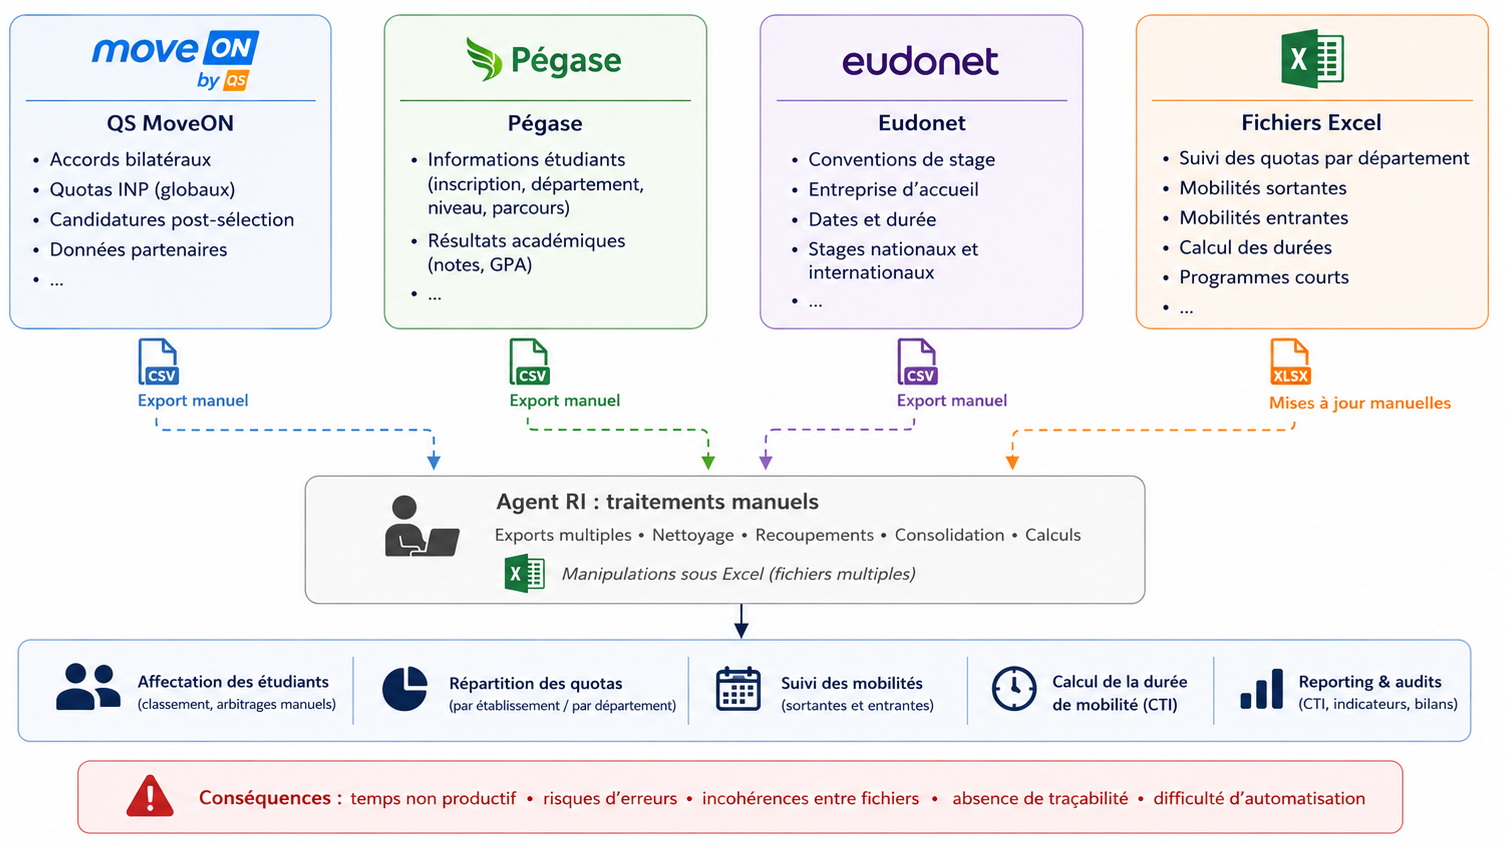
\includegraphics[width=0.90\textwidth]{figures/systemes/systeme-existant.png}
\caption{Système d'information existant du service RI}
\label{fig:systeme_existant}
\end{figure}

Cette absence de communication entre les outils crée plusieurs problèmes qui reviennent à chaque campagne.

\begin{itemize}
    \item \textbf{Des exports manuels à chaque étape.} Comme les outils ne communiquent pas entre eux, chaque consolidation de données nécessite des exports depuis plusieurs plateformes, puis une mise en forme dans Excel. Ce travail est long et source d'erreurs.

    \item \textbf{Une sélection sans règles fixes.} Les candidats sont classés manuellement à partir d'un tableau de GPA. En cas d'égalité ou de cas particulier, c'est l'agent RI qui tranche, et sa décision peut changer d'une année à l'autre sans qu'il y ait de trace écrite.

    \item \textbf{Des quotas insuffisamment détaillés.} MoveON ne gère les places qu'à l'échelle de l'INP global, sans distinguer les établissements qui le composent. La répartition par établissement (dont l'ENSEEIHT), puis par département pédagogique, est faite manuellement dans Excel, sans vérification de cohérence.

    \item \textbf{Des mobilités complémentaires non suivies.} Les summer schools, séjours linguistiques et programmes courts n'ont pas de place dans les outils existants. Pour les inclure dans le calcul de la durée de mobilité, l'agent doit s'en souvenir lui-même — ce qui n'est pas fiable.

    \item \textbf{Un calcul de durée de mobilité entièrement manuel et coûteux en temps.} Pour calculer la durée de mobilité d'un étudiant, il faut rassembler des données réparties dans trois systèmes différents (MoveON, Pégase, Eudonet) et les recouper à la main dans Excel. Selon les échanges avec le service RI, cette consolidation représente de l'ordre d'une dizaine de minutes par dossier, soit plusieurs journées de traitement cumulées à l'échelle d'une promotion de 300 étudiants — sans compter le risque d'oubli d'une période de mobilité à chaque manipulation. Cette opération ne peut pas être automatisée tant qu'il n'existe pas de source de données unifiée.
\end{itemize}

% ─────────────────────────────────────────────────────────────
\section{Problématique et solution envisagée}
% ─────────────────────────────────────────────────────────────

Cette section formule la problématique centrale du projet à partir du constat précédent, puis présente la solution envisagée dans ses grandes lignes. 

\subsection{Problématique}

Le service RI utilise plusieurs outils qui ne communiquent pas entre eux. Chaque transfert de données se fait à la main, l'affectation des étudiants n'a pas de règle fixe, et il n'existe pas de moyen simple de calculer la durée de mobilité. Cinq problèmes restent sans solution :

\begin{itemize}
  \item Les données sont dispersées entre plusieurs systèmes et ne peuvent pas être consultées depuis un seul endroit.
  \item Les quotas ne descendent pas jusqu'au niveau département, alors que c'est ce niveau qui détermine qui peut partir et où.
  \item La sélection des candidats se fait à la main, sans règle définie à l'avance.
  \item Le calcul de la durée de mobilité oblige à rassembler des données venant de plusieurs sources différentes.
  \item Les étudiants n'ont pas d'aide pour choisir leurs destinations.
\end{itemize}

C'est à partir de ce constat que se formule la question centrale du projet :

\begin{quote}
\textit{Comment concevoir une plateforme intégrée qui automatise le processus de gestion des mobilités internationales à l'ENSEEIHT, depuis la centralisation des données multi-sources jusqu'à l'affectation algorithmique, tout en garantissant la conformité CTI et l'aide à la décision des étudiants ?}
\end{quote}

\subsection{Solution envisagée}

La réponse envisagée est le développement d'une plateforme propre au service RI. Elle ne remplace pas les outils existants, mais se connecte à eux pour récupérer les données automatiquement. Elle doit permettre de gérer les quotas par département, de classer et affecter les étudiants selon des règles définies à l'avance, de calculer la durée de mobilité de façon automatique, et d'aider les étudiants à choisir leurs destinations. L'objectif est de centraliser les données et de réduire le travail manuel.

% ─────────────────────────────────────────────────────────────
\section{Besoins du système}
\label{sec:besoins-systeme}
% ─────────────────────────────────────────────────────────────

Cette section décrit les principales fonctionnalités attendues du système, les exigences non fonctionnelles associées, ainsi que les profils utilisateurs et le périmètre de réalisation retenu pour ce projet.

\subsection{Besoins fonctionnels}

Les besoins fonctionnels décrivent les principales fonctionnalités attendues du système afin de répondre aux problématiques identifiées au sein du service RI. Ils couvrent à la fois les fonctionnalités opérationnelles et les fonctionnalités intelligentes.

\subsubsection{Fonctionnalités opérationnelles}

Le système prend en charge les opérations suivantes, qui couvrent l'ensemble du cycle de gestion des mobilités internationales, de l'import des données jusqu'à l'archivage des résultats.

\begin{itemize}
    \item \textbf{BF01 --- Intégration des données} : import depuis MoveON, Pégase et Eudonet via API REST, et depuis des fichiers Excel pour les sources sans API. Chaque import inclut une détection de doublons, une validation des formats et un mécanisme de fallback Excel en cas d'indisponibilité d'une API.
    \item \textbf{BF02 --- Gestion des accords et quotas} : import des accords depuis MoveON et gestion de la répartition locale des places par département N7, avec possibilité d'ajustement manuel par le service RI.
    \item \textbf{BF03 --- Algorithme d'affectation} : pré-affectation automatique basée sur le GPA, les vœux ordonnés et les quotas par département, avec interface de supervision et d'ajustement.
    \item \textbf{BF04 --- Suivi de la durée de mobilité} : calcul automatique de la durée totale de mobilité de chaque étudiant, par agrégation des séjours académiques, stages et expériences complémentaires validées.
    \item \textbf{BF05 --- Mobilités complémentaires} : les étudiants déclarent leurs expériences et déposent les justificatifs nécessaires, puis le service RI se charge de la validation des dossiers.
    \item \textbf{BF06 --- Mobilités entrantes} : import via template Excel et suivi administratif granulaire.
    \item \textbf{BF07 --- Historisation} : les données d'une campagne clôturée passent en lecture seule. Aucune exécution ultérieure ne peut modifier les résultats d'une année passée.
    \item \textbf{BF08 --- Reporting et enquêtes CTI} : calcul automatique des indicateurs requis pour les enquêtes annuelles de la Commission des Titres d'Ingénieur — nombre et pourcentage d'étudiants mobiles, durée moyenne de mobilité, répartition des destinations — ainsi qu'export des rapports de conformité correspondants.
\end{itemize}

\subsubsection{Fonctionnalités intelligentes}

En complément des fonctionnalités opérationnelles, le système intègre deux modules intelligents qui améliorent l'expérience étudiant sans solliciter le service RI.

\begin{itemize}
    \item \textbf{BF09 --- Moteur de recommandation} : suggestions de destinations basées sur le GPA, le département et l'historique des affectations, pour orienter les choix de l'étudiant avant la saisie dans MoveON.
    \item \textbf{BF10 --- Assistant virtuel (chatbot RAG)} : agent conversationnel répondant aux questions procédurales à partir de la documentation institutionnelle, sans solliciter le service RI.
\end{itemize}

\subsection{Besoins non fonctionnels}

Au-delà des fonctionnalités métier, le système doit également répondre à plusieurs exigences techniques et organisationnelles. Ces besoins non fonctionnels concernent notamment la sécurité, la performance, l'intégrité des données et l'intégration avec l'environnement existant.

\begin{itemize}
    \item \textbf{BNF01 --- Interopérabilité} : le système doit s'intégrer sans rupture dans l'écosystème existant via des adaptateurs REST dédiés à chaque source. En cas d'indisponibilité d'une API, un fallback par import Excel garantit la continuité opérationnelle.

    \item \textbf{BNF02 --- Intégrité des données} : les données provenant de sources hétérogènes peuvent être incohérentes ou dupliquées. Une validation stricte est appliquée à chaque import — contrôle de format, détection de doublons, cohérence inter-sources. Toute donnée rejetée est tracée dans un rapport d'import avec la raison précise, pour correction ciblée.

    \item \textbf{BNF03 --- Sécurité et RGPD} : authentification via le SSO institutionnel, gestion stricte des rôles (étudiant vs administrateur), chiffrement des données sensibles. Un étudiant n'accède qu'à son propre dossier.

    \item \textbf{BNF04 --- Performance} : le temps de réponse de l'API pour les endpoints courants doit être inférieur à 200~ms sous une charge de 50 utilisateurs simultanés. L'algorithme d'affectation doit s'exécuter en moins de 30 secondes pour une promotion de 300 étudiants. Les traitements lourds — algorithme d'affectation, calculs CTI — sont exécutés de façon asynchrone en arrière-plan pour ne pas bloquer l'interface.

    \item \textbf{BNF05 --- Disponibilité} : s'agissant d'un système institutionnel sollicité lors de périodes de campagne critiques (ouverture des vœux, publication des résultats), une disponibilité cible de 99~\% hors fenêtres de maintenance planifiées est visée, appuyée par une politique de sauvegarde permettant une reprise rapide en cas d'incident.

    \item \textbf{BNF06 --- Scalabilité} : séparation entre données actives et données archivées en lecture seule pour absorber la croissance annuelle du volume historique et les pics de connexion lors des moments clés de campagne.

    \item \textbf{BNF07 --- Ergonomie} : l'interface adapte sa navigation et ses fonctionnalités au rôle de l'utilisateur connecté, réduisant les erreurs de manipulation.

    \item \textbf{BNF08 --- Traçabilité} : toute action importante — import, modification d'affectation, validation, transition de phase — est enregistrée avec l'identité de l'auteur et l'horodatage dans un journal d'audit persistant en écriture seule.
\end{itemize}

\subsection{Profils utilisateurs et périmètre de réalisation}

Cette sous-section présente les profils d'utilisateurs du système, puis définit le périmètre de réalisation retenu pour ce projet.

\subsubsection{Profils utilisateurs}

Deux profils utilisent le système, avec des besoins très différents.

\textbf{L'administrateur} — c'est-à-dire le service RI — pilote la campagne de bout en bout. Il supervise les imports, configure les quotas, ajuste les propositions d'affectation, instruit les demandes de mobilités complémentaires et produit les rapports CTI. Le système prend en charge les tâches répétitives, mais toute décision finale reste sous sa responsabilité, et chaque intervention manuelle est tracée.

\textbf{L'étudiant} consulte les destinations disponibles, reçoit des recommandations personnalisées avant de saisir ses vœux dans MoveON, suit l'état de sa candidature, déclare ses expériences complémentaires et vérifie à tout moment si sa durée totale de mobilité atteint le seuil requis pour l'obtention du diplôme. L'assistant virtuel répond à ses questions procédurales sans solliciter le service RI.

\subsubsection{Périmètre de réalisation}

Le développement est organisé en deux niveaux de priorité.

\textbf{MVP — fonctionnalités prioritaires (BF01 à BF08, BNF01 à BNF08)} :
\begin{itemize}
  \item Intégration des données multi-sources (MoveON, Pégase, Eudonet, Excel)
  \item Gestion des accords et quotas par département
  \item Algorithme d'affectation avec validation humaine
  \item Calcul automatique de la durée de mobilité
  \item Gestion des mobilités complémentaires et entrantes
  \item Reporting et enquêtes CTI : indicateurs chiffrés, tableaux de bord analytiques et exports de conformité
  \item Espace étudiant : catalogue, suivi de candidature, déclarations
  \item Sécurité : SSO, contrôle d'accès, audit log
\end{itemize}

\textbf{V2 — fonctionnalités secondaires (BF09, BF10)} :
\begin{itemize}
  \item Moteur de recommandation de destinations personnalisé
  \item Assistant virtuel (chatbot RAG)
\end{itemize}

% ─────────────────────────────────────────────────────────────
\section{Organisation et cadrage du projet}
% ─────────────────────────────────────────────────────────────

Cette section regroupe les éléments qui cadrent la conduite du projet : la méthodologie de gestion de projet retenue, la planification générale et l'environnement de travail utilisé.

\subsection{Méthodologie de gestion de projet}

Le projet s'étend sur six mois dans un contexte où certaines règles métier
n'étaient pas complètement formalisées dès le départ. Trois approches ont été
évaluées avant de retenir la méthodologie la mieux adaptée.

\subsubsection{Méthode en cascade}

La méthode en cascade organise le projet en phases séquentielles et strictement
ordonnées : analyse, conception, développement, test, déploiement. Chaque phase
doit être complètement terminée avant de passer à la suivante.

\textbf{Avantages :} Elle offre une planification claire et une documentation
exhaustive dès le départ, ce qui facilite le suivi et la traçabilité des décisions.

\textbf{Limites dans notre contexte :} Elle impose de geler un cahier des charges
complet avant tout développement. Or, certaines règles métier — notamment la
hiérarchie des quotas et les critères de priorité dans l'affectation — n'étaient
pas entièrement définies au démarrage du projet, rendant cette approche inadaptée.

\subsubsection{Kanban}

Kanban est une méthode de gestion de flux continu, sans itérations fixes. Le
travail est visualisé sur un tableau et les tâches avancent au fur et à mesure
de la disponibilité de l'équipe.

\textbf{Avantages :} Sa flexibilité permet de s'adapter rapidement aux changements
et de traiter les tâches par ordre de priorité sans contrainte de cycle.

\textbf{Limites dans notre contexte :} L'absence d'itérations fixes et de
jalons structurés le rend peu adapté à un projet avec un périmètre défini et
une date de livraison fixe, où une planification rigoureuse est nécessaire.

\subsubsection{Scrum}

Scrum est un cadre agile qui organise le développement en sprints de durée fixe,
avec des événements régulières (planning, review, retrospective) et un backlog
priorisé.

\textbf{Avantages :} Il offre un bon équilibre entre structure et flexibilité :
les priorités peuvent être révisées à chaque sprint, les livraisons sont
incrémentales et validables régulièrement par le service RI.

\textbf{Limites dans notre contexte :} Scrum est conçu pour des équipes. Certains
événements, comme le Daily Scrum ou la rétrospective d'équipe, supposent une
coordination quotidienne entre plusieurs personnes et ne s'appliquent pas tels
quels à un projet porté par une seule développeuse ; ils doivent être adaptés
ou remplacés par des pratiques équivalentes.

\subsubsection{Comparaison et choix retenu}

Le tableau~\ref{tab:methodo_comparaison} compare les trois approches sur des critères objectifs.

\renewcommand{\arraystretch}{1.4}
\begin{table}[H]
\centering
\footnotesize
\begin{tabular}{|p{3cm}|p{3cm}|p{3cm}|p{3cm}|}
\hline
\rowcolor{gray!20}
\textbf{Critère} & \textbf{Cascade} & \textbf{Kanban} & \textbf{Scrum} \\
\hline
Planification & Rigide dès le début & Continue, sans itérations fixes & Sprints fixes avec rétroplanification \\
\hline
Adaptation aux changements & Difficile & Bonne, mais sans rythme structuré & Bonne, intégrée à chaque sprint \\
\hline
Visibilité client & Faible en cours de projet & Modérée & Élevée (Sprint Review) \\
\hline
\end{tabular}
\caption{Comparaison des approches de gestion de projet}
\label{tab:methodo_comparaison}
\end{table}

Au regard de ces trois critères, Scrum est le seul à combiner une planification structurée et une capacité d'adaptation intégrée à chaque itération, tout en offrant la meilleure visibilité pour le service RI. C'est pourquoi \textbf{Scrum} est retenu, pour son équilibre entre structure (sprints de durée
fixe, backlog priorisé) et flexibilité (révision des priorités à chaque sprint,
livraisons incrémentales validables par le service RI). Ce cadre étant conçu
pour une équipe, son application est toutefois adaptée au contexte d'un
développement individuel : certains rôles et événements sont ajustés ou
remplacés par des pratiques équivalentes, comme précisé ci-dessous.

Scrum s'appuie sur des rôles, des artefacts et des événements, présentés
ci-dessous et adaptés au contexte d'un stage individuel.

\subsubsection{Les rôles Scrum}

\begin{itemize}[label=•]
    \item \textit{\textbf{Le Product Owner}} : responsable de la priorisation du backlog et de la validation des livraisons.
    \item \textit{\textbf{Le Scrum Master}} : chargé du suivi de l'avancement, de la levée des blocages et de l'orientation technique.
    \item \textit{\textbf{L'équipe de développement (Development Team)}} : réalise les incréments du produit. Ce rôle est habituellement porté par plusieurs personnes ; dans ce projet, il est assuré par une seule personne, responsable de l'intégralité du développement.
\end{itemize}

Le tableau~\ref{tab:roles-scrum} précise, pour ce projet, la personne assurant chacun de ces rôles.

\renewcommand{\arraystretch}{1.5}
\begin{table}[H]
\centering
\begin{tabular}{|p{5cm}|p{7cm}|}
\hline
\rowcolor{gray!20}
\textbf{Rôle Scrum} & \textbf{Personne(s)} \\
\hline
Product Owner & Service RI  \\
\hline
Scrum Master & Madame Myriam FOURATI  \\
\hline
Development Team & Ons SOUISSI \\
\hline
\end{tabular}
\caption{Rôles Scrum et responsables associés}
\label{tab:roles-scrum}
\end{table}

\subsubsection{Les artefacts Scrum}

\begin{itemize}[label=•]
    \item \textit{\textbf{Le backlog du produit}} : liste des fonctionnalités du système, priorisées selon la méthode MoSCoW et estimées en story points ; détaillé au chapitre~4 (Product Backlog).
    \item \textit{\textbf{Le backlog de sprint}} : sous-ensemble du backlog produit retenu pour un sprint donné ; présenté pour chaque sprint réalisé au chapitre~5.
    \item \textit{\textbf{L'incrément}} : ensemble des fonctionnalités terminées à l'issue d'un sprint, qui s'ajoute aux incréments précédents.
\end{itemize}

\subsubsection{Les événements Scrum}

\begin{itemize}[label=•]
    \item \textit{\textbf{Le Sprint}} : période de développement à durée fixe (deux à trois semaines dans ce projet), à l'issue de laquelle un incrément fonctionnel est livré.
    \item \textit{\textbf{Sprint Planning}} : réunion de début de sprint au cours de laquelle les user stories du sprint sont sélectionnées et décomposées en tâches.
    \item \textit{\textbf{Sprint Review}} : réunion de fin de sprint au cours de laquelle les fonctionnalités livrées sont démontrées au service RI (Product Owner), qui valide ou ajuste les priorités du backlog.
    \item \textit{\textbf{Daily Scrum}} : dans sa forme standard, synchronisation quotidienne entre les membres de l'équipe de développement. Cet événement suppose une coordination entre plusieurs personnes et n'a donc pas de sens pour un projet porté par une seule développeuse ; il n'est pas mis en œuvre.
    \item \textit{\textbf{Sprint Retrospective}} : dans sa forme standard, réunion d'équipe de fin de sprint destinée à identifier les points à améliorer. Dans le cadre de ce projet individuel, elle est remplacée par un bilan personnel de fin de sprint, réalisé sans réunion dédiée, permettant de vérifier les tâches restantes et d'ajuster en conséquence le contenu du sprint suivant.
\end{itemize}

Le suivi du backlog est géré avec GitHub Projects, chaque user story
correspondant à une issue liée aux pull requests qui l'implémentent.

\subsection{Planification générale}

Le projet s'est déroulé sur six mois, organisés en cinq grandes phases dont l'enchaînement est résumé dans le tableau~\ref{tab:planning-general}. La planification détaillée sprint par sprint, sous forme de product backlog et de diagramme de Gantt, ne pouvait être établie qu'une fois le périmètre fonctionnel et les choix technologiques stabilisés ; elle est donc présentée au chapitre~4 (Conception du système).

\renewcommand{\arraystretch}{1.4}
\begin{table}[H]
\centering
\footnotesize
\begin{tabular}{|p{1cm}|p{7.5cm}|p{4.5cm}|}
\hline
\rowcolor{gray!20}
\textbf{Phase} & \textbf{Contenu} & \textbf{Durée indicative} \\
\hline
1 & Cadrage, analyse de l'existant et positionnement par rapport aux solutions existantes (chapitres 1 et 2) & 3 à 4 semaines \\
\hline
2 & Choix technologiques et algorithmiques (chapitre 3) & 2 semaines \\
\hline
3 & Conception détaillée : product backlog, architecture, modèle de données (chapitre 4) & 2 à 3 semaines \\
\hline
4 & Réalisation itérative en sprints Scrum (chapitre 5) & environ 3 mois \\
\hline
5 & Tests de charge et de sécurité, documentation, livraison & 2 à 3 semaines \\
\hline
\end{tabular}
\caption{Planification générale du projet}
\label{tab:planning-general}
\end{table}

\section*{Conclusion}
\justifying
\phantomsection
\addcontentsline{toc}{section}{Conclusion}

Ce chapitre a présenté l'organisme d'accueil, analysé les limites du système d'information existant, formulé la problématique et la solution envisagée, précisé les besoins du système et posé le cadrage du projet. Il reste toutefois à vérifier qu'aucune solution du marché ne répond déjà à ce besoin : c'est l'objet du chapitre suivant, qui positionne ce projet par rapport aux solutions existantes.

   \clearpage

% !TEX root = ../main.tex
% ══════════════════════════════════════════════════════════════
\chapter{Positionnement par rapport aux solutions existantes}
% ══════════════════════════════════════════════════════════════
\begingroup
\let\clearpage\relax
\startcontents[chapters]
\printcontents[chapters]{}{1}{\section*{Plan}}
\endgroup
\newpage

\section*{Introduction}
\justifying
\phantomsection
\addcontentsline{toc}{section}{Introduction}

Le chapitre précédent a mis en évidence les limites du système d'information du service RI et formulé la problématique du projet. Ce chapitre évalue les solutions existantes au regard des huit critères qui en découlent, afin de vérifier qu'aucune ne répond déjà à ces besoins avant d'engager le développement d'une solution sur mesure.

% ─────────────────────────────────────────────────────────────
\section{Grille d'évaluation}
% ─────────────────────────────────────────────────────────────

Pour comparer les solutions de façon rigoureuse, une grille de huit critères a été définie
à partir des problèmes concrets identifiés au chapitre précédent. Chaque critère traduit une
lacune précise du système actuel. Le tableau~\ref{tab:grille_eval} présente cette grille.

\renewcommand{\arraystretch}{1.45}
\begin{table}[H]
\centering
\footnotesize
\begin{tabular}{|p{0.6cm}|p{3.8cm}|p{9.2cm}|}
\hline
\rowcolor{gray!20}
\textbf{\#} & \textbf{Critère} & \textbf{Ce que cela signifie concrètement pour l'ENSEEIHT} \\
\hline
C1 & Centralisation des données de mobilité & Regrouper dans une seule plateforme
l'ensemble des données relatives aux mobilités sortantes, entrantes, complémentaires
et aux stages internationaux, ainsi que les données académiques des étudiants \\
\hline
C2 & Quotas par école et par département & Gestion des places allouées d'abord à l'échelle de l'ENSEEIHT, puis par département pédagogique (SN, 3EA, MF2E), et non uniquement à l'échelle globale INP \\
\hline
C3 & Aide à la décision et auto-affectation & Présence d'un mécanisme automatique de classement et de pré-affectation des candidats. \\
\hline
C4 & Calcul de la durée de mobilité & Agrégation automatique de toutes les périodes de mobilité d'un étudiant (académique, stage, complémentaire) pour produire la durée réglementaire \\
\hline
C5 & Mobilités complémentaires & Prise en charge des expériences hors accord bilatéral (summer schools, séjours linguistiques, programmes courts) avec dépôt et validation de justificatifs \\
\hline
C6 & Adaptabilité aux règles internes & Capacité du système à fonctionner selon les règles propres à l'établissement : priorités d'affectation, seuils de sélection, critères locaux \\
\hline
C7 & Recommandation de destinations & Suggestion de destinations adaptées au profil de l'étudiant (département, GPA, langue, préférences) pour l'accompagner dans son choix \\
\hline
C8 & Reporting CTI & Production automatique des indicateurs clés (KPIs) exigés par la CTI, notamment : taux de mobilité par promotion, durée moyenne de mobilité par étudiant, et répartition géographique des destinations \\
\hline
\end{tabular}
\caption{Grille d'évaluation des solutions existantes}
\label{tab:grille_eval}
\end{table}

% ─────────────────────────────────────────────────────────────
\section{Analyse des solutions existantes}
% ─────────────────────────────────────────────────────────────

Quatre solutions ont été examinées : QS MoveON, déjà utilisé par le service RI, Mobility-Online, une plateforme européenne largement déployée dans les services de relations internationales, ErasmusJET, développé dans le cadre du programme Erasmus+, et les travaux académiques d'Elahi et al. sur la recommandation de destinations.

\subsection{QS MoveON}

MoveON est l'outil central du service RI pour la gestion des accords bilatéraux et des candidatures. Il est examiné ici non pas pour le remplacer, mais pour identifier précisément ce qu'il ne couvre pas~\cite{qs_moveon}.

\textbf{Points forts  :} le référentiel des accords bilatéraux, le suivi des candidatures post-sélection et l'administration des dossiers étudiants. Son API REST est un point d'appui utile pour extraire les données.

\textbf{Limites par rapport aux critères définis :}

\begin{itemize}
    \item MoveON se limite aux mobilités sortantes et aux accords. Les données académiques (GPA, département, parcours), les stages internationaux et les mobilités complémentaires en sont totalement absents. Le service RI est donc contraint d'exporter depuis MoveON, de compléter à la main dans Excel, puis de travailler sur ce fichier hybride — ce cumul de gestes est exactement ce que ce projet cherche à éliminer.

    \item Les quotas ne sont gérés qu'à l'échelle INP. La déclinaison par école (ENSEEIHT) puis par département pédagogique, qui conditionne l'affectation interne, est entièrement tenue dans des fichiers Excel sans aucune contrainte de cohérence.

    \item Aucun classement automatique n'existe. La sélection est intégralement manuelle, ce qui signifie que les règles appliquées varient selon l'agent et la campagne.

    \item Sans les stages ni les expériences complémentaires, le calcul de la durée de mobilité est impossible à automatiser depuis MoveON seul.

    \item Aucune suggestion de destinations adaptée au profil de l'étudiant.

    \item Les exports MoveON ne produisent pas les indicateurs CTI structurés (taux de mobilité par promotion, durées moyennes, répartition géographique) dans un format directement exploitable pour les audits.
\end{itemize}

MoveON reste un bon outil pour ce qu'il fait, mais sa conception ne prévoit pas de
couvrir les besoins opérationnels internes d'un établissement.

\subsection{Mobility-Online}

Mobility-Online est une plateforme de gestion de la mobilité étudiante largement utilisée par des services de relations internationales en Europe, notamment pour la gestion administrative des échanges Erasmus+ et des accords bilatéraux.

\textbf{Points forts :} un module de gestion documentaire complet (conventions, learning agreements, relevés de notes) et une bonne couverture du suivi administratif des mobilités entrantes et sortantes, sur un périmètre européen large.

\textbf{Limites par rapport aux critères définis :}

\begin{itemize}
    \item La plateforme est conçue comme un outil de gestion administrative générique, sans granularité de quotas par département pédagogique propre à un établissement français comme l'ENSEEIHT.
    \item Aucun mécanisme d'auto-affectation basé sur le classement académique n'est proposé : la sélection reste manuelle.
    \item Le calcul de durée de mobilité selon les critères CTI, spécifiques aux écoles d'ingénieurs françaises, n'est pas pris en charge, la plateforme n'étant pas conçue pour ce cadre réglementaire.
    \item Ni recommandation de destinations personnalisée, ni reporting structuré selon les indicateurs CTI.
\end{itemize}

Mobility-Online confirme qu'une plateforme généraliste, même mature et largement déployée, ne couvre pas les besoins spécifiques d'un établissement soumis aux exigences de la CTI.

\subsection{ErasmusJET}

ErasmusJET est une plateforme développée dans le cadre des initiatives de digitalisation du programme Erasmus+. Son objectif est de standardiser les échanges de données entre établissements partenaires du réseau européen.

\textbf{Points forts :} la gestion complète du cycle Erasmus — dépôt de candidatures en ligne, génération et signature des conventions, échange de relevés de notes entre institutions. Pour un établissement dont toutes les mobilités relèvent du programme Erasmus, c'est une solution adaptée.

\textbf{Limites par rapport aux critères définis :}

\begin{itemize}
    \item ErasmusJET ne fonctionne que pour Erasmus+. Les accords hors Europe — qui représentent une grande partie des mobilités de l'ENSEEIHT — restent en dehors de son périmètre, tout comme les données académiques, les stages et les mobilités complémentaires.

    \item Les quotas par département, l'auto-affectation et le calcul de durée CTI ne sont pas prévus dans la plateforme.

    \item Son format est standardisé pour les échanges européens, ce qui ne laisse pas de place pour les règles propres à chaque établissement.

    \item Ni recommandation de destinations, ni reporting CTI.
\end{itemize}

ErasmusJET peut être utile pour la partie Erasmus+, mais il ne règle aucun des problèmes identifiés.

\subsection{Travaux académiques : Elahi et al. (2022)}

Les travaux d'Elahi et al. proposent un système qui combine recommandation de destinations et processus d'affectation étudiante. Les tests sont réalisés sur un jeu de données simulé~\cite{Elahi2022}.

\textbf{Points forts :} c'est la seule des solutions analysées qui aborde sérieusement le critère C7 — la recommandation personnalisée de destinations. L'article démontre la faisabilité technique de coupler un algorithme de suggestion avec un processus de sélection, ce qui en fait une référence directement pertinente pour la partie intelligence du projet.

\textbf{Limites par rapport aux critères définis :}

\begin{itemize}
    \item Le modèle repose sur un dataset simulé et uniforme, sans connexion avec des systèmes institutionnels réels. Il ne propose aucune intégration avec MoveON, Pégase ou Eudonet.

    \item La gestion des quotas par département, l'affectation sous contraintes, le calcul de durée de mobilité et les expériences complémentaires sont entièrement hors du périmètre — le modèle ne traite que la recommandation.

    \item C'est un prototype de recherche : il n'y a aucun moyen de configurer des règles propres à un établissement.

    \item Le reporting CTI n'est pas abordé.
\end{itemize}

Ces travaux sont une référence utile pour la partie recommandation, mais ils ne forment pas une solution prête à être utilisée à l'ENSEEIHT.

% ─────────────────────────────────────────────────────────────
\section{Tableau comparatif de synthèse}
% ─────────────────────────────────────────────────────────────

Le tableau~\ref{tab:synthese_solutions} résume la couverture de chaque solution pour les huit critères de la grille d'évaluation. La légende suivante s'applique : \cmark\ = critère satisfait, \xmark\ = critère non satisfait, \textit{Partiel} = critère partiellement couvert.

\renewcommand{\arraystretch}{1.45}
\begin{table}[H]
\centering
\footnotesize
\begin{tabular}{|p{5.4cm}|>{\centering\arraybackslash}p{2cm}|>{\centering\arraybackslash}p{2.1cm}|>{\centering\arraybackslash}p{2cm}|>{\centering\arraybackslash}p{2.1cm}|}
\hline
\rowcolor{gray!20}
\centering{\textbf{Critère}} & \textbf{QS MoveON} & \textbf{Mobility-Online} & \textbf{ErasmusJET} & \textbf{Elahi et al.} \\
\hline
C1 – Centralisation des données & Partiel & Partiel & \xmark & \xmark \\
\hline
C2 – Quotas par école et département & \xmark & \xmark & \xmark & \xmark \\
\hline
C3 – Aide à la décision et auto-affectation & \xmark & \xmark & \xmark & \xmark \\
\hline
C4 – Calcul durée de mobilité & \xmark & \xmark & \xmark & \xmark \\
\hline
C5 – Mobilités complémentaires & \xmark & \xmark & \xmark & \xmark \\
\hline
C6 – Adaptabilité métier & Partiel & \xmark & \xmark & \xmark \\
\hline
C7 – Recommandation de destinations & \xmark & \xmark & \xmark & Partiel \\
\hline
C8 – Reporting CTI & \xmark & \xmark & \xmark & \xmark \\
\hline
\end{tabular}
\caption{Synthèse comparative des solutions selon la grille d'évaluation}
\label{tab:synthese_solutions}
\end{table}

Aucune des quatre solutions étudiées — qu'il s'agisse d'outils commerciaux largement déployés (MoveON, Mobility-Online), d'une initiative institutionnelle européenne (ErasmusJET) ou d'un prototype de recherche (Elahi et al.) — ne répond à l'ensemble des besoins identifiés. Ce résultat, obtenu sur un panel volontairement diversifié, confirme la nécessité de développer une solution propre au service RI, conformément à la problématique et à la solution envisagées au chapitre précédent.

\section*{Conclusion}
\justifying
\phantomsection
\addcontentsline{toc}{section}{Conclusion}

Ce chapitre a montré qu'aucune des solutions existantes — commerciales ou académiques — ne couvre les huit critères identifiés, en particulier la granularité des quotas par département et la conformité CTI, propres au contexte français. Ce constat valide la solution envisagée au chapitre précédent ; le chapitre suivant en détaille les choix technologiques et algorithmiques.

    \clearpage

% !TEX root = ../main.tex
% ══════════════════════════════════════════════════════════════
\chapter{Choix technologiques et algorithmiques}
\label{cha:choix-technologiques}
% ══════════════════════════════════════════════════════════════
\begingroup
\let\clearpage\relax
\startcontents[chapters]
\printcontents[chapters]{}{1}{\section*{Plan}}
\endgroup
\newpage

\section*{Introduction}
\justifying
\phantomsection
\addcontentsline{toc}{section}{Introduction}

Le chapitre précédent a montré qu'aucune solution existante ne répondait aux besoins du service RI, d'où le choix de développer une plateforme sur mesure. Ce chapitre justifie les technologies et les algorithmes retenus pour la construire, en comparant à chaque fois les principales alternatives.

% ─────────────────────────────────────────────────────────────
\section{Choix du frontend}
% ─────────────────────────────────────────────────────────────

Cette section présente les besoins spécifiques du frontend, évalue les
alternatives disponibles, puis justifie le choix retenu.

\subsection{Besoins spécifiques}

L'interface du projet doit couvrir deux espaces bien
distincts : d'un côté, un espace dédié au service RI
pour piloter les campagnes, de l'autre, un espace
étudiant pour consulter les destinations, suivre
sa candidature et interagir avec le chatbot.
Certaines pages affichent des données sensibles
(résultats d'affectation, GPA) et doivent être
construites côté serveur pour éviter qu'elles
ne soient accessibles avant que le rôle de
l'utilisateur soit vérifié. D'autres, comme
le suivi de candidature ou le chatbot,
nécessitent une navigation fluide et réactive.
Gérer ces deux types de pages dans le même projet,
avec une séparation fiable des accès selon le rôle,
est le principal critère de choix.

\subsection{Alternatives évaluées}

Trois frameworks ont été évalués au regard des besoins identifiés.

\subsubsection{Applications monopage — React + Vite}

React  permet de construire des interfaces
entièrement rendues dans le navigateur ~\cite{react_dev}.

\textit{Avantages :}
\begin{itemize}
  \item Simple à configurer et à démarrer
  \item Très bien documenté, avec de nombreuses
        ressources disponibles en ligne
\end{itemize}

\textit{Limites :}
\begin{itemize}
  \item Tout est chargé et affiché dans le navigateur :
        les données sensibles comme les affectations
        ou les GPA y arrivent avant même que
        le rôle de l'utilisateur soit contrôlé,
        ce qui fragilise la séparation entre
        l'espace étudiant et l'espace RI
  \item La protection des pages selon le rôle
        doit être codée manuellement, sans
        mécanisme intégré pour l'imposer
        au niveau du routing
  \item Les appels à l'API Django passent tous
        par le navigateur, ce qui expose
        les tokens d'authentification au client
\end{itemize}

\subsubsection{Angular}

Angular est un framework TypeScript développé
par Google, utilisé principalement pour des
applications d'entreprise avec beaucoup de
logique interne ~\cite{angular_dev}.

\textit{Avantages :}
\begin{itemize}
  \item Architecture très structurée, adaptée aux
        applications avec de nombreux écrans
        et règles métier
  \item Typage TypeScript natif, ce qui réduit
        les erreurs au moment du développement
  \item Mécanisme de protection des routes intégré,
        utile pour séparer les accès
        selon le rôle utilisateur
  \item Bien adapté à des interfaces
        d'administration complexes
        comme le tableau de bord RI
\end{itemize}

\textit{Limites :}
\begin{itemize}
  \item Pas de rendu côté serveur sans
        Angular Universal, qui nécessite
        une configuration supplémentaire
        non négligeable
  \item Angular demande un temps de prise en main
        important : son architecture impose
        de nombreux concepts spécifiques
        (modules, décorateurs, injection de
        dépendances) qui ralentissent
        le démarrage
  \item Moins d'exemples disponibles que
        React/Next.js pour l'intégration
        avec le SSO CAS utilisé
        par Toulouse INP
\end{itemize}

\subsubsection{Next.js 14}

Next.js est un framework basé sur React qui permet de combiner rendu côté serveur
et rendu côté client selon les besoins de chaque page ~\cite{nextjs_dev}.

\textit{Avantages :}
\begin{itemize}
  \item Rendu hybride : pages sensibles rendues côté serveur, composants
        interactifs côté client, les deux coexistant dans le même projet
  \item Middleware intégré pour bloquer l'accès aux pages selon le rôle
        utilisateur avant même leur chargement
  \item Appels à l'API Django réalisables côté serveur, sans exposer
        les tokens dans le navigateur
  \item App Router et React Server Components : chaque composant est rendu
        côté serveur par défaut, avec des layouts partagés par espace
        (RI, étudiant) qui structurent naturellement la séparation des interfaces
  \item TypeScript, Tailwind CSS et intégration SSO CAS/OIDC bien documentés
\end{itemize}

\textit{Limites :}
\begin{itemize}
  \item Configuration initiale un peu plus complexe qu'une application
        monopage classique
\end{itemize}

\subsection{Synthèse comparative}

Le tableau~\ref{tab:comparaison_frontend} récapitule les critères évalués pour chacune des trois solutions, afin de faciliter la comparaison et de justifier le choix retenu.

\renewcommand{\arraystretch}{1.35}
\begin{table}[H]
\centering
\caption{Comparaison des frameworks frontend}
\label{tab:comparaison_frontend}
\footnotesize
\begin{tabular}{|p{3.8cm}|>{\centering\arraybackslash}p{2.8cm}|>{\centering\arraybackslash}p{2.4cm}|>{\centering\arraybackslash}p{3cm}|}
\hline
\rowcolor{gray!20}
\textbf{Critère} & \textbf{React + Vite} & \textbf{Angular} & \textbf{Next.js 14} \\
\hline
Rendu côté serveur (SSR) & \xmark & Via Angular Universal (config requise) & \cmark \\
\hline
Protection des routes par rôle & Manuelle & Mécanisme intégré & Middleware intégré \\
\hline
Données sensibles côté serveur & \xmark & \xmark & \cmark \\
\hline
TypeScript natif & Optionnel & \cmark & \cmark \\
\hline
Intégration SSO CAS/OIDC & \cmark & Peu d'exemples avec le SSO CAS de Toulouse INP & \cmark \\
\hline
Rendu hybride SSR + CSR & \xmark & \xmark & \cmark \\
\hline
\end{tabular}
\end{table}

\subsection{Décision}

\textbf{Next.js 14} est retenu. Son modèle de React Server
Components permet de gérer naturellement les deux espaces du projet : les pages
sensibles du tableau de bord RI sont rendues côté serveur avant toute vérification
de rôle, tandis que les composants interactifs de l'espace étudiant s'exécutent côté client. Angular pourrait, en théorie, répondre au même besoin grâce à Angular Universal. Mais avec le temps disponible pour ce projet, Next.js permettait d'arriver au même résultat plus rapidement et avec moins de configuration à mettre en place.


% ─────────────────────────────────────────────────────────────
\section{Choix du backend}
% ─────────────────────────────────────────────────────────────

Cette section présente les besoins spécifiques du backend, évalue les
alternatives disponibles, puis justifie le choix retenu.

\subsection{Besoins spécifiques}

Le backend de ce projet ne se limite pas à une simple gestion de données. Il doit orchestrer de nombreuses entités métier liées entre elles et gérer des processus parfois complexes, comme le suivi des candidatures, des affectations ou des mobilités étudiantes.

L'application doit également assurer plusieurs fonctions essentielles : gérer les droits d'accès selon les profils (étudiants et administrateurs RI), conserver une trace des actions importantes via un journal d'audit, accompagner l'évolution de la base de données pendant le développement, et s'intégrer au système d'authentification institutionnel CAS/OIDC de Toulouse INP.

Dans ce contexte, le choix du framework ne repose pas uniquement sur les performances, mais aussi sur la qualité des outils qu'il apporte pour structurer, sécuriser et faire évoluer l'application.

\subsection{Choix du framework backend}

Cette sous-section évalue les frameworks backend candidats au regard des besoins définis ci-dessus, puis justifie le choix retenu.

\subsubsection{Alternatives évaluées}

Trois frameworks ont été évalués en regard des besoins identifiés précédemment.

\paragraph{Node.js}
Environnement d'exécution JavaScript côté serveur,
reconnu pour ses performances sur les applications
qui traitent beaucoup de requêtes simultanées ~\cite{nodejs_dev}.

\textit{Avantages :}
\begin{itemize}
  \item Bonnes performances sur les traitements
        non bloquants
  \item Grand nombre de bibliothèques disponibles
  \item Gestion native des opérations asynchrones
\end{itemize}

\textit{Limites :}
\begin{itemize}
    \item Aucun outil natif pour la base de données, l'administration ou la gestion des droits : il faut tout assembler manuellement à partir de bibliothèques séparées, ce qui alourdit la configuration et la maintenance.
    \item Des bibliothèques de machine à états comme XState existent et sont matures, mais rien d'équivalent à \texttt{django-fsm} n'est directement intégré à un ORM Node.js : il faudrait câbler soi-même la protection des transitions et la traçabilité fine des modifications au niveau des modèles, ce qui est indispensable dans ce projet.
    \item L'utilisation de Node.js implique de travailler en JavaScript, alors que le reste du système est conçu en Python, ce qui introduit une complexité supplémentaire en termes de cohérence et de maintenance.
    \item La gestion des évolutions du schéma de base de données au fil des sprints demande davantage d'efforts d'organisation et de suivi, car elle n'est pas aussi intégrée nativement dans l'écosystème.
\end{itemize}

\paragraph{FastAPI}
Framework Python récent, conçu pour construire
des APIs performantes avec une validation
automatique des données ~\cite{fastapi_dev}.

\textit{Avantages :}
\begin{itemize}
  \item Très bonnes performances grâce
        au support natif des requêtes asynchrones
  \item Validation automatique des données entrantes
  \item Documentation de l'API générée automatiquement
\end{itemize}

\textit{Limites :}
\begin{itemize}
  \item Pas d'outil intégré pour la base de données,
        l'administration ou la gestion des droits
  \item Les cycles de vie des entités,
        le journal d'audit et les permissions
        seraient à construire de zéro
  \item L'outil de migration de schéma demande davantage de configuration et d'intervention manuelle, ce qui peut ralentir les cycles d'itération en développement.
  \item FastAPI est surtout adapté à des APIs légères et rapides, et moins à des applications contenant beaucoup de logique métier.
\end{itemize}

\paragraph{Django}
Framework Python complet, pensé pour développer
rapidement des applications web avec beaucoup
de logique interne ~\cite{django_dev}.

\textit{Avantages :}
\begin{itemize}
  \item Gestion de la base de données,
        authentification, permissions et interface
        d'administration fournis nativement,
        sans aucune configuration supplémentaire
  \item \texttt{django-fsm} permet de définir
        des cycles de vie sécurisés sur chaque entité,
        avec une option qui empêche toute
        modification directe du statut
        en dehors des transitions autorisées
  \item \texttt{django-auditlog} enregistre
        automatiquement toutes les modifications
        avec l'auteur et la date, ce qui est indispensable
        pour les décisions réglementaires
  \item La gestion des évolutions de schéma
        est intégrée nativement, ce qui
        facilite les changements à chaque sprint
  \item S'intègre facilement avec le SSO CAS/OIDC
        via des bibliothèques existantes et maintenues
\end{itemize}

\textit{Limites :}
\begin{itemize}
  \item Django était historiquement limité
        sur les traitements asynchrones,
        mais cette lacune a été corrigée
        depuis la version 5
  \item Légèrement moins performant que FastAPI
        sur des calculs très complexes,
        ce qui peut être contourné en passant
        par des requêtes SQL directes
        pour les agrégations de durées CTI
\end{itemize}

\subsubsection{Synthèse comparative}

Le tableau~\ref{tab:comparaison_backend} récapitule les critères évalués pour chacune des trois solutions, afin de faciliter la comparaison et de justifier le choix retenu.

\renewcommand{\arraystretch}{1.35}
\begin{table}[H]
\centering
\caption{Comparaison des frameworks backend}
\label{tab:comparaison_backend}
\footnotesize
\begin{tabular}{|p{5cm}|>{\centering\arraybackslash}p{2.4cm}|>{\centering\arraybackslash}p{2.4cm}|>{\centering\arraybackslash}p{3.2cm}|}
\hline
\rowcolor{gray!20}
\textbf{Critère} & \textbf{Node.js} & \textbf{FastAPI} & \textbf{Django 5} \\
\hline
ORM et gestion BDD intégrés & \xmark & \xmark & \cmark \\
\hline
Interface d'administration & \xmark & \xmark & \cmark \\
\hline
Machines à états (FSM) & \xmark & \xmark & \cmark \\
\hline
Migrations de schéma & Manuel & nécessite config & \cmark \\
\hline
Authentification SSO & Manuel & Manuel & \cmark \\
\hline
Journal d'audit automatique & Manuel & Manuel & \cmark \\
\hline
Support ASGI / async & \cmark & \cmark & \cmark \\
\hline
\end{tabular}
\end{table}

\subsubsection{Décision}
\textbf{Django 5} est retenu car le projet repose sur de nombreuses entités liées entre elles, avec des cycles de vie distincts, un journal d'audit obligatoire et une gestion fine des droits entre deux profils utilisateurs.

Utiliser une autre solution aurait impliqué de reconstruire une grande partie de ces mécanismes.

Django permet de disposer de ces fonctionnalités directement, ce qui est un avantage important dans ce projet.

% Pour le déploiement en production, la configuration retenue est \textbf{Gunicorn} avec l'option \texttt{-k uvicorn.workers.UvicornWorker} : Gunicorn orchestre les workers et gère les signaux système, tandis que UvicornWorker assure le support natif de l'interface ASGI requise par Django Ninja pour les endpoints asynchrones.

% ─────────────────────────────────────────────────────────────
\subsection{Choix de la couche API}

Une fois le framework backend retenu, il reste à choisir la bibliothèque
la mieux adaptée pour construire l'API. Cette section évalue les deux
solutions compatibles avec Django et justifie le choix retenu.

\subsubsection{Besoins spécifiques}

L'API doit permettre les échanges entre Next.js
et Django, valider des structures de données
parfois complexes (vœux ordonnés, quotas par
département, rapports d'import), générer
automatiquement une documentation utilisable
par le développeur frontend, et répondre
de façon non bloquante aux requêtes qui
déclenchent des traitements longs
(lancement de l'algorithme, recalcul).

\subsubsection{Alternatives évaluées}

Deux solutions ont été évaluées pour exposer l'API entre le frontend Next.js et le backend Django.

\paragraph{Django REST Framework (DRF)}
Django REST Framework est la bibliothèque la plus utilisée pour construire
des APIs avec Django. Elle fournit un ensemble complet d'outils pour
la sérialisation, la validation et la gestion des permissions~\cite{drf_dev}.

\textit{Avantages :}
\begin{itemize}
  \item Très mature et bien documenté,
        avec une grande communauté
  \item Outillage complet : gestion des tokens JWT,
        filtres, pagination, génération de
        documentation via \texttt{drf-spectacular}
  \item Fonctionne parfaitement avec l'ORM
        et les permissions Django
\end{itemize}

\textit{Limites :}
\begin{itemize}
  \item Le support des requêtes asynchrones
        est partiel, ce qui pose problème pour
        les endpoints qui déclenchent le lancement
        de l'algorithme ou les synchronisations
        avec MoveON, Pégase et Eudonet
  \item Les sérialiseurs DRF demandent beaucoup
        de code répétitif, surtout quand on
        travaille avec plusieurs entités
  \item La documentation de l'API nécessite
        une configuration externe séparée,
        à maintenir en parallèle
\end{itemize}

\paragraph{Django Ninja}
Framework API pour Django, basé sur une validation des données structurée et typée via Pydantic ~\cite{djangoninja_dev}.

\textit{Avantages :}
\begin{itemize}
    \item Toutes les routes supportent nativement les traitements asynchrones : un endpoint peut lancer un calcul ou déclencher une synchronisation sans bloquer le serveur, en déléguant l'exécution à un système de traitement en arrière-plan.
  \item La validation des données via Pydantic
        est plus concise que DRF
  \item La documentation de l'API est générée
        automatiquement, sans aucune
        configuration supplémentaire
  \item Conserve entièrement l'écosystème Django :
        ORM, administration, cycles de vie,
        permissions
\end{itemize}

\textit{Limites :}
\begin{itemize}
  \item Plus récent que DRF, avec moins
        d'extensions disponibles
  \item Moins de ressources en ligne
        pour des cas très spécifiques
\end{itemize}

\subsubsection{Synthèse comparative}

Le tableau~\ref{tab:comparaison_api} récapitule les critères évalués pour chacune des deux
solutions, afin de faciliter la comparaison et de justifier le choix retenu.

\renewcommand{\arraystretch}{1.35}
\begin{table}[H]
\centering
\caption{Comparaison DRF et Django Ninja}
\label{tab:comparaison_api}
\footnotesize
\begin{tabular}{|p{5cm}|>{\centering\arraybackslash}p{3.2cm}|>{\centering\arraybackslash}p{3.2cm}|}
\hline
\rowcolor{gray!20}
\textbf{Critère} & \textbf{DRF} & \textbf{Django Ninja} \\
\hline
Validation Pydantic (typage strict) & \xmark & \cmark \\
\hline
Réduction du code répétitif & \xmark & \cmark \\
\hline
Documentation auto-générée & \xmark & \cmark \\
\hline
Intégration ORM Django & \cmark & \cmark \\
\hline
Support async natif (vues) & Non natif, configuration requise & \cmark \\
\hline
Maturité et communauté & \cmark & Framework récent, moins de ressources \\
\hline
\end{tabular}
\end{table}

\subsubsection{Décision}
\textbf{Django Ninja} est retenu. L'argument principal est la validation
par schémas Pydantic : les entrées et sorties de chaque endpoint sont
typées explicitement, ce qui réduit nettement le code répétitif de
sérialisation par rapport à DRF, en particulier sur les nombreuses
entités du domaine (accords, quotas, vœux, affectations). La
documentation OpenAPI générée automatiquement à partir de ces schémas
est également appréciable pour un projet développé avec un frontend
séparé.

Le support natif de l'asynchrone n'est pas le critère décisif : les
endpoints critiques du projet (déclenchement de l'algorithme, recalcul
des quotas, synchronisations ETL) répondent immédiatement en
déléguant le traitement à une tâche Django-Q2, ce qu'une vue
synchrone classique fait tout aussi bien puisque c'est la mise en
file d'attente qui est asynchrone, pas la vue elle-même. Ce support
reste néanmoins un atout pour d'éventuels futurs endpoints qui
appelleraient directement une API externe (Eudonet, MoveON, Pégase)
sans passer par une tâche de fond.

\medskip
\noindent La stack backend retenue est donc :
\textbf{Django 5 + Django Ninja}.

% ─────────────────────────────────────────────────────────────
\section{Choix de la base de données}
% ─────────────────────────────────────────────────────────────

Cette section présente les besoins spécifiques liés au stockage des données,
évalue les alternatives disponibles, puis justifie le choix retenu.

\subsection{Besoins spécifiques}

La base de données doit supporter un modèle avec plusieurs entités reliées
entre elles par de nombreuses clés étrangères, stocker les réponses brutes
des APIs externes avant transformation (\texttt{RawImport}), et garantir
la cohérence des données lors des opérations qui touchent plusieurs entités
à la fois (transitions de cycle de vie, affectations, journal d'audit).

\subsection{Alternatives évaluées}

Trois systèmes de gestion de base de données ont été évalués en regard
des besoins identifiés précédemment.

\subsubsection{MySQL}

MySQL est un système de gestion de base de données relationnelle très répandu,
bien supporté par l'écosystème Django et largement utilisé en
production ~\cite{mysql_dev}.

\textit{Avantages :}
\begin{itemize}
  \item Système très répandu, avec une grande communauté et une documentation abondante
  \item Bonne intégration avec l'écosystème Django
  \item Largement utilisé en production, avec des outils de sauvegarde matures
\end{itemize}

\textit{Limites :}
\begin{itemize}
  \item Support moins adapté pour le stockage et l'exploitation de données
        au format JSON, notamment pour les imports bruts (\texttt{RawImport})
  \item Fonctionnalités limitées pour gérer des mécanismes de file d'attente
        de tâches
  \item Moins adapté aux opérations transactionnelles complexes impliquant
        plusieurs entités liées
\end{itemize}

\subsubsection{MongoDB}

MongoDB est une base de données orientée documents, conçue pour offrir
une grande flexibilité dans la structure des données et particulièrement
adaptée au stockage JSON ~\cite{mongodb_dev}.

\textit{Avantages :}
\begin{itemize}
  \item Grande flexibilité dans la structure des données
  \item Adapté au stockage de documents JSON
  \item Bonnes performances sur les lectures de documents non structurés
\end{itemize}

\textit{Limites :}
\begin{itemize}
  \item Le modèle de données du projet repose fortement sur des relations
        entre entités (quotas, affectations, mobilités), ce qui rend
        l'absence de relations structurées moins adaptée
  \item Intégration limitée avec les outils ORM utilisés dans le projet
  \item Absence de support direct pour certains mécanismes de traitement
        asynchrone utilisés dans l'architecture
\end{itemize}

\subsubsection{PostgreSQL 16}

PostgreSQL est un système de gestion de base de données relationnelle
open source, reconnu pour sa robustesse, la richesse de ses fonctionnalités
et son respect strict des standards SQL ~\cite{postgresql_dev}.

\textit{Avantages :}
\begin{itemize}
  \item Gestion robuste des transactions, adaptée aux opérations impliquant
        plusieurs entités liées
  \item Support natif du format JSON avec indexation, utile pour le stockage
        des données brutes (\texttt{RawImport})
  \item Possibilité d'utiliser la base comme support de file d'attente
        pour les traitements asynchrones
  \item Bon niveau d'intégration avec les outils de développement du projet
  \item Outils de sauvegarde et de restauration fiables
\end{itemize}

\textit{Limites :}
\begin{itemize}
  \item Mise en place initiale plus complète, nécessitant une configuration
        structurée dès le début du projet
\end{itemize}

\subsection{Synthèse comparative}

Le tableau~\ref{tab:comparaison_bdd} récapitule les critères évalués pour chacune des trois
solutions, afin de faciliter la comparaison et de justifier le choix retenu.

\renewcommand{\arraystretch}{1.35}
\begin{table}[H]
\centering
\caption{Comparaison des systèmes de gestion de base de données}
\label{tab:comparaison_bdd}
\footnotesize
\begin{tabular}{|p{4cm}|>{\centering\arraybackslash}p{2.6cm}|>{\centering\arraybackslash}p{2.4cm}|>{\centering\arraybackslash}p{2.8cm}|}
\hline
\rowcolor{gray!20}
\textbf{Critère} & \textbf{MySQL / MariaDB} & \textbf{MongoDB} & \textbf{PostgreSQL 16} \\
\hline
Transactions ACID multi-tables & \cmark & ACID ajouté en v4.0, moins fiable qu'un SGBD relationnel & \cmark \\
\hline
Support JSONB natif + indexation & JSON simple, pas d'indexation avancée & \cmark & \cmark \\
\hline
File d'attente de tâches & \xmark & \xmark & \cmark \\
\hline
Intégration ORM Django & \cmark & Support via PyMongo sans migration Django & \cmark \\
\hline
Extension pgcrypto (chiffrement) & \xmark & \xmark & \cmark \\
\hline
Outils de sauvegarde fiables & \cmark & \cmark & \cmark \\
\hline
\end{tabular}
\end{table}

\subsection{Décision}

\textbf{PostgreSQL 16} est retenu. Il répond de manière cohérente à l'ensemble
des besoins identifiés, à savoir la gestion des relations, le support du JSON natif,
les traitements asynchrones et le chiffrement, dans un seul service, sans introduire
de composant supplémentaire dans l'infrastructure.

% ─────────────────────────────────────────────────────────────
\section{Choix du format de stockage des imports bruts}
% ─────────────────────────────────────────────────────────────

Cette section précise comment sont stockées les réponses brutes des APIs
externes avant leur traitement, en évaluant les alternatives disponibles
et en justifiant le format retenu.

\subsection{Besoins spécifiques}

L'entité \texttt{RawImport} doit conserver la réponse complète de chaque
appel d'API externe (MoveON, Pégase, Eudonet) avant toute transformation.
Ces données sont semi-structurées et variables d'une source à l'autre.
Le format retenu doit permettre de relire, d'interroger et de tracer ces
imports tout en restant cohérent avec le reste du modèle de données.

\subsection{Alternatives évaluées}

\subsubsection{Fichiers plats (JSON sur le système de fichiers)}

Un fichier plat est un fichier texte brut qui stocke des données sans
structure hiérarchique ni mécanisme d'indexation. Dans ce contexte, chaque
réponse d'API serait sérialisée en JSON et enregistrée dans un répertoire
dédié sur le serveur, un fichier par import.

\textit{Avantages :}
\begin{itemize}
  \item Mise en place immédiate, sans configuration particulière
  \item Lecture directe par n'importe quel éditeur de texte
\end{itemize}

\textit{Limites :}
\begin{itemize}
  \item Aucune possibilité d'interroger le contenu avec des requêtes SQL
  \item Intégrité référentielle avec les autres entités non garantie
  \item Gestion des accès concurrents et des transactions non assurée
  \item Sauvegarde dissociée du reste de la base de données
\end{itemize}

\subsubsection{Base NoSQL dédiée (MongoDB)}

Les imports bruts sont stockés dans une base documentaire séparée,
spécialisée dans le stockage de documents JSON.

\textit{Avantages :}
\begin{itemize}
  \item Très bien adapté au stockage de documents JSON hétérogènes
  \item Bonne performance sur les lectures de documents non structurés
\end{itemize}

\textit{Limites :}
\begin{itemize}
  \item Service supplémentaire à déployer, superviser et sauvegarder
  \item Aucune relation possible avec les entités de la base relationnelle
  \item Surcoût d'infrastructure injustifié pour ce seul cas d'usage
\end{itemize}

\subsubsection{Type JSONB dans PostgreSQL}

Les réponses brutes sont stockées dans une colonne de type \textbf{JSONB}
au sein de la table \texttt{RawImport}, dans la même base PostgreSQL.

\textit{Avantages :}
\begin{itemize}
  \item Stockage dans la base existante, sans service supplémentaire
  \item Indexation du contenu JSON pour des requêtes efficaces
  \item Jointures possibles avec les autres tables du modèle
  \item Mêmes garanties ACID et même périmètre de sauvegarde que le reste
\end{itemize}

\textit{Limites :}
\begin{itemize}
  \item Moins flexible que MongoDB pour des structures JSON très hétérogènes,
        ce qui reste sans impact ici compte tenu du faible nombre de sources
\end{itemize}

\subsection{Synthèse comparative}

\renewcommand{\arraystretch}{1.35}
\begin{table}[H]
\centering
\caption{Comparaison des formats de stockage pour \texttt{RawImport}}
\label{tab:comparaison_rawimport}
\footnotesize
\begin{tabular}{|p{4.5cm}|>{\centering\arraybackslash}p{2.5cm}|>{\centering\arraybackslash}p{2.5cm}|>{\centering\arraybackslash}p{2.8cm}|}
\hline
\rowcolor{gray!20}
\textbf{Critère} & \textbf{Fichiers plats} & \textbf{MongoDB} & \textbf{JSONB (PostgreSQL)} \\
\hline
Requêtes SQL sur le contenu & \xmark & \xmark & \cmark \\
\hline
Intégrité référentielle & \xmark & \xmark & \cmark \\
\hline
Garanties ACID & \xmark & Transactions ACID ajoutées en v4.0, moins fiables que PostgreSQL & \cmark \\
\hline
Aucun service supplémentaire & \cmark & \xmark & \cmark \\
\hline
Indexation du contenu JSON & \xmark & \cmark & \cmark \\
\hline
Sauvegarde unifiée & \xmark & \xmark & \cmark \\
\hline
\end{tabular}
\end{table}

\subsection{Décision}

Le type \textbf{JSONB} de PostgreSQL est retenu pour le stockage des imports
bruts. Il évite toute fragmentation de l'infrastructure en réutilisant la base
déjà en place, tout en offrant les capacités d'interrogation nécessaires sur
les données semi-structurées. Les fichiers plats ne permettent pas de garantir
la cohérence avec le reste du modèle, et l'ajout de MongoDB n'apporterait
aucun avantage fonctionnel pour ce seul cas d'usage.

% ─────────────────────────────────────────────────────────────
\section{Choix du gestionnaire de tâches asynchrones}
% ─────────────────────────────────────────────────────────────

Cette section présente les besoins en traitement asynchrone du projet,
évalue les solutions disponibles, puis justifie le choix retenu.

\subsection{Besoins spécifiques}

Certaines opérations du système ne peuvent pas s'exécuter de façon
synchrone sans bloquer l'interface utilisateur. Deux catégories de
tâches ont été identifiées.

La première catégorie regroupe les tâches déclenchées par des événements :
le lancement de l'algorithme d'affectation, le recalcul des durées
après modification d'un état, et le traitement des imports qui peuvent
durer plusieurs secondes.

La seconde catégorie regroupe les tâches planifiées : les synchronisations
nocturnes avec MoveON, Pégase et Eudonet, ainsi que la suppression
automatique des imports bruts anciens.

Le volume reste modéré : quelques dizaines de tâches par jour en
fonctionnement normal, quelques centaines lors des périodes de traitement,
sans besoin de traitement intensif en continu.

\subsection{Alternatives évaluées}

Deux solutions ont été évaluées pour la gestion des tâches asynchrones
dans l'écosystème Django.

\subsubsection{Celery + Redis}

Celery est la bibliothèque Python de référence pour l'exécution de tâches
en arrière-plan. Elle s'appuie sur un broker de messages externe,
généralement Redis ou RabbitMQ, pour acheminer les tâches vers les
workers ~\cite{celery_dev} ~\cite{redis_dev}.

\textit{Avantages :}
\begin{itemize}
  \item Très mature, bien documenté, avec une grande communauté
  \item Capable de traiter un très grand volume de tâches en parallèle
  \item Compatible avec plusieurs brokers (Redis, RabbitMQ)
  \item Outil de supervision dédié (Flower)
\end{itemize}

\textit{Limites :}
\begin{itemize}
  \item Trois services supplémentaires à déployer et maintenir :
        le worker Celery, le planificateur Celery Beat et Redis
  \item Redis consomme entre 50 et 200~Mo de mémoire pour un rôle
        que PostgreSQL, déjà présent, peut assurer seul
  \item Complexité disproportionnée par rapport au volume réel du projet
\end{itemize}

\subsubsection{Django-Q2 + PostgreSQL}

Django-Q2 est une bibliothèque de gestion de tâches asynchrones conçue
spécifiquement pour Django. Elle utilise directement PostgreSQL comme
file d'attente, sans nécessiter de broker externe ~\cite{djangoq2_dev}.

\textit{Avantages :}
\begin{itemize}
  \item Aucun service supplémentaire : PostgreSQL joue le rôle
        de file d'attente sans configuration additionnelle
  \item Planificateur de tâches intégré, adapté aux synchronisations
        nocturnes et aux suppressions programmées
  \item Supervision accessible depuis l'interface d'administration
        Django existante, sans outil tiers
  \item Seulement deux services à opérer au lieu de cinq avec Celery
\end{itemize}

\textit{Limites :}
\begin{itemize}
  \item Moins performant que Celery pour des volumes très élevés,
        sans incidence pour ce projet
  \item Communauté plus restreinte que Celery
\end{itemize}

\subsection{Synthèse comparative}

Le tableau~\ref{tab:comparaison_async} récapitule les critères évalués pour chacune des deux
solutions, afin de faciliter la comparaison et de justifier le choix retenu.

\renewcommand{\arraystretch}{1.35}
\begin{table}[H]
\centering
\caption{Comparaison des gestionnaires de tâches asynchrones}
\label{tab:comparaison_async}
\footnotesize
\begin{tabular}{|p{5.5cm}|>{\centering\arraybackslash}p{3cm}|>{\centering\arraybackslash}p{3cm}|}
\hline
\rowcolor{gray!20}
\textbf{Critère} & \textbf{Celery + Redis} & \textbf{Django-Q2 + PostgreSQL} \\
\hline
Aucun service supplémentaire & \xmark & \cmark \\
\hline
Planificateur intégré & Celery Beat disponible mais service séparé & \cmark \\
\hline
Supervision via admin Django & \xmark & \cmark \\
\hline
Adapté au volume du projet & Surdimensionné pour ce volume de tâches & \cmark \\
\hline
Maturité et communauté & \cmark & Communauté plus restreinte que Celery \\
\hline
Intégration native avec Django & Nécessite une configuration supplémentaire & \cmark \\
\hline
\end{tabular}
\end{table}

\subsection{Décision}

\textbf{Django-Q2 avec PostgreSQL} est retenu. Il réutilise la base de
données déjà en place comme file d'attente, ce qui évite d'introduire
un service supplémentaire dans l'infrastructure. Le volume de tâches
du projet ne justifie pas la complexité opérationnelle de Celery. La
supervision des traitements depuis l'interface d'administration Django
existante simplifie également le suivi quotidien pour le service RI.


% ─────────────────────────────────────────────────────────────
\section{Choix du stockage de fichiers}
% ─────────────────────────────────────────────────────────────

Cette section présente les besoins en stockage de fichiers du projet,
évalue les solutions disponibles, puis justifie le choix retenu.

\subsection{Besoins spécifiques}

Le projet requiert un mécanisme de dépôt et de stockage de fichiers pour
les justificatifs soumis par les étudiants lors de la déclaration de
mobilités complémentaires. Ces fichiers doivent être stockés de manière
sécurisée et chiffrée, accessibles uniquement par le service RI et
l'étudiant concerné, avec une suppression automatique conforme au RGPD.

\subsection{Alternatives évaluées}

Deux approches ont été évaluées pour répondre à ces besoins.

\subsubsection{Système de fichiers local}

Le stockage local consiste à enregistrer les fichiers directement sur
le système de fichiers du serveur hébergeant l'application Django,
dans un répertoire dédié.

\textit{Avantages :}
\begin{itemize}
  \item Simple à configurer, sans dépendance supplémentaire
\end{itemize}

\textit{Limites :}
\begin{itemize}
  \item Aucun chiffrement natif des fichiers stockés
  \item Non portable entre environnements (développement, staging,
        production)
  \item Difficile à sauvegarder et à migrer indépendamment
        de la base de données
\end{itemize}

\subsubsection{MinIO (stockage objet S3-compatible)}

MinIO est une solution de stockage objet open source, auto-hébergeable
et compatible avec l'API S3 d'Amazon ~\cite{minio_dev}. Elle s'intègre
nativement dans une infrastructure Docker et ne nécessite aucun service
cloud externe.

\textit{Avantages :}
\begin{itemize}
  \item Stockage objet auto-hébergé, compatible avec l'API S3 standard
  \item Chiffrement côté serveur (SSE-S3) des fichiers stockés
  \item Génération d'URLs pré-signées pour un accès temporaire
        et sécurisé, sans exposer les fichiers directement
  \item Déployable comme container Docker interne,
        sans aucune dépendance externe ni service cloud
  \item Politique de rétention et suppression automatique configurables,
        conformes aux exigences RGPD
\end{itemize}

\textit{Limites :}
\begin{itemize}
  \item Configuration initiale plus complexe qu'un stockage local
\end{itemize}

\subsection{Synthèse comparative}

Le tableau~\ref{tab:comparaison_stockage} récapitule les critères évalués pour chacune des deux
solutions, afin de faciliter la comparaison et de justifier le choix retenu.

\renewcommand{\arraystretch}{1.35}
\begin{table}[H]
\centering
\caption{Comparaison des solutions de stockage de fichiers}
\label{tab:comparaison_stockage}
\footnotesize
\begin{tabular}{|p{5.5cm}|>{\centering\arraybackslash}p{3cm}|>{\centering\arraybackslash}p{3cm}|}
\hline
\rowcolor{gray!20}
\textbf{Critère} & \textbf{Fichiers local} & \textbf{MinIO} \\
\hline
Chiffrement natif (SSE-S3) & \xmark & \cmark \\
\hline
URLs pré-signées (accès sécurisé) & \xmark & \cmark \\
\hline
Portabilité multi-environnements & \xmark & \cmark \\
\hline
Suppression automatique (RGPD) & \xmark & \cmark \\
\hline
Déploiement Docker intégré & \xmark & \cmark \\
\hline
Simplicité de configuration & \cmark & Plus complexe qu'un stockage local \\
\hline
\end{tabular}
\end{table}

\subsection{Décision}

\textbf{MinIO} est retenu. MinIO peut être déployé selon deux modes :
\textbf{standalone} (instance unique sur un seul serveur) ou
\textbf{distributed} (plusieurs nœuds pour la haute disponibilité et
la tolérance aux pannes). Le mode distribué est destiné aux
infrastructures multi-serveurs nécessitant une réplication des données.

Dans le cadre de ce projet, le déploiement cible un \textbf{serveur
unique on-premise} au sein de l'établissement. Le mode standalone
est donc retenu : il correspond exactement à cette topologie, sans
surcharger l'infrastructure avec des mécanismes de distribution
inutiles. MinIO répond ainsi directement aux exigences de sécurité
(chiffrement SSE-S3) et de conformité RGPD (rétention et suppression
automatiques), tout en s'intégrant de façon transparente dans
Docker Compose sans aucun service externe.


% ─────────────────────────────────────────────────────────────
\section{Couche de routage des requêtes}
% ─────────────────────────────────────────────────────────────

Cette section présente les besoins en matière de routage réseau,
évalue les deux approches disponibles, puis justifie le choix retenu.

\subsection{Besoins spécifiques}

Le système doit disposer d'un composant chargé de recevoir les
requêtes HTTP entrantes, d'assurer la terminaison SSL, de router
le trafic vers le frontend Next.js et l'API Django Ninja, et de
servir directement les fichiers statiques sans les faire transiter par l'application. Ce composant
sera administré par
les équipes IT de Toulouse INP ; sa configuration doit donc être
lisible et maintenable sans expertise Docker particulière.

\subsection{Alternatives évaluées}

Deux approches ont été évaluées pour assurer ce rôle.

\subsubsection{Reverse proxy}

Un reverse proxy est un composant qui se place entre les clients et
les services internes. Il reçoit les requêtes HTTP entrantes, assure
la terminaison SSL, les achemine vers le service approprié selon des
règles de routage, et sert les fichiers statiques directement sans
solliciter l'application.

\textit{Avantages :}
\begin{itemize}
  \item Composant léger, dédié au routage et à la terminaison SSL
  \item Configuration statique (Nginx) ou dynamique (Traefik) selon
        le besoin
  \item Bien adapté à une architecture monolithique sur un seul serveur
  \item Maturité et documentation abondantes pour les deux outils
\end{itemize}

\textit{Limites :}
\begin{itemize}
  \item Ne centralise pas l'authentification ni le contrôle de débit
        (ce qui n'est pas requis ici)
\end{itemize}

\subsubsection{API Gateway}

Une API Gateway est un composant qui, en plus du routage, centralise
la gestion de l'authentification, du contrôle de débit et de la
transformation des requêtes. Elle est conçue pour exposer plusieurs
microservices à des clients externes variés.

\textit{Avantages :}
\begin{itemize}
  \item Gestion centralisée de l'authentification et du contrôle de débit
  \item Adapté aux architectures microservices exposées à l'externe
\end{itemize}

\textit{Limites :}
\begin{itemize}
  \item Complexité et surcoût injustifiés pour une architecture
        déployée sur un seul serveur
  \item Le projet consomme des APIs externes, il n'en expose pas
        à des clients variés ; ce cas d'usage ne s'applique pas
\end{itemize}

\subsection{Synthèse comparative}

Le tableau~\ref{tab:comparaison_proxy} récapitule les critères évalués pour chacune des
deux approches, afin de faciliter la comparaison et de justifier
le choix retenu.

\renewcommand{\arraystretch}{1.35}
\begin{table}[H]
\centering
\caption{Comparaison des approches de routage des requêtes}
\label{tab:comparaison_proxy}
\footnotesize
\begin{tabular}{|p{5.5cm}|>{\centering\arraybackslash}p{3cm}|>{\centering\arraybackslash}p{3cm}|}
\hline
\rowcolor{gray!20}
\textbf{Critère} & \textbf{Reverse proxy} & \textbf{API Gateway} \\
\hline
Adapté à un seul serveur & \cmark & \xmark \\
\hline
Terminaison SSL & \cmark & \cmark \\
\hline
Routage vers services internes & \cmark & \cmark \\
\hline
Gestion auth. centralisée & \xmark & \cmark \\
\hline
Complexité d'exploitation & Faible & Élevée \\
\hline
Pertinent pour ce projet & \cmark & \xmark \\
\hline
\end{tabular}
\end{table}

\subsection{Décision}

Le \textbf{reverse proxy} est retenu. L'architecture est déployée sur
un seul serveur et le système consomme des APIs externes sans en
exposer à des clients variés. Une API Gateway introduirait une
complexité sans aucun bénéfice fonctionnel dans ce contexte.

\subsection{Choix de l'implémentation : Nginx vs Traefik}

Une fois le reverse proxy retenu, il reste à choisir l'outil
d'implémentation. Cette partie évalue les deux solutions
les plus utilisées dans l'écosystème Docker et justifie le choix retenu.

\subsubsection{Besoins spécifiques}

L'outil retenu doit assurer la terminaison SSL, le routage vers
le frontend Next.js et l'API Django Ninja, et la distribution des
fichiers statiques. Sa configuration doit être lisible et auditable
par les équipes IT de Toulouse INP qui administreront le serveur,
sans expertise Docker avancée.

\subsubsection{Alternatives évaluées}

Deux outils open source ont été comparés pour implémenter le reverse proxy.

\paragraph{Nginx}

Nginx est un serveur web et reverse proxy très répandu, reconnu pour
sa stabilité et la lisibilité de ses fichiers de
configuration~\cite{nginx_dev}.

\textit{Avantages :}
\begin{itemize}
  \item Très stable et bien documenté, avec un comportement prévisible
  \item Configuration dans des fichiers texte simples, lisibles
        et faciles à auditer par n'importe quel administrateur système
  \item Gestion SSL/TLS fiable, excellentes performances sur
        le routage des requêtes
\end{itemize}

\textit{Limites :}
\begin{itemize}
  \item La gestion des certificats SSL nécessite un outil externe
        (Certbot)
  \item Configuration manuelle à mettre à jour lors de changements
        de services
\end{itemize}

\paragraph{Traefik}

Traefik est un reverse proxy conçu pour les environnements
conteneurisés. Il se configure dynamiquement à partir des labels
des conteneurs Docker actifs~\cite{traefik_dev}.

\textit{Avantages :}
\begin{itemize}
  \item Configuration automatique à partir des conteneurs Docker actifs
  \item Gestion native des certificats SSL via Let's Encrypt
  \item Interface de supervision intégrée
\end{itemize}

\textit{Limites :}
\begin{itemize}
  \item Configuration déclarative moins lisible pour des équipes IT
        non familières avec Docker
  \item Comportement moins prévisible dans un environnement
        institutionnel avec des contraintes réseau spécifiques
\end{itemize}

\subsubsection{Synthèse comparative}

Le tableau~\ref{tab:comparaison_proxy_outil} récapitule les critères évalués pour chacun des
deux outils, afin de faciliter la comparaison et de justifier le
choix retenu.

\renewcommand{\arraystretch}{1.35}
\begin{table}[H]
\centering
\caption{Comparaison des outils de reverse proxy}
\label{tab:comparaison_proxy_outil}
\footnotesize
\begin{tabular}{|p{5.5cm}|>{\centering\arraybackslash}p{3cm}|>{\centering\arraybackslash}p{3cm}|}
\hline
\rowcolor{gray!20}
\textbf{Critère} & \textbf{Nginx} & \textbf{Traefik} \\
\hline
Configuration lisible (fichiers texte) & \cmark & Labels Docker, moins lisible pour les équipes IT \\
\hline
Gestion SSL native & Nécessite Certbot pour les certificats & \cmark \\
\hline
Automatisation Docker & Configuration manuelle à chaque changement & \cmark \\
\hline
Prévisibilité en environnement institutionnel & \cmark & Moins prévisible avec des contraintes réseau institutionnelles \\
\hline
Maintenabilité par équipes IT générales & \cmark & \xmark \\
\hline
Maturité et documentation & \cmark & \cmark \\
\hline
\end{tabular}
\end{table}

\subsubsection{Décision}

\textbf{Nginx} est retenu. Le serveur sera administré par les équipes
IT de Toulouse INP. Disposer d'une configuration statique dans des
fichiers texte qu'un administrateur système peut lire et modifier
sans expertise Docker est, dans ce contexte institutionnel, plus
important que l'automatisation dynamique proposée par Traefik.

% ─────────────────────────────────────────────────────────────
\section{Synthèse des choix technologiques}
% ─────────────────────────────────────────────────────────────

\renewcommand{\arraystretch}{1.4}

\begin{longtable}{|p{3cm}|p{3.5cm}|p{8.5cm}|}
\caption{Synthèse des choix technologiques} \\
\hline
\rowcolor{gray!20}
\textbf{Composant} & \textbf{Technologie retenue} & \textbf{Justification principale} \\
\hline
\endfirsthead

\hline
\rowcolor{gray!20}
\textbf{Composant} & \textbf{Technologie retenue} & \textbf{Justification principale} \\
\hline
\endhead

Méthodologie de développement & Scrum & Développement itératif et adaptation progressive aux besoins du service RI \\
\hline

Frontend & Next.js 14 & Rendu hybride SSR/CSR, séparation sécurisée des espaces RI et étudiant \\
\hline

Backend framework & Django 5 & ORM, administration, gestion des droits et logique métier intégrés \\
\hline

Couche API & Django Ninja & Support natif de l'asynchrone, validation Pydantic, documentation automatique \\
\hline

Base de données & PostgreSQL 16 & Transactions robustes, support JSON et bonne intégration avec Django \\
\hline

Gestionnaire de tâches asynchrones & Django-Q2 + PostgreSQL & Aucun service supplémentaire et supervision intégrée à Django \\
\hline

Stockage fichiers & MinIO (S3-compatible) & Stockage objet auto-hébergé, chiffrement SSE-S3, conforme RGPD, intégré comme container Docker sans service externe \\
\hline

Reverse proxy & Nginx & Configuration simple, stable et adaptée à un environnement institutionnel \\
\hline

Conteneurisation & Docker + Docker Compose & Déploiement reproductible et simplification de l'environnement \\
\hline

Gestion des états métier & django-fsm & Transitions sécurisées et intégration directe avec Django ORM \\
\hline

Journalisation et audit & django-auditlog & Historique automatique des modifications et traçabilité \\
\hline

Authentification & CAS/OIDC & Exigence institutionnelle : SSO Toulouse INP avec détection automatique du rôle depuis le token \\
\hline

\end{longtable}


% ─────────────────────────────────────────────────────────────
\section{Stratégie de performance base de données}
% ─────────────────────────────────────────────────────────────

Cette section présente les enjeux de performance liés à la croissance
des données, évalue les deux approches disponibles, puis justifie
la stratégie retenue.

\subsection{Contexte et enjeux}

Plusieurs tables du projet, telles que les mobilités, les affectations ou les imports,
grossissent d'une campagne à l'autre. Le système doit pouvoir les
filtrer rapidement par année universitaire, que ce soit pour afficher
le tableau de bord RI, calculer les durées CTI ou lancer l'algorithme
d'affectation. Deux approches ont été évaluées pour répondre à cet
enjeu.

\subsection{Alternatives évaluées}

\subsubsection{Partitionnement par année}

Le partitionnement consiste à découper physiquement une table en
sous-tables, une par valeur de la colonne de partition, ici par
année universitaire. PostgreSQL ne lit alors que la partition
concernée lors d'une requête filtrée.

\textit{Avantages :}
\begin{itemize}
  \item Réduction significative du volume scanné pour les requêtes
        filtrées par année
  \item Efficace lorsque les tables atteignent plusieurs millions
        de lignes
\end{itemize}

\textit{Limites :}
\begin{itemize}
  \item La colonne de partitionnement doit être incluse dans toutes
        les contraintes d'unicité, ce qui peut créer des conflits
        avec les migrations Django au fil des sprints
  \item Complexité supplémentaire du schéma pour un volume qui
        ne le justifie pas
\end{itemize}

\subsubsection{Indexation ciblée}

L'indexation ciblée consiste à créer des index sur les colonnes
les plus utilisées dans les filtres, sans modifier la structure
physique des tables.

\textit{Avantages :}
\begin{itemize}
  \item Aucune modification du schéma ni des migrations Django
  \item Index déclarés directement dans les modèles, visibles
        dans le code et versionnés avec lui
  \item Transparent pour l'ORM, sans configuration PostgreSQL séparée
\end{itemize}

\textit{Limites :}
\begin{itemize}
  \item Moins efficace que le partitionnement pour des volumes
        de plusieurs millions de lignes, sans incidence ici
\end{itemize}

\subsection{Synthèse comparative}

Le tableau~\ref{tab:comparaison_perf_bdd} récapitule les critères évalués pour chacune des
deux approches, afin de faciliter la comparaison et de justifier
la stratégie retenue.

\renewcommand{\arraystretch}{1.35}
\begin{table}[H]
\centering
\caption{Comparaison des stratégies de performance base de données}
\label{tab:comparaison_perf_bdd}
\footnotesize
\begin{tabular}{|p{5.5cm}|>{\centering\arraybackslash}p{3cm}|>{\centering\arraybackslash}p{3cm}|}
\hline
\rowcolor{gray!20}
\textbf{Critère} & \textbf{Partitionnement} & \textbf{Indexation ciblée} \\
\hline
Adapté au volume du projet & \xmark & \cmark \\
\hline
Compatible avec les migrations Django & Contraintes d'unicité incompatibles avec certaines migrations & \cmark \\
\hline
Déclaration dans les modèles & \xmark & \cmark \\
\hline
Aucune configuration PostgreSQL séparée & \xmark & \cmark \\
\hline
Efficacité à très grande échelle & \cmark & Moins efficace pour plusieurs millions de lignes \\
\hline
\end{tabular}
\end{table}

\subsection{Décision}

\textbf{L'indexation ciblée} est retenue. L'ENSEEIHT traite quelques
centaines d'étudiants en mobilité par an. Même en projetant ce volume
sur dix ans, les tables restent très loin du seuil où le partitionnement
apporterait un gain mesurable. Des index sont créés sur
\texttt{academic\_year\_id} et sur la combinaison
\texttt{(academic\_year\_id, student\_id)} pour les tables les plus
sollicitées, directement dans les modèles Django concernés.

% ─────────────────────────────────────────────────────────────
\section{Choix de l'algorithme d'affectation}
% ─────────────────────────────────────────────────────────────

Cette section présente les contraintes auxquelles l'algorithme doit
répondre, évalue les approches disponibles, puis justifie le choix retenu.

\subsection{Besoins spécifiques}

L'algorithme doit attribuer à chaque étudiant une destination parmi ses
vœux, en respectant un ensemble de contraintes institutionnelles. Les
résultats ont un impact réel sur les parcours : le service RI doit pouvoir
justifier chaque affectation. L'équité entre candidats et la
reproductibilité des résultats sont des exigences essentielles.

Le classement des étudiants repose principalement sur le GPA, complété
par des règles institutionnelles. Les affectations doivent respecter
les quotas par accord de mobilité et par département, les contraintes
de financement, ainsi que la situation des étudiants étrangers dans
le classement global. Chaque étudiant exprime jusqu'à trois vœux
ordonnés ; l'algorithme traite les vœux dans l'ordre et recherche
une affectation alternative en cas d'indisponibilité.

\subsection{Alternatives évaluées}

Deux approches algorithmiques ont été évaluées pour répondre à ces besoins.

\subsubsection{Algorithme glouton}

L'algorithme glouton parcourt les candidats dans l'ordre de leur GPA
et affecte chacun à son meilleur vœu encore disponible, sans jamais
revenir sur une décision déjà prise.

\textit{Avantages :}
\begin{itemize}
  \item Simple à implémenter et à expliquer
  \item Résultat prévisible, complexité $O(n^2)$
\end{itemize}

\textit{Limites :}
\begin{itemize}
  \item Le résultat dépend de l'ordre de traitement : deux étudiants
        avec des GPA très proches peuvent se retrouver dans des
        situations très différentes selon leur position dans la liste
  \item Une légère variation de l'ordre d'entrée peut produire des
        résultats différents, ce qui est incompatible avec l'exigence
        de reproductibilité
\end{itemize}

\subsubsection{Gale-Shapley}

L'algorithme de Gale-Shapley est un algorithme
d'affectation stable qui procède par rondes successives de propositions
et de rejets différés jusqu'à convergence. Il garantit qu'aucune paire
étudiant-destination ne peut former une meilleure association que celle
retenue à l'issue du processus~\cite{GaleShapley1962}.

\textit{Avantages :}
\begin{itemize}
  \item Résultat stable : il est mathématiquement impossible qu'un
        étudiant et une destination forment une meilleure paire que
        celle retenue, quelles que soient les données
  \item Équitable : le résultat ne dépend pas de l'ordre de traitement,
        deux exécutions avec les mêmes données donnent toujours le
        même résultat
  \item Optimal pour les étudiants dans la variante Student-Proposing :
        chacun obtient la meilleure destination possible compte tenu
        de son classement et de ses vœux
  \item Complexité $O(n^2)$, tout à fait adaptée à quelques centaines
        d'étudiants
\end{itemize}

\textit{Limites :}
\begin{itemize}
  \item Légèrement plus complexe à implémenter que l'algorithme glouton
\end{itemize}

\subsection{Synthèse comparative}

Le tableau~\ref{tab:comparaison_algo} récapitule les critères évalués pour chacune des deux
approches, afin de faciliter la comparaison et de justifier le choix retenu.

\renewcommand{\arraystretch}{1.35}
\begin{table}[H]
\centering
\caption{Comparaison des algorithmes d'affectation}
\label{tab:comparaison_algo}
\footnotesize
\begin{tabular}{|p{5.5cm}|>{\centering\arraybackslash}p{3cm}|>{\centering\arraybackslash}p{3cm}|}
\hline
\rowcolor{gray!20}
\textbf{Critère} & \textbf{Algo. glouton} & \textbf{Gale-Shapley} \\
\hline
Stabilité des affectations & \xmark & \cmark \\
\hline
Reproductibilité & \xmark & \cmark \\
\hline
Indépendance à l'ordre de traitement & \xmark & \cmark \\
\hline
Optimalité pour les étudiants & Résultat non garanti selon l'ordre de traitement & \cmark \\
\hline
Explicabilité des résultats & Difficile à justifier si l'ordre a influencé le résultat & \cmark \\
\hline
Simplicité d'implémentation & \cmark & Plus complexe que l'algo glouton, bien documenté \\
\hline
\end{tabular}
\end{table}

\subsection{Décision}

\textbf{Gale-Shapley} est retenu, dans sa variante \textbf{Student-Proposing} :
ce sont les étudiants qui font des propositions aux destinations, et non
l'inverse. Cette variante garantit que chaque étudiant obtient la meilleure
destination possible compte tenu de son classement et de ses vœux, ce qui
constitue la propriété dite d'\textit{optimalité côté proposant}.

Les contraintes de quota sont vérifiées à deux niveaux simultanément à
chaque proposition : un quota global par accord bilatéral (capacité de
l'université partenaire) et un quota local par département pédagogique
(places allouées au sein de l'ENSEEIHT). Une destination est disponible
seulement si les deux niveaux sont respectés ; sinon la proposition est
rejetée et l'étudiant passe à son vœu suivant.

L'algorithme glouton est écarté car il est sensible à l'ordre de traitement
et ne garantit pas la reproductibilité. Gale-Shapley assure un résultat
stable, équitable et reproductible dans ce cadre multi-contraint.


% ─────────────────────────────────────────────────────────────
\section{Choix de la méthode de répartition des quotas par département}
% ─────────────────────────────────────────────────────────────

Cette section présente les besoins liés à la répartition des quotas entre
départements, évalue les méthodes disponibles, puis justifie le choix retenu.

\subsection{Besoins spécifiques}

Chaque accord bilatéral fixe un nombre total de places disponibles. Ce nombre
doit ensuite être distribué entre les départements pédagogiques, ce qui soulève
une question qui n'a pas de réponse évidente : sur quelle base décider combien
de places revient à chaque département ?

Une répartition basée uniquement sur les demandes de l'année en cours serait
insuffisante : elle ne tient pas compte du fait qu'un département peut avoir été
systématiquement défavorisé les années précédentes, ni du fait que certains
accords voient leur nombre de places évoluer d'une campagne à l'autre. Sans
intégrer cet historique, la répartition risque d'être perçue comme arbitraire
et de creuser des déséquilibres entre départements au fil des années.

Le besoin est donc de disposer d'une méthode qui distribue les places de façon
proportionnelle à la demande réelle, tout en restant simple à comprendre,
transparente et vérifiable par le service RI. La méthode retenue doit également
garantir que la somme des places attribuées aux départements est exactement égale
au nombre de places de l'accord, sans qu'aucune place ne soit perdue lors des
arrondis.

\subsection{Alternatives évaluées}

Trois méthodes de répartition proportionnelle ont été comparées. Toutes
partent du même principe : chaque département reçoit une quote-part
proportionnelle à son nombre d'étudiants. La différence porte sur la
manière de distribuer les places entières lorsque la division produit
des résultats décimaux.

\subsubsection{Méthode Hamilton (plus grands restes)}

La méthode Hamilton attribue d'abord à chaque département la partie entière
de sa quote-part. Les places restantes sont ensuite données, une par une,
aux départements ayant les fractions les plus élevées, jusqu'à épuiser le
total disponible.

\textit{Avantages :}
\begin{itemize}
  \item Simple à comprendre et à expliquer à tous les acteurs
  \item Résultat facile à vérifier manuellement
  \item Respecte les proportions au plus près du total disponible
\end{itemize}

\textit{Limites :}
\begin{itemize}
  \item Un département dont la quote-part est inférieure à 1 ne reçoit
        aucune place garantie, même si sa fraction est élevée
\end{itemize}

\subsubsection{Méthode Jefferson (plus grandes moyennes)}

La méthode Jefferson procède de façon itérative : à chaque étape, la
prochaine place est attribuée au département dont le rapport entre sa
taille et le nombre de places déjà reçues est le plus élevé.

\textit{Avantages :}
\begin{itemize}
  \item Aucun arrondi explicite nécessaire
  \item Résultats stables et cohérents d'une campagne à l'autre
\end{itemize}

\textit{Limites :}
\begin{itemize}
  \item Avantage les grands départements et pénalise les petits
  \item Calcul itératif moins intuitif à vérifier manuellement
\end{itemize}

\subsubsection{Méthode Webster}

La méthode Webster est proche de Jefferson, mais elle utilise un arrondi
standard (seuil à 0,5) pour décider si un département reçoit une place
supplémentaire ou non.

\textit{Avantages :}
\begin{itemize}
  \item Plus équilibrée que Jefferson pour les petits départements
  \item Bien adaptée aux cas où peu de places sont à distribuer
\end{itemize}

\textit{Limites :}
\begin{itemize}
  \item Calcul moins intuitif qu'Hamilton, plus difficile à vérifier
        sans outil
  \item Résultats moins prévisibles dans les cas limites
\end{itemize}

\subsection{Synthèse comparative}

Le tableau~\ref{tab:comparaison_quotas} récapitule les critères évalués pour chacune des
trois méthodes, afin de faciliter la comparaison et de justifier le choix retenu.

\renewcommand{\arraystretch}{1.35}
\begin{table}[H]
\centering
\caption{Comparaison des méthodes de répartition des quotas}
\label{tab:comparaison_quotas}
\footnotesize
\begin{tabular}{|p{5cm}|>{\centering\arraybackslash}p{2.8cm}|>{\centering\arraybackslash}p{2.8cm}|>{\centering\arraybackslash}p{2.8cm}|}
\hline
\rowcolor{gray!20}
\textbf{Critère} & \textbf{Hamilton} & \textbf{Jefferson} & \textbf{Webster} \\
\hline
Simplicité de calcul & \cmark & \xmark & \xmark \\
\hline
Vérification manuelle possible & \cmark & Calcul itératif difficile à suivre & Moins prévisible dans les cas limites \\
\hline
Équité entre départements & \cmark & Favorise les grands départements & \cmark \\
\hline
Respect du total disponible & \cmark & \cmark & \cmark \\
\hline
Adapté à un petit nombre de places & \cmark & \xmark & \cmark \\
\hline
Transparence pour les acteurs & \cmark & \xmark & \xmark \\
\hline
\end{tabular}
\end{table}

\subsection{Décision}

\textbf{La méthode Hamilton} est retenue. Elle offre le meilleur équilibre
entre équité, simplicité et transparence dans ce contexte. Les résultats
peuvent être vérifiés à la main par le service RI, ce qui est important
pour un processus qui touche directement les chances de départ des étudiants.

La méthode Jefferson est écartée car elle avantage systématiquement les
grands départements, ce qui irait à l'encontre de l'équité visée. Webster
est plus difficile à vérifier sans outil de calcul. Hamilton est donc la
méthode la plus adaptée pour une répartition claire et justifiable.

% ─────────────────────────────────────────────────────────────
\section{Choix du moteur de recommandation}
% ─────────────────────────────────────────────────────────────

Cette section présente les besoins du module de recommandation,
évalue les approches disponibles, puis justifie la méthode retenue.

\subsection{Besoins spécifiques}

Le moteur de recommandation a pour objectif d'aider les étudiants à
choisir leurs destinations avant la saisie des vœux dans MoveON. Il
ne prend pas de décision, mais propose un classement des destinations
selon leur pertinence pour le profil de l'étudiant. Les recommandations
doivent s'appuyer sur le profil académique et sur les données historiques
disponibles, tout en restant interprétables pour l'étudiant.

\subsection{Alternatives évaluées}

Trois grandes familles d'approches ont été évaluées pour répondre à
ce besoin.

\subsubsection{Approche basée sur des règles (rule-based)}

Cette approche repose sur des règles métier simples définies manuellement,
telles que filtrer les destinations selon le département et classer par
taux d'acceptation historique.

\textit{Avantages :}
\begin{itemize}
  \item Simple à mettre en place, sans données d'apprentissage
  \item Facile à comprendre et à expliquer
\end{itemize}

\textit{Limites :}
\begin{itemize}
  \item Peu flexible, ne s'adapte pas aux profils individuels
  \item Résultats souvent trop génériques
\end{itemize}

\subsubsection{Approche par similarité (collaborative filtering)}

Cette approche propose des destinations en se basant sur les choix
d'étudiants ayant des profils similaires dans les promotions précédentes.

\textit{Avantages :}
\begin{itemize}
  \item Prend en compte les expériences passées des promotions
  \item Permet des recommandations plus personnalisées
\end{itemize}

\textit{Limites :}
\begin{itemize}
  \item Nécessite un volume important de données historiques
  \item Moins efficace pour les nouvelles destinations
  \item Mise en œuvre plus complexe
\end{itemize}

\subsubsection{Approche par apprentissage supervisé}

Cette approche consiste à entraîner un modèle pour prédire une probabilité
de compatibilité entre un étudiant et une destination. Deux modèles ont
été comparés au sein de cette famille.

\paragraph{Régression logistique}

La régression logistique est un modèle statistique qui estime la
probabilité d'un résultat à partir de variables d'entrée numériques.
Elle est particulièrement adaptée aux volumes de données modérés~\cite{scikit_learn}.

\textit{Avantages :}
\begin{itemize}
  \item Modèle simple et rapide à entraîner
  \item Résultats faciles à interpréter et à expliquer
  \item Adapté à des volumes de données modérés
\end{itemize}

\textit{Limites :}
\begin{itemize}
  \item Capture difficilement des relations complexes entre variables
\end{itemize}

\paragraph{XGBoost}

XGBoost est un algorithme de gradient boosting qui construit un ensemble
d'arbres de décision de façon séquentielle pour améliorer la précision
prédictive~\cite{scikit_learn}.

\textit{Avantages :}
\begin{itemize}
  \item Capable de modéliser des relations complexes entre variables
  \item Très bonnes performances prédictives
\end{itemize}

\textit{Limites :}
\begin{itemize}
  \item Plus complexe à entraîner et à maintenir
  \item Résultats moins interprétables
  \item Risque de surapprentissage avec un volume de données limité
\end{itemize}

\subsection{Synthèse comparative}

Le tableau~\ref{tab:comparaison_reco} récapitule les critères évalués pour chacune des
approches, afin de faciliter la comparaison et de justifier le choix retenu.

\renewcommand{\arraystretch}{1.35}
\begin{table}[H]
\centering
\caption{Comparaison des approches de recommandation}
\label{tab:comparaison_reco}
\footnotesize
\begin{tabular}{|p{3.8cm}|>{\centering\arraybackslash}p{2cm}|>{\centering\arraybackslash}p{2cm}|>{\centering\arraybackslash}p{2.5cm}|>{\centering\arraybackslash}p{2cm}|}
\hline
\rowcolor{gray!20}
\textbf{Critère} & \textbf{Règles} & \textbf{Collab.} & \textbf{Régression log.} & \textbf{XGBoost} \\
\hline
Personnalisation & \xmark & \cmark & \cmark & \cmark \\
\hline
Volume de données requis & \cmark & \xmark & Efficace à partir de 500 observations & Risque de surapprentissage avec peu de données \\
\hline
Interprétabilité & \cmark & Difficile sans connaître les profils similaires & \cmark & \xmark \\
\hline
Risque de surapprentissage & \cmark & Dépend de la qualité des données historiques & \cmark & \xmark \\
\hline
Simplicité de maintenance & \cmark & \xmark & \cmark & \xmark \\
\hline
\end{tabular}
\end{table}

\subsection{Décision}

\textbf{L'apprentissage supervisé par régression logistique} est retenu.
Le modèle estime, pour chaque couple étudiant–destination, une probabilité
de compatibilité à partir des variables suivantes :

\renewcommand{\arraystretch}{1.3}
\begin{table}[H]
\centering
\caption{Variables d'entrée du moteur de recommandation}
\label{tab:features_reco}
\footnotesize
\begin{tabular}{|p{3.5cm}|p{8cm}|}
\hline
\rowcolor{gray!20}
\textbf{Variable} & \textbf{Description} \\
\hline
GPA de l'étudiant & Note académique normalisée, principal signal de classement \\
\hline
Département pédagogique & Filtrage sur les accords ouverts au département de l'étudiant \\
\hline
Destination & Identifiant de l'université partenaire \\
\hline
Historique des affectations & Taux de sélection par destination sur les trois dernières années \\
\hline
\end{tabular}
\end{table}

Les destinations sont classées par ordre de probabilité décroissante
afin de proposer une liste de recommandations personnalisées.

La régression logistique est retenue car elle offre un bon compromis
entre simplicité, interprétabilité et facilité de maintenance. Le volume
de données, environ 900 observations sur trois ans, ne justifie pas
XGBoost, dont les performances supplémentaires s'accompagnent d'un risque
accru de surapprentissage.

\textbf{Risque de démarrage à froid.} Certaines destinations rares ou
récentes disposent de peu d'observations historiques. Pour ces cas, le
modèle se rabat sur le GPA et le département comme seuls signaux, ce qui
reste cohérent avec les règles de sélection. Le module sera activé à
partir de la deuxième année de fonctionnement, une fois qu'un historique
minimal d'une campagne complète aura été constitué.


% ─────────────────────────────────────────────────────────────
\section{Choix de l'orchestration RAG}
% ─────────────────────────────────────────────────────────────

Cette section présente les besoins du module RAG et le modèle de langage
imposé, évalue les frameworks d'orchestration disponibles, puis justifie
le choix retenu.

\subsection{Besoins spécifiques}

Le composant RAG du projet est un chatbot destiné aux étudiants, capable
de répondre à des questions sur les procédures de mobilité à partir de
la documentation institutionnelle de l'ENSEEIHT : guides, critères
d'éligibilité, délais et démarches administratives. Le cas d'usage est
relativement simple : une base documentaire stable, des questions en
français ou en anglais, et des réponses ancrées dans les documents officiels.

\subsection{Modèle de langage}

Le modèle de langage retenu est \textbf{Mistral}~\cite{mistral_dev}
(\texttt{mistral-small-latest}), conformément aux exigences de l'ENSEEIHT.
Il est accessible via l'\textbf{API Mistral ILAS}, une infrastructure
nationale dédiée aux établissements de l'enseignement supérieur français,
hébergée sur des serveurs localisés en France.

Ce mode d'accès institutionnel répond directement aux exigences RGPD :
les données traitées restent dans l'infrastructure nationale et ne sont
pas transmises à des tiers commerciaux. Il est néanmoins impératif que
les données personnelles des étudiants ne soient jamais incluses dans
les requêtes envoyées au modèle : les questions au chatbot sont
transmises telles que saisies, sans enrichissement avec des données
de dossier.


\subsection{Alternatives évaluées}

Quatre approches ont été évaluées pour orchestrer le pipeline RAG
autour du modèle Mistral.

\subsubsection{LangChain}

LangChain est un framework d'orchestration IA généraliste, compatible
avec un large éventail de modèles et de bases vectorielles~\cite{langchain_dev}.

\textit{Avantages :}
\begin{itemize}
  \item Grande communauté et nombreuses ressources disponibles
  \item Intégration simple avec Mistral et ChromaDB
  \item Adapté aux pipelines IA complexes et multi-étapes
\end{itemize}

\textit{Limites :}
\begin{itemize}
  \item API qui évolue fréquemment, induisant des risques de rupture
  \item Nombreuses dépendances, surcoût pour un chatbot documentaire simple
\end{itemize}

\subsubsection{LlamaIndex}

LlamaIndex est un framework spécialisé dans la recherche et la génération
à partir de documents structurés~\cite{LlamaIndex_dev}.

\textit{Avantages :}
\begin{itemize}
  \item Conçu spécifiquement pour les applications RAG documentaires
  \item Bonne intégration avec Mistral et les bases vectorielles
  \item API plus stable, prise en main plus directe
\end{itemize}

\textit{Limites :}
\begin{itemize}
  \item Moins adapté aux architectures IA multi-agents très complexes
\end{itemize}

\subsubsection{Haystack}

Haystack est un framework orienté production pour les systèmes de
recherche et de génération augmentée~\cite{haystack_dev}.

\textit{Avantages :}
\begin{itemize}
  \item Architecture modulaire adaptée aux déploiements en production
  \item Compatible avec Mistral
\end{itemize}

\textit{Limites :}
\begin{itemize}
  \item Documentation moins accessible pour des cas d'usage simples
  \item Intégration avec Mistral moins directe que LlamaIndex
\end{itemize}

\subsubsection{Approche directe (sans framework)}

L'approche directe consiste à implémenter manuellement le pipeline RAG
via des appels à l'API Mistral, sans couche d'abstraction intermédiaire.

\textit{Avantages :}
\begin{itemize}
  \item Contrôle total sur chaque étape du pipeline
  \item Peu de dépendances externes
\end{itemize}

\textit{Limites :}
\begin{itemize}
  \item Nécessite de développer manuellement toute la logique RAG
        (chunking, indexation, retrieval, construction du prompt)
  \item Maintenance plus complexe à long terme
\end{itemize}

\subsection{Synthèse comparative}

Le tableau~\ref{tab:comparaison_rag} récapitule les critères évalués pour chacune des
quatre approches, afin de faciliter la comparaison et de justifier
le choix retenu.

\renewcommand{\arraystretch}{1.35}
\begin{table}[H]
\centering
\caption{Comparaison des frameworks d'orchestration RAG}
\label{tab:comparaison_rag}
\footnotesize
\begin{tabular}{|p{4cm}|>{\centering\arraybackslash}p{2.2cm}|>{\centering\arraybackslash}p{2.2cm}|>{\centering\arraybackslash}p{2.2cm}|>{\centering\arraybackslash}p{2cm}|}
\hline
\rowcolor{gray!20}
\textbf{Critère} & \textbf{LangChain} & \textbf{LlamaIndex} & \textbf{Haystack} & \textbf{Direct} \\
\hline
Spécialisé RAG & Généraliste, non optimisé pour le RAG & \cmark & Orienté pipelines complexes & \xmark \\
\hline
Intégration Mistral & \cmark & \cmark & Possible mais moins directe & \cmark \\
\hline
Stabilité de l'API & \xmark & \cmark & \cmark & \cmark \\
\hline
Adapté à un cas simple & Surcoût de dépendances pour un cas simple & \cmark & Trop complexe pour un chatbot documentaire & Logique RAG à développer entièrement \\
\hline
Maintenance à long terme & API instable, risque de rupture à chaque mise à jour & \cmark & \cmark & \xmark \\
\hline
\end{tabular}
\end{table}

\subsection{Décision}

\textbf{LlamaIndex} est retenu comme framework d'orchestration RAG,
avec \textbf{ChromaDB} comme base vectorielle et
\textbf{Mistral} comme modèle de langage. Cette combinaison correspond
directement au besoin du projet : construire un chatbot documentaire
simple, basé sur une base de connaissances stable. LlamaIndex fournit
les fonctionnalités nécessaires sans surcoût de complexité, avec une
API stable et une intégration directe avec Mistral et ChromaDB.

% ─────────────────────────────────────────────────────────────
\section{Synthèse des choix algorithmiques et de performance}
% ─────────────────────────────────────────────────────────────

\renewcommand{\arraystretch}{1.4}

\begin{longtable}{|p{3cm}|p{3.5cm}|p{8.5cm}|}
\caption{Synthèse des choix algorithmiques et de performance} \\
\hline
\rowcolor{gray!20}
\textbf{Composant} & \textbf{Méthode retenue} & \textbf{Justification principale} \\
\hline
\endfirsthead

\hline
\rowcolor{gray!20}
\textbf{Composant} & \textbf{Méthode retenue} & \textbf{Justification principale} \\
\hline
\endhead

Stratégie de performance BDD & Indexation ciblée & Solution simple et suffisante pour le volume de données du projet \\
\hline

Algorithme d'affectation & Gale-Shapley & Stabilité, équité et reproductibilité des affectations \\
\hline

Répartition des quotas & Hamilton & Méthode proportionnelle simple, transparente et vérifiable manuellement \\
\hline

Moteur de recommandation & Régression logistique & Modèle simple, interprétable et adapté à un volume de données limité \\
\hline

Orchestration RAG & LlamaIndex + ChromaDB & Solution adaptée à un chatbot documentaire simple et stable \\
\hline

Modèle de langage & Mistral & Compatible avec le besoin multilingue du chatbot étudiant \\
\hline

\end{longtable}

\section*{Conclusion}
\justifying
\phantomsection
\addcontentsline{toc}{section}{Conclusion}

Ce chapitre a justifié l'ensemble des choix technologiques et algorithmiques qui structurent la plateforme, en privilégiant la cohérence de l'ensemble, l'équité et la simplicité d'exploitation. Ces choix forment le socle sur lequel repose la conception détaillée du système, présentée au chapitre suivant.

    \clearpage

% !TEX root = ../main.tex
% ══════════════════════════════════════════════════════════════
\chapter{Choix algorithmiques et machines à états}
\label{cha:algo-fsm}
% ══════════════════════════════════════════════════════════════
\begingroup
\let\clearpage\relax
\startcontents[chapters]
\printcontents[chapters]{}{1}{\section*{Plan}}
\endgroup
\newpage

\section*{Introduction}
\justifying
\phantomsection
\addcontentsline{toc}{section}{Introduction}

Le chapitre précédent a présenté la conception globale du système : product backlog, organisation du code et architecture logicielle et physique, et modèle de données. Ce chapitre justifie les choix algorithmiques qui structurent la logique métier de la plateforme (algorithme d'affectation, répartition des quotas, moteur de recommandation, orchestration RAG), en comparant à chaque fois les principales alternatives, puis détaille les machines à états finis qui sécurisent le cycle de vie des entités métier.

% ─────────────────────────────────────────────────────────────
\section{Choix de l'algorithme d'affectation}
% ─────────────────────────────────────────────────────────────

Cette section présente les contraintes auxquelles l'algorithme doit
répondre, évalue les approches disponibles, puis justifie le choix retenu.

\subsection{Besoins spécifiques}

L'algorithme doit attribuer à chaque étudiant une destination parmi ses
vœux, en respectant un ensemble de contraintes institutionnelles. Les
résultats ont un impact réel sur les parcours : le service RI doit pouvoir
justifier chaque affectation. L'équité entre candidats et la
reproductibilité des résultats sont des exigences essentielles.

Le classement des étudiants repose principalement sur le GPA, complété
par des règles institutionnelles. Les affectations doivent respecter
les quotas par accord de mobilité et par département, les contraintes
de financement, ainsi que la situation des étudiants étrangers dans
le classement global. Chaque étudiant exprime jusqu'à trois vœux
ordonnés ; l'algorithme traite les vœux dans l'ordre et recherche
une affectation alternative en cas d'indisponibilité.

\subsection{Alternatives évaluées}

Deux approches algorithmiques ont été évaluées pour répondre à ces besoins.

\subsubsection{Algorithme glouton}

L'algorithme glouton parcourt les candidats dans l'ordre de leur GPA
et affecte chacun à son meilleur vœu encore disponible, sans jamais
revenir sur une décision déjà prise.

\textit{Avantages :}
\begin{itemize}
  \item Simple à implémenter et à expliquer
  \item Résultat prévisible, complexité $O(n^2)$
\end{itemize}

\textit{Limites :}
\begin{itemize}
  \item Le résultat dépend de l'ordre de traitement : deux étudiants
        avec des GPA très proches peuvent se retrouver dans des
        situations très différentes selon leur position dans la liste
  \item Une légère variation de l'ordre d'entrée peut produire des
        résultats différents, ce qui est incompatible avec l'exigence
        de reproductibilité
\end{itemize}

\subsubsection{Gale-Shapley}

L'algorithme de Gale-Shapley est un algorithme
d'affectation stable qui procède par rondes successives de propositions
et de rejets différés jusqu'à convergence. Il garantit qu'aucune paire
étudiant-destination ne peut former une meilleure association que celle
retenue à l'issue du processus~\cite{GaleShapley1962}.

\textit{Avantages :}
\begin{itemize}
  \item Résultat stable : il est mathématiquement impossible qu'un
        étudiant et une destination forment une meilleure paire que
        celle retenue, quelles que soient les données
  \item Équitable : le résultat ne dépend pas de l'ordre de traitement,
        deux exécutions avec les mêmes données donnent toujours le
        même résultat
  \item Optimal pour les étudiants dans la variante Student-Proposing :
        chacun obtient la meilleure destination possible compte tenu
        de son classement et de ses vœux
  \item Complexité $O(n^2)$ dans le cas général, mais $O(n)$ dans notre
        cas puisque chaque étudiant ne formule que trois vœux ordonnés,
        ce qui borne le nombre total de propositions à $3n$ ; tout à
        fait adapté à quelques centaines d'étudiants
\end{itemize}

\textit{Limites :}
\begin{itemize}
  \item Légèrement plus complexe à implémenter que l'algorithme glouton
\end{itemize}

\subsection{Synthèse comparative}

Le tableau~\ref{tab:comparaison_algo} récapitule les critères évalués pour chacune des deux
approches, afin de faciliter la comparaison et de justifier le choix retenu.

\renewcommand{\arraystretch}{1.35}
\begin{table}[H]
\centering
\caption{Comparaison des algorithmes d'affectation}
\label{tab:comparaison_algo}
\footnotesize
\begin{tabular}{|p{4.3cm}|>{\centering\arraybackslash}p{1.7cm}|>{\centering\arraybackslash}p{3cm}|>{\centering\arraybackslash}p{3cm}|}
\hline
\rowcolor{gray!20}
\textbf{Critère} & \textbf{Poids} & \textbf{Algo. glouton} & \textbf{Gale-Shapley} \\
\hline
Stabilité des affectations & Bloquant & \xmark & \cmark \\
\hline
Reproductibilité & Bloquant & \xmark & \cmark \\
\hline
Indépendance à l'ordre de traitement & Bloquant & \xmark & \cmark \\
\hline
Optimalité pour les étudiants & Secondaire & Résultat non garanti selon l'ordre de traitement & \cmark \\
\hline
Explicabilité des résultats & Bloquant & Difficile à justifier si l'ordre a influencé le résultat & \cmark \\
\hline
Simplicité d'implémentation & Secondaire & \cmark & Plus complexe que l'algo glouton, bien documenté \\
\hline
\end{tabular}
\end{table}

\subsection{Décision}

\textbf{Gale-Shapley} est retenu, dans sa variante \textbf{Student-Proposing} :
ce sont les étudiants qui font des propositions aux destinations, et non
l'inverse. Cette variante garantit que chaque étudiant obtient la meilleure
destination possible compte tenu de son classement et de ses vœux, ce qui
constitue la propriété dite d'\textit{optimalité côté proposant}.

Les quotas fonctionnent à deux niveaux : une limite totale qui ne doit
jamais être dépassée, et un nombre de places réservées par département,
mais de façon plus souple : si un département n'utilise pas toutes ses
places, les autres peuvent s'en servir. Quand un étudiant fait une
proposition, il prend d'abord la place réservée à son département si
elle est encore libre ; sinon, il peut quand même être accepté tant que
la limite totale n'est pas atteinte. Une fois toutes les places prises,
on compare les étudiants par leur score (nationalité puis GPA) : le
moins bien classé peut être remplacé par le nouveau candidat.

L'algorithme glouton est écarté car il est sensible à l'ordre de traitement
et ne garantit pas la reproductibilité. Gale-Shapley assure un résultat
stable, équitable et reproductible dans ce cadre multi-contraint.


% ─────────────────────────────────────────────────────────────
\section{Choix de la méthode de répartition des quotas par département}
% ─────────────────────────────────────────────────────────────

Cette section présente les besoins liés à la répartition des quotas entre
départements, évalue les méthodes disponibles, puis justifie le choix retenu.

\subsection{Besoins spécifiques}

Chaque accord bilatéral fixe un nombre total de places disponibles. Ce nombre
doit ensuite être distribué entre les départements pédagogiques, ce qui soulève
une question qui n'a pas de réponse évidente : sur quelle base décider combien
de places revient à chaque département ?

Une répartition basée uniquement sur les demandes de l'année en cours serait
insuffisante : elle ne tient pas compte du fait qu'un département peut avoir été
systématiquement défavorisé les années précédentes, ni du fait que certains
accords voient leur nombre de places évoluer d'une campagne à l'autre. Sans
intégrer cet historique, la répartition risque d'être perçue comme arbitraire
et de creuser des déséquilibres entre départements au fil des années.

Le besoin est donc de disposer d'une méthode qui distribue les places de façon
proportionnelle à la demande réelle, tout en restant simple à comprendre,
transparente et vérifiable par le service RI. La méthode retenue doit également
garantir que la somme des places attribuées aux départements est exactement égale
au nombre de places de l'accord, sans qu'aucune place ne soit perdue lors des
arrondis.

\subsection{Alternatives évaluées}

Trois méthodes de répartition proportionnelle ont été comparées. Toutes
partent du même principe : chaque département reçoit une quote-part
proportionnelle à son nombre d'étudiants. La différence porte sur la
manière de distribuer les places entières lorsque la division produit
des résultats décimaux.

\subsubsection{Méthode Hamilton (plus grands restes)}

La méthode Hamilton attribue d'abord à chaque département la partie entière
de sa quote-part. Les places restantes sont ensuite données, une par une,
aux départements ayant les fractions les plus élevées, jusqu'à épuiser le
total disponible.

\textit{Avantages :}
\begin{itemize}
  \item Simple à comprendre et à expliquer à tous les acteurs
  \item Résultat facile à vérifier manuellement
  \item Respecte les proportions au plus près du total disponible
\end{itemize}

\textit{Limites :}
\begin{itemize}
  \item Un département dont la quote-part est inférieure à 1 ne reçoit
        aucune place garantie, même si sa fraction est élevée
\end{itemize}

\subsubsection{Méthode Jefferson (plus grandes moyennes)}

La méthode Jefferson procède de façon itérative : à chaque étape, la
prochaine place est attribuée au département dont le rapport entre sa
taille et le nombre de places déjà reçues est le plus élevé.

\textit{Avantages :}
\begin{itemize}
  \item Aucun arrondi explicite nécessaire
  \item Résultats stables et cohérents d'une campagne à l'autre
\end{itemize}

\textit{Limites :}
\begin{itemize}
  \item Avantage les grands départements et pénalise les petits
  \item Calcul itératif moins intuitif à vérifier manuellement
\end{itemize}

\subsubsection{Méthode Webster}

La méthode Webster est proche de Jefferson, mais elle utilise un arrondi
standard (seuil à 0,5) pour décider si un département reçoit une place
supplémentaire ou non.

\textit{Avantages :}
\begin{itemize}
  \item Plus équilibrée que Jefferson pour les petits départements
  \item Bien adaptée aux cas où peu de places sont à distribuer
\end{itemize}

\textit{Limites :}
\begin{itemize}
  \item Calcul moins intuitif qu'Hamilton, plus difficile à vérifier
        sans outil
  \item Résultats moins prévisibles dans les cas limites
\end{itemize}

\subsection{Synthèse comparative}

Le tableau~\ref{tab:comparaison_quotas} récapitule les critères évalués pour chacune des
trois méthodes, afin de faciliter la comparaison et de justifier le choix retenu.

\renewcommand{\arraystretch}{1.35}
\begin{table}[H]
\centering
\caption{Comparaison des méthodes de répartition des quotas}
\label{tab:comparaison_quotas}
\footnotesize
\begin{tabular}{|p{3.6cm}|>{\centering\arraybackslash}p{1.6cm}|>{\centering\arraybackslash}p{2.3cm}|>{\centering\arraybackslash}p{2.3cm}|>{\centering\arraybackslash}p{2.3cm}|}
\hline
\rowcolor{gray!20}
\textbf{Critère} & \textbf{Poids} & \textbf{Hamilton} & \textbf{Jefferson} & \textbf{Webster} \\
\hline
Simplicité de calcul & Secondaire & \cmark & \xmark & \xmark \\
\hline
Vérification manuelle possible & Bloquant & \cmark & Calcul itératif difficile à suivre & Moins prévisible dans les cas limites \\
\hline
Équité entre départements & Bloquant & \cmark & Favorise les grands départements & \cmark \\
\hline
Respect du total disponible & Bloquant & \cmark & \cmark & \cmark \\
\hline
Adapté à un petit nombre de places & Secondaire & \cmark & \xmark & \cmark \\
\hline
Transparence pour les acteurs & Bloquant & \cmark & \xmark & \xmark \\
\hline
\end{tabular}
\end{table}

\subsection{Décision}

\textbf{La méthode Hamilton} est retenue. Elle offre le meilleur équilibre
entre équité, simplicité et transparence dans ce contexte. Les résultats
peuvent être vérifiés à la main par le service RI, ce qui est important
pour un processus qui touche directement les chances de départ des étudiants.

La méthode Jefferson est écartée car elle avantage systématiquement les
grands départements, ce qui irait à l'encontre de l'équité visée. Webster
est plus difficile à vérifier sans outil de calcul. Hamilton est donc la
méthode la plus adaptée pour une répartition claire et justifiable.

% ─────────────────────────────────────────────────────────────
\section{Choix du moteur de recommandation}
% ─────────────────────────────────────────────────────────────

Cette section présente les besoins du module de recommandation,
évalue les approches disponibles, puis justifie la méthode retenue.

\subsection{Besoins spécifiques}

Le moteur de recommandation a pour objectif d'aider les étudiants à
choisir leurs destinations avant la saisie des vœux dans MoveON. Il
ne prend pas de décision, mais propose un classement des destinations
selon leur pertinence pour le profil de l'étudiant. Les recommandations
doivent s'appuyer sur le profil académique et sur les données historiques
disponibles, tout en restant interprétables pour l'étudiant.

\subsection{Alternatives évaluées}

Trois grandes familles d'approches ont été évaluées pour répondre à
ce besoin.

\subsubsection{Approche basée sur des règles (rule-based)}

Cette approche repose sur des règles métier simples définies manuellement,
telles que filtrer les destinations selon le département et classer par
taux d'acceptation historique.

\textit{Avantages :}
\begin{itemize}
  \item Simple à mettre en place, sans données d'apprentissage
  \item Facile à comprendre et à expliquer
\end{itemize}

\textit{Limites :}
\begin{itemize}
  \item Peu flexible, ne s'adapte pas aux profils individuels
  \item Résultats souvent trop génériques
\end{itemize}

\subsubsection{Approche par similarité (collaborative filtering)}

Cette approche propose des destinations en se basant sur les choix
d'étudiants ayant des profils similaires dans les promotions précédentes.

\textit{Avantages :}
\begin{itemize}
  \item Prend en compte les expériences passées des promotions
  \item Permet des recommandations plus personnalisées
\end{itemize}

\textit{Limites :}
\begin{itemize}
  \item Nécessite un volume important de données historiques
  \item Moins efficace pour les nouvelles destinations
  \item Mise en œuvre plus complexe
\end{itemize}

\subsubsection{Approche par apprentissage supervisé}

Cette approche consiste à entraîner un modèle pour prédire une probabilité
de compatibilité entre un étudiant et une destination. Deux modèles ont
été comparés au sein de cette famille.

\paragraph{Régression logistique}

La régression logistique est un modèle statistique qui estime la
probabilité d'un résultat à partir de variables d'entrée numériques~\cite{Cox1958}.
Elle est particulièrement adaptée aux volumes de données modérés.

\textit{Avantages :}
\begin{itemize}
  \item Modèle simple et rapide à entraîner
  \item Résultats faciles à interpréter et à expliquer
  \item Adapté à des volumes de données modérés
\end{itemize}

\textit{Limites :}
\begin{itemize}
  \item Capture difficilement des relations complexes entre variables
\end{itemize}

\paragraph{XGBoost}

XGBoost est un algorithme de gradient boosting qui construit un ensemble
d'arbres de décision de façon séquentielle pour améliorer la précision
prédictive~\cite{ChenGuestrin2016}.

\textit{Avantages :}
\begin{itemize}
  \item Capable de modéliser des relations complexes entre variables
  \item Très bonnes performances prédictives
\end{itemize}

\textit{Limites :}
\begin{itemize}
  \item Plus complexe à entraîner et à maintenir
  \item Résultats moins interprétables
  \item Risque de surapprentissage avec un volume de données limité
\end{itemize}

\subsection{Synthèse comparative}

Le tableau~\ref{tab:comparaison_reco} récapitule les critères évalués pour chacune des
approches, afin de faciliter la comparaison et de justifier le choix retenu.

\renewcommand{\arraystretch}{1.35}
\begin{table}[H]
\centering
\caption{Comparaison des approches de recommandation}
\label{tab:comparaison_reco}
\footnotesize
\begin{tabular}{|p{3cm}|>{\centering\arraybackslash}p{1.5cm}|>{\centering\arraybackslash}p{1.7cm}|>{\centering\arraybackslash}p{1.7cm}|>{\centering\arraybackslash}p{2.3cm}|>{\centering\arraybackslash}p{1.8cm}|}
\hline
\rowcolor{gray!20}
\textbf{Critère} & \textbf{Poids} & \textbf{Règles} & \textbf{Collab.} & \textbf{Régression log.} & \textbf{XGBoost} \\
\hline
Personnalisation & Secondaire & \xmark & \cmark & \cmark & \cmark \\
\hline
Volume de données requis & Bloquant & \cmark & \xmark & Efficace à partir de 500 observations & Risque de surapprentissage avec peu de données \\
\hline
Interprétabilité & Secondaire & \cmark & Difficile sans connaître les profils similaires & \cmark & \xmark \\
\hline
Risque de surapprentissage & Bloquant & \cmark & Dépend de la qualité des données historiques & \cmark & \xmark \\
\hline
Simplicité de maintenance & Secondaire & \cmark & \xmark & \cmark & \xmark \\
\hline
\end{tabular}
\end{table}

\subsection{Décision}

\textbf{L'apprentissage supervisé par régression logistique} est retenu.
Le modèle estime, pour chaque couple étudiant–destination, une probabilité
de compatibilité à partir des variables suivantes :

\renewcommand{\arraystretch}{1.3}
\begin{table}[H]
\centering
\caption{Variables d'entrée du moteur de recommandation}
\label{tab:features_reco}
\footnotesize
\begin{tabular}{|p{3.5cm}|p{8cm}|}
\hline
\rowcolor{gray!20}
\textbf{Variable} & \textbf{Description} \\
\hline
GPA de l'étudiant & Note académique normalisée, principal signal de classement \\
\hline
Département pédagogique & Filtrage sur les accords ouverts au département de l'étudiant \\
\hline
Destination & Identifiant de l'université partenaire \\
\hline
Historique des affectations & Taux de sélection par destination sur les trois dernières années \\
\hline
\end{tabular}
\end{table}

Les destinations sont classées par ordre de probabilité décroissante
afin de proposer une liste de recommandations personnalisées.

La régression logistique est retenue car elle offre un bon compromis
entre simplicité, interprétabilité et facilité de maintenance. Le volume
de données, environ 900 observations sur trois ans, ne justifie pas
XGBoost, dont les performances supplémentaires s'accompagnent d'un risque
accru de surapprentissage.

\textbf{Risque de démarrage à froid.} Certaines destinations rares ou
récentes disposent de peu d'observations historiques. Pour ces cas, le
modèle se rabat sur le GPA et le département comme seuls signaux, ce qui
reste cohérent avec les règles de sélection. Le module sera activé à
partir de la deuxième année de fonctionnement, une fois qu'un historique
minimal d'une campagne complète aura été constitué.


% ─────────────────────────────────────────────────────────────
\section{Choix de l'orchestration RAG}
% ─────────────────────────────────────────────────────────────

Cette section présente les besoins du module RAG et le modèle de langage
imposé, évalue les frameworks d'orchestration disponibles, puis justifie
le choix retenu.

\subsection{Besoins spécifiques}

Le composant RAG du projet est un chatbot destiné aux étudiants, capable
de répondre à des questions sur les procédures de mobilité à partir de
la documentation institutionnelle de l'ENSEEIHT : guides, critères
d'éligibilité, délais et démarches administratives. Le cas d'usage est
relativement simple : une base documentaire stable, des questions en
français ou en anglais, et des réponses ancrées dans les documents officiels.

\subsection{Modèle de langage}

Le modèle de langage retenu est \textbf{Mistral}~\cite{mistral_dev}
(\texttt{mistral-small-latest}), conformément aux exigences de l'ENSEEIHT.
Il est accessible via l'\textbf{API Mistral ILAS}, une infrastructure
nationale dédiée aux établissements de l'enseignement supérieur français,
hébergée sur des serveurs localisés en France.

Ce mode d'accès institutionnel répond directement aux exigences RGPD :
les données traitées restent dans l'infrastructure nationale et ne sont
pas transmises à des tiers commerciaux. Il est néanmoins impératif que
les données personnelles des étudiants ne soient jamais incluses dans
les requêtes envoyées au modèle : les questions au chatbot sont
transmises telles que saisies, sans enrichissement avec des données
de dossier.


\subsection{Alternatives évaluées}

Quatre approches ont été évaluées pour orchestrer le pipeline RAG
autour du modèle Mistral.

\subsubsection{LangChain}

LangChain est un framework d'orchestration IA généraliste, compatible
avec un large éventail de modèles et de bases vectorielles~\cite{langchain_dev}.

\textit{Avantages :}
\begin{itemize}
  \item Grande communauté et nombreuses ressources disponibles
  \item Intégration simple avec Mistral et ChromaDB
  \item Adapté aux pipelines IA complexes et multi-étapes
\end{itemize}

\textit{Limites :}
\begin{itemize}
  \item API qui évolue fréquemment, induisant des risques de rupture
  \item Nombreuses dépendances, surcoût pour un chatbot documentaire simple
\end{itemize}

\subsubsection{LlamaIndex}

LlamaIndex est un framework spécialisé dans la recherche et la génération
à partir de documents structurés~\cite{LlamaIndex_dev}.

\textit{Avantages :}
\begin{itemize}
  \item Conçu spécifiquement pour les applications RAG documentaires
  \item Bonne intégration avec Mistral et les bases vectorielles
  \item API plus stable, prise en main plus directe
\end{itemize}

\textit{Limites :}
\begin{itemize}
  \item Moins adapté aux architectures IA multi-agents très complexes
\end{itemize}

\subsubsection{Haystack}

Haystack est un framework orienté production pour les systèmes de
recherche et de génération augmentée~\cite{haystack_dev}.

\textit{Avantages :}
\begin{itemize}
  \item Architecture modulaire adaptée aux déploiements en production
  \item Compatible avec Mistral
\end{itemize}

\textit{Limites :}
\begin{itemize}
  \item Documentation moins accessible pour des cas d'usage simples
  \item Intégration avec Mistral moins directe que LlamaIndex
\end{itemize}

\subsubsection{Approche directe (sans framework)}

L'approche directe consiste à implémenter manuellement le pipeline RAG
via des appels à l'API Mistral, sans couche d'abstraction intermédiaire.

\textit{Avantages :}
\begin{itemize}
  \item Contrôle total sur chaque étape du pipeline
  \item Peu de dépendances externes
\end{itemize}

\textit{Limites :}
\begin{itemize}
  \item Nécessite de développer manuellement toute la logique RAG
        (chunking, indexation, retrieval, construction du prompt)
  \item Maintenance plus complexe à long terme
\end{itemize}

\subsection{Synthèse comparative}

Le tableau~\ref{tab:comparaison_rag} récapitule les critères évalués pour chacune des
quatre approches, afin de faciliter la comparaison et de justifier
le choix retenu.

\renewcommand{\arraystretch}{1.35}
\begin{table}[H]
\centering
\caption{Comparaison des frameworks d'orchestration RAG}
\label{tab:comparaison_rag}
\footnotesize
\begin{tabular}{|p{3.2cm}|>{\centering\arraybackslash}p{1.6cm}|>{\centering\arraybackslash}p{2cm}|>{\centering\arraybackslash}p{2cm}|>{\centering\arraybackslash}p{2cm}|>{\centering\arraybackslash}p{1.8cm}|}
\hline
\rowcolor{gray!20}
\textbf{Critère} & \textbf{Poids} & \textbf{LangChain} & \textbf{LlamaIndex} & \textbf{Haystack} & \textbf{Direct} \\
\hline
Spécialisé RAG & Secondaire & Généraliste, non optimisé pour le RAG & \cmark & Orienté pipelines complexes & \xmark \\
\hline
Intégration Mistral & Bloquant & \cmark & \cmark & Possible mais moins directe & \cmark \\
\hline
Stabilité de l'API & Bloquant & \xmark & \cmark & \cmark & \cmark \\
\hline
Adapté à un cas simple & Bloquant & Surcoût de dépendances pour un cas simple & \cmark & Trop complexe pour un chatbot documentaire & Logique RAG à développer entièrement \\
\hline
Maintenance à long terme & Bloquant & API instable, risque de rupture à chaque mise à jour & \cmark & \cmark & \xmark \\
\hline
\end{tabular}
\end{table}

\subsection{Décision}

\textbf{LlamaIndex} est retenu comme framework d'orchestration RAG,
avec \textbf{ChromaDB} comme base vectorielle et
\textbf{Mistral} comme modèle de langage. Cette combinaison correspond
directement au besoin du projet : construire un chatbot documentaire
simple, basé sur une base de connaissances stable. LlamaIndex fournit
les fonctionnalités nécessaires sans surcoût de complexité, avec une
API stable et une intégration directe avec Mistral et ChromaDB.

% ─────────────────────────────────────────────────────────────
\section{Synthèse des choix algorithmiques et de performance}
% ─────────────────────────────────────────────────────────────

\renewcommand{\arraystretch}{1.4}

\begin{longtable}{|p{3cm}|p{3.5cm}|p{8.5cm}|}
\caption{Synthèse des choix algorithmiques et de performance} \\
\hline
\rowcolor{gray!20}
\textbf{Composant} & \textbf{Méthode retenue} & \textbf{Justification principale} \\
\hline
\endfirsthead

\hline
\rowcolor{gray!20}
\textbf{Composant} & \textbf{Méthode retenue} & \textbf{Justification principale} \\
\hline
\endhead

Stratégie de performance BDD & Indexation ciblée & Solution simple et suffisante pour le volume de données du projet \\
\hline

Algorithme d'affectation & Gale-Shapley & Stabilité, équité et reproductibilité des affectations \\
\hline

Répartition des quotas & Hamilton & Méthode proportionnelle simple, transparente et vérifiable manuellement \\
\hline

Moteur de recommandation & Régression logistique & Modèle simple, interprétable et adapté à un volume de données limité \\
\hline

Orchestration RAG & LlamaIndex + ChromaDB & Solution adaptée à un chatbot documentaire simple et stable \\
\hline

Modèle de langage & Mistral & Compatible avec le besoin multilingue du chatbot étudiant \\
\hline

\end{longtable}

% ─────────────────────────────────────────────────────────────
\section{Machines à états finis (FSM)}
% ─────────────────────────────────────────────────────────────

\subsection{Principe et implémentation}

Dans un système comme celui-ci, certaines entités ne peuvent pas changer d'état librement. Une campagne clôturée ne doit pas pouvoir être rouverte, une affectation validée ne doit pas être modifiable sans trace, et l'algorithme ne doit pas s'exécuter sur des données incomplètes. Ces contraintes sont encodées dans des machines à états finis, implémentées via \texttt{django-fsm}. Le champ de statut est déclaré avec l'option \texttt{protected=True} : toute tentative de modification directe du statut, sans passer par une méthode de transition nommée, lève immédiatement une exception. Il n'est donc pas possible de contourner ces règles, même par une opération en base de données effectuée manuellement.

\subsection{FSM de l'année universitaire}

C'est la machine à états centrale du système. Elle gouverne l'accès à toutes les fonctionnalités de la campagne et compte neuf états. La figure~\ref{fig:fsm-academic-year} en présente les états et transitions.

\begin{figure}[H]
\centering
\begin{tikzpicture}[
  node distance=1.0cm,
  state/.style={draw, rectangle, rounded corners, align=center, minimum width=2.8cm, minimum height=0.9cm, font=\small},
  arrow/.style={->, thick, >=stealth}
]
\node[state] (init)   {initialization};
\node[state] (reco)   [right=of init]   {recommendation};
\node[state] (cand)   [right=of reco]   {candidature};
\node[state] (imp)    [right=of cand]   {import};
\node[state] (pre)    [below=of imp]    {pre\_assignment};
\node[state] (valid)  [left=of pre]     {validation};
\node[state] (pub)    [left=of valid]   {published};
\node[state] (fin)    [left=of pub]     {finalization};
\node[state] (closed) [left=of fin]     {closed};

\draw[arrow] (init)  -- node[above,font=\tiny]{open\_recommendation} (reco);
\draw[arrow] (reco)  -- node[above,font=\tiny]{start\_candidature} (cand);
\draw[arrow] (cand)  -- node[above,font=\tiny]{close\_wishes} (imp);
\draw[arrow] (imp)   -- node[right,font=\tiny]{launch\_assignment} (pre);
\draw[arrow] (pre)   -- node[below,font=\tiny]{complete\_assignment} (valid);
\draw[arrow] (valid) -- node[below,font=\tiny]{publish\_results} (pub);
\draw[arrow] (pub)   -- node[below,font=\tiny]{finalize\_cti} (fin);
\draw[arrow] (fin)   -- node[below,font=\tiny]{close} (closed);
\end{tikzpicture}
\caption{Machine à états : AcademicYear}
\label{fig:fsm-academic-year}
\end{figure}

Chaque transition marque un cap dans le déroulement de la campagne.

\begin{itemize}
  \item \textbf{initialization} → \textbf{recommendation} (\texttt{open\_recommendation}) : les vœux et le catalogue de destinations s'ouvrent aux étudiants ; les quotas par département sont validés (et redistribués selon la méthode Hamilton si nécessaire, cf. US-11).
  \item \textbf{recommendation} → \textbf{candidature} (\texttt{start\_candidature}) : la période de saisie des vœux ordonnés dans MoveON démarre.
  \item \textbf{candidature} → \textbf{import} (\texttt{close\_wishes}) : la fenêtre de saisie se ferme ; l'administrateur importe et consolide les données finales (GPA Pégase, vœux MoveON) avant affectation.
  \item \textbf{import} → \textbf{pre\_assignment} (\texttt{launch\_assignment}) : l'algorithme Gale-Shapley est soumis à Django-Q2 pour exécution asynchrone.
  \item \textbf{pre\_assignment} → \textbf{validation} (\texttt{complete\_assignment}) : déclenchée automatiquement à la fin du calcul asynchrone (un point de reprise manuel existe pour les incidents) ; les propositions sont soumises à l'examen du service RI.
  \item \textbf{validation} → \textbf{published} (\texttt{publish\_results}) : les résultats sont publiés aux étudiants ; l'\texttt{Assignment} associé est lui-même transitionné vers \texttt{published}.
  \item \textbf{published} → \textbf{finalization} (\texttt{finalize\_cti}) : le calcul des durées de mobilité pour le rapport CTI (\texttt{MobilityDuration}) est soumis à Django-Q2 pour exécution asynchrone.
  \item \textbf{finalization} → \textbf{closed} (\texttt{close}) : la campagne est définitivement clôturée (\texttt{closed\_at} horodaté) et l'ensemble de ses données bascule en lecture seule.
\end{itemize}

Le tableau ci-dessous liste les préconditions effectivement vérifiées par le système avant chaque transition, ainsi que le comportement en cas d'échec.

\renewcommand{\arraystretch}{1.35}
\begin{table}[H]
\centering
\caption{Conditions préalables (guard conditions) des transitions FSM}
\label{tab:fsm_guards}
\footnotesize
\begin{tabular}{|p{4cm}|p{4.5cm}|p{5.5cm}|}
\hline
\rowcolor{gray!20}
\textbf{Transition} & \textbf{Préconditions (guard conditions)} & \textbf{Comportement en cas d'échec} \\
\hline
\texttt{open\_recommendation} & Dates d'ouverture/clôture des vœux renseignées (condition FSM), au moins un GPA importé pour l'année, au moins un quota de département actif configuré & HTTP 400 avec message explicite, transition non exécutée \\
\hline
\texttt{start\_candidature} & Aucune précondition applicative au-delà de l'état source & \texttt{TransitionNotAllowed} si l'année n'est pas en \texttt{recommendation} \\
\hline
\texttt{close\_wishes} & Aucune précondition applicative au-delà de l'état source & \texttt{TransitionNotAllowed} si l'année n'est pas en \texttt{candidature} \\
\hline
\texttt{launch\_assignment} & Aucune précondition bloquante ; si aucun vœu n'est enregistré, une alerte système est créée mais l'algorithme est tout de même exécuté (tous les étudiants ressortent non affectés) & \texttt{TransitionNotAllowed}, tâche Django-Q2 non déclenchée \\
\hline
\texttt{complete\_assignment} & Déclenchée automatiquement en fin de tâche Gale-Shapley ; le point de reprise manuel est réservé aux années en \texttt{pre\_assignment} en cas d'incident & Transition refusée hors de l'état \texttt{pre\_assignment} \\
\hline
\texttt{publish\_results} & Aucune précondition applicative au-delà de l'état source & \texttt{TransitionNotAllowed} si l'année n'est pas en \texttt{validation} \\
\hline
\texttt{finalize\_cti} & Aucune précondition applicative au-delà de l'état source & \texttt{TransitionNotAllowed} si l'année n'est pas en \texttt{published}, tâche Django-Q2 non déclenchée \\
\hline
\texttt{close} & Aucune précondition applicative au-delà de l'état source & \texttt{TransitionNotAllowed} si l'année n'est pas en \texttt{finalization} \\
\hline
\end{tabular}
\end{table}

\subsection{FSM des entités métier}

La FSM de l'année universitaire n'est pas la seule, mais elle reste de loin la plus riche : à ce stade du projet, seules deux autres entités disposent de leur propre machine à états, protégée de la même façon par \texttt{django-fsm}. Le tableau~\ref{tab:fsm-entities} en donne la liste exhaustive.

\begin{table}[H]
\centering
\caption{FSM des entités métier}
\label{tab:fsm-entities}
\small
\renewcommand{\arraystretch}{1.4}
\begin{tabular}{|p{4cm}|p{9.5cm}|}
\hline
\rowcolor{gray!20}
\textbf{Entité} & \textbf{États et transitions} \\
\hline
Assignment & \texttt{proposed} → \texttt{validated} → \texttt{published} (transition \texttt{cancel} accessible depuis \texttt{proposed} ou \texttt{validated} vers \texttt{cancelled}) \\
\hline
ComplementaryMobility & \texttt{pending} → \texttt{validated} \textbar{} \texttt{rejected} \\
\hline
\end{tabular}
\end{table}

La transition \texttt{cancel} d'\texttt{Assignment} n'est, à ce stade, exposée par aucun endpoint ni aucune interface d'administration : elle existe dans le modèle pour un usage futur d'annulation, mais n'est pas encore atteignable en pratique. Les autres entités du système (\texttt{StudentWish}, \texttt{IncomingStudent}, \texttt{Internship}) n'ont volontairement pas de cycle de vie propre : leur statut se déduit de leurs relations (à un \texttt{Assignment} publié, à une année universitaire) plutôt que d'être piloté par une FSM dédiée. Le calcul consolidé de la durée de mobilité CTI, qui agrégera automatiquement les mobilités sortantes publiées, les stages internationaux et les mobilités complémentaires validées, est prévu pour le Sprint 5 (US-17) et n'est pas encore implémenté.


\section*{Conclusion}
\justifying
\phantomsection
\addcontentsline{toc}{section}{Conclusion}

Ce chapitre a justifié les choix algorithmiques qui structurent la plateforme (algorithme d'affectation, répartition des quotas, moteur de recommandation, orchestration RAG), en privilégiant la cohérence de l'ensemble, l'équité et la simplicité d'exploitation, puis détaillé les machines à états qui sécurisent le cycle de vie des entités métier. Le chapitre suivant présente la réalisation de ce système, sprint par sprint.

    \clearpage

% !TEX root = ../main.tex
% ══════════════════════════════════════════════════════════════
\chapter{Choix algorithmiques et stratégies de performance}
% ══════════════════════════════════════════════════════════════
\begingroup
\let\clearpage\relax
\startcontents[chapters]
\printcontents[chapters]{}{1}{\section*{Plan}}
\endgroup
\newpage

\section*{Introduction}
\justifying
\phantomsection
\addcontentsline{toc}{section}{Introduction}

Ce chapitre présente les choix algorithmiques et les stratégies de performance qui structurent la logique métier de la plateforme. Pour chaque composant, les alternatives disponibles sont comparées sur la base de critères précis, puis la méthode retenue est justifiée.

% ─────────────────────────────────────────────────────────────
\section{Stratégie de performance base de données}
% ─────────────────────────────────────────────────────────────

Cette section présente les enjeux de performance liés à la croissance
des données, évalue les deux approches disponibles, puis justifie
la stratégie retenue.

\subsection{Contexte et enjeux}

Plusieurs tables du projet — mobilités, affectations, imports —
grossissent d'une campagne à l'autre. Le système doit pouvoir les
filtrer rapidement par année universitaire, que ce soit pour afficher
le tableau de bord RI, calculer les durées CTI ou lancer l'algorithme
d'affectation. Deux approches ont été évaluées pour répondre à cet
enjeu.

\subsection{Alternatives évaluées}

\subsubsection{Partitionnement par année}

Le partitionnement consiste à découper physiquement une table en
sous-tables, une par valeur de la colonne de partition — ici, par
année universitaire. PostgreSQL ne lit alors que la partition
concernée lors d'une requête filtrée.

\textit{Avantages :}
\begin{itemize}
  \item Réduction significative du volume scanné pour les requêtes
        filtrées par année
  \item Efficace lorsque les tables atteignent plusieurs millions
        de lignes
\end{itemize}

\textit{Limites :}
\begin{itemize}
  \item La colonne de partitionnement doit être incluse dans toutes
        les contraintes d'unicité, ce qui peut créer des conflits
        avec les migrations Django au fil des sprints
  \item Complexité supplémentaire du schéma pour un volume qui
        ne le justifie pas
\end{itemize}

\subsubsection{Indexation ciblée}

L'indexation ciblée consiste à créer des index sur les colonnes
les plus utilisées dans les filtres, sans modifier la structure
physique des tables.

\textit{Avantages :}
\begin{itemize}
  \item Aucune modification du schéma ni des migrations Django
  \item Index déclarés directement dans les modèles, visibles
        dans le code et versionnés avec lui
  \item Transparent pour l'ORM, sans configuration PostgreSQL séparée
\end{itemize}

\textit{Limites :}
\begin{itemize}
  \item Moins efficace que le partitionnement pour des volumes
        de plusieurs millions de lignes — sans incidence ici
\end{itemize}

\subsection{Synthèse comparative}

Le tableau~\ref{tab:comparaison_perf_bdd} récapitule les critères évalués pour chacune des
deux approches, afin de faciliter la comparaison et de justifier
la stratégie retenue.

\renewcommand{\arraystretch}{1.35}
\begin{table}[H]
\centering
\footnotesize
\begin{tabular}{|p{5.5cm}|>{\centering\arraybackslash}p{3cm}|>{\centering\arraybackslash}p{3cm}|}
\hline
\rowcolor{gray!20}
\textbf{Critère} & \textbf{Partitionnement} & \textbf{Indexation ciblée} \\
\hline
Adapté au volume du projet & \xmark & \cmark \\
\hline
Compatible avec les migrations Django & Contraintes d'unicité incompatibles avec certaines migrations & \cmark \\
\hline
Déclaration dans les modèles & \xmark & \cmark \\
\hline
Aucune configuration PostgreSQL séparée & \xmark & \cmark \\
\hline
Efficacité à très grande échelle & \cmark & Moins efficace pour plusieurs millions de lignes \\
\hline
\end{tabular}
\caption{Comparaison des stratégies de performance base de données}
\label{tab:comparaison_perf_bdd}
\end{table}

\subsection{Décision}

\textbf{L'indexation ciblée} est retenue. L'ENSEEIHT traite quelques
centaines d'étudiants en mobilité par an. Même en projetant ce volume
sur dix ans, les tables restent très loin du seuil où le partitionnement
apporterait un gain mesurable. Des index sont créés sur
\texttt{academic\_year\_id} et sur la combinaison
\texttt{(academic\_year\_id, student\_id)} pour les tables les plus
sollicitées, directement dans les modèles Django concernés.

% ─────────────────────────────────────────────────────────────
\section{Choix de l'algorithme d'affectation}
% ─────────────────────────────────────────────────────────────

Cette section présente les contraintes auxquelles l'algorithme doit
répondre, évalue les approches disponibles, puis justifie le choix retenu.

\subsection{Besoins spécifiques}

L'algorithme doit attribuer à chaque étudiant une destination parmi ses
vœux, en respectant un ensemble de contraintes institutionnelles. Les
résultats ont un impact réel sur les parcours : le service RI doit pouvoir
justifier chaque affectation. L'équité entre candidats et la
reproductibilité des résultats sont des exigences essentielles.

Le classement des étudiants repose principalement sur le GPA, complété
par des règles institutionnelles. Les affectations doivent respecter
les quotas par accord de mobilité et par département, les contraintes
de financement, ainsi que la situation des étudiants étrangers dans
le classement global. Chaque étudiant exprime jusqu'à trois vœux
ordonnés ; l'algorithme traite les vœux dans l'ordre et recherche
une affectation alternative en cas d'indisponibilité.

\subsection{Alternatives évaluées}

Deux approches algorithmiques ont été évaluées pour répondre à ces besoins.

\subsubsection{Algorithme glouton}

L'algorithme glouton parcourt les candidats dans l'ordre de leur GPA
et affecte chacun à son meilleur vœu encore disponible, sans jamais
revenir sur une décision déjà prise.

\textit{Avantages :}
\begin{itemize}
  \item Simple à implémenter et à expliquer
  \item Résultat prévisible, complexité $O(n^2)$
\end{itemize}

\textit{Limites :}
\begin{itemize}
  \item Le résultat dépend de l'ordre de traitement : deux étudiants
        avec des GPA très proches peuvent se retrouver dans des
        situations très différentes selon leur position dans la liste
  \item Une légère variation de l'ordre d'entrée peut produire des
        résultats différents, ce qui est incompatible avec l'exigence
        de reproductibilité
\end{itemize}

\subsubsection{Gale-Shapley}

L'algorithme de Gale-Shapley est un algorithme
d'affectation stable qui procède par rondes successives de propositions
et de rejets différés jusqu'à convergence. Il garantit qu'aucune paire
étudiant-destination ne peut former une meilleure association que celle
retenue à l'issue du processus~\cite{GaleShapley1962}.

\textit{Avantages :}
\begin{itemize}
  \item Résultat stable : il est mathématiquement impossible qu'un
        étudiant et une destination forment une meilleure paire que
        celle retenue, quelles que soient les données
  \item Équitable : le résultat ne dépend pas de l'ordre de traitement,
        deux exécutions avec les mêmes données donnent toujours le
        même résultat
  \item Optimal pour les étudiants dans la variante Student-Proposing :
        chacun obtient la meilleure destination possible compte tenu
        de son classement et de ses vœux
  \item Complexité $O(n^2)$, tout à fait adaptée à quelques centaines
        d'étudiants
\end{itemize}

\textit{Limites :}
\begin{itemize}
  \item Légèrement plus complexe à implémenter que l'algorithme glouton
\end{itemize}

\subsection{Synthèse comparative}

Le tableau~\ref{tab:comparaison_algo} récapitule les critères évalués pour chacune des deux
approches, afin de faciliter la comparaison et de justifier le choix retenu.

\renewcommand{\arraystretch}{1.35}
\begin{table}[H]
\centering
\footnotesize
\begin{tabular}{|p{5.5cm}|>{\centering\arraybackslash}p{3cm}|>{\centering\arraybackslash}p{3cm}|}
\hline
\rowcolor{gray!20}
\textbf{Critère} & \textbf{Algo. glouton} & \textbf{Gale-Shapley} \\
\hline
Stabilité des affectations & \xmark & \cmark \\
\hline
Reproductibilité & \xmark & \cmark \\
\hline
Indépendance à l'ordre de traitement & \xmark & \cmark \\
\hline
Optimalité pour les étudiants & Résultat non garanti selon l'ordre de traitement & \cmark \\
\hline
Explicabilité des résultats & Difficile à justifier si l'ordre a influencé le résultat & \cmark \\
\hline
Simplicité d'implémentation & \cmark & Plus complexe que l'algo glouton, bien documenté \\
\hline
\end{tabular}
\caption{Comparaison des algorithmes d'affectation}
\label{tab:comparaison_algo}
\end{table}

\subsection{Décision}

\textbf{Gale-Shapley} est retenu, dans sa variante \textbf{Student-Proposing} :
ce sont les étudiants qui font des propositions aux destinations, et non
l'inverse. Cette variante garantit que chaque étudiant obtient la meilleure
destination possible compte tenu de son classement et de ses vœux —
propriété dite d'\textit{optimalité côté proposant}.

Les contraintes de quota sont vérifiées à deux niveaux simultanément à
chaque proposition : un quota global par accord bilatéral (capacité de
l'université partenaire) et un quota local par département pédagogique
(places allouées au sein de l'ENSEEIHT). Une destination est disponible
seulement si les deux niveaux sont respectés ; sinon la proposition est
rejetée et l'étudiant passe à son vœu suivant.

L'algorithme glouton est écarté car il est sensible à l'ordre de traitement
et ne garantit pas la reproductibilité. Gale-Shapley assure un résultat
stable, équitable et reproductible dans ce cadre multi-contraint.


% ─────────────────────────────────────────────────────────────
\section{Choix de la méthode de répartition des quotas par département}
% ─────────────────────────────────────────────────────────────

Cette section présente les besoins liés à la répartition des quotas entre
départements, évalue les méthodes disponibles, puis justifie le choix retenu.

\subsection{Besoins spécifiques}

Chaque accord bilatéral fixe un nombre total de places disponibles. Ce nombre
doit ensuite être distribué entre les départements pédagogiques, ce qui soulève
une question qui n'a pas de réponse évidente : sur quelle base décider combien
de places revient à chaque département ?

Une répartition basée uniquement sur les demandes de l'année en cours serait
insuffisante : elle ne tient pas compte du fait qu'un département peut avoir été
systématiquement défavorisé les années précédentes, ni du fait que certains
accords voient leur nombre de places évoluer d'une campagne à l'autre. Sans
intégrer cet historique, la répartition risque d'être perçue comme arbitraire
et de creuser des déséquilibres entre départements au fil des années.

Le besoin est donc de disposer d'une méthode qui distribue les places de façon
proportionnelle à la demande réelle, tout en restant simple à comprendre,
transparente et vérifiable par le service RI. La méthode retenue doit également
garantir que la somme des places attribuées aux départements est exactement égale
au nombre de places de l'accord, sans qu'aucune place ne soit perdue lors des
arrondis.

\subsection{Alternatives évaluées}

Trois méthodes de répartition proportionnelle ont été comparées. Toutes
partent du même principe : chaque département reçoit une quote-part
proportionnelle à son nombre d'étudiants. La différence porte sur la
manière de distribuer les places entières lorsque la division produit
des résultats décimaux.

\subsubsection{Méthode Hamilton (plus grands restes)}

La méthode Hamilton attribue d'abord à chaque département la partie entière
de sa quote-part. Les places restantes sont ensuite données, une par une,
aux départements ayant les fractions les plus élevées, jusqu'à épuiser le
total disponible.

\textit{Avantages :}
\begin{itemize}
  \item Simple à comprendre et à expliquer à tous les acteurs
  \item Résultat facile à vérifier manuellement
  \item Respecte les proportions au plus près du total disponible
\end{itemize}

\textit{Limites :}
\begin{itemize}
  \item Un département dont la quote-part est inférieure à 1 ne reçoit
        aucune place garantie, même si sa fraction est élevée
\end{itemize}

\subsubsection{Méthode Jefferson (plus grandes moyennes)}

La méthode Jefferson procède de façon itérative : à chaque étape, la
prochaine place est attribuée au département dont le rapport entre sa
taille et le nombre de places déjà reçues est le plus élevé.

\textit{Avantages :}
\begin{itemize}
  \item Aucun arrondi explicite nécessaire
  \item Résultats stables et cohérents d'une campagne à l'autre
\end{itemize}

\textit{Limites :}
\begin{itemize}
  \item Avantage les grands départements et pénalise les petits
  \item Calcul itératif moins intuitif à vérifier manuellement
\end{itemize}

\subsubsection{Méthode Webster}

La méthode Webster est proche de Jefferson, mais elle utilise un arrondi
standard (seuil à 0,5) pour décider si un département reçoit une place
supplémentaire ou non.

\textit{Avantages :}
\begin{itemize}
  \item Plus équilibrée que Jefferson pour les petits départements
  \item Bien adaptée aux cas où peu de places sont à distribuer
\end{itemize}

\textit{Limites :}
\begin{itemize}
  \item Calcul moins intuitif qu'Hamilton, plus difficile à vérifier
        sans outil
  \item Résultats moins prévisibles dans les cas limites
\end{itemize}

\subsection{Synthèse comparative}

Le tableau~\ref{tab:comparaison_quotas} récapitule les critères évalués pour chacune des
trois méthodes, afin de faciliter la comparaison et de justifier le choix retenu.

\renewcommand{\arraystretch}{1.35}
\begin{table}[H]
\centering
\footnotesize
\begin{tabular}{|p{5cm}|>{\centering\arraybackslash}p{2.8cm}|>{\centering\arraybackslash}p{2.8cm}|>{\centering\arraybackslash}p{2.8cm}|}
\hline
\rowcolor{gray!20}
\textbf{Critère} & \textbf{Hamilton} & \textbf{Jefferson} & \textbf{Webster} \\
\hline
Simplicité de calcul & \cmark & \xmark & \xmark \\
\hline
Vérification manuelle possible & \cmark & Calcul itératif difficile à suivre & Moins prévisible dans les cas limites \\
\hline
Équité entre départements & \cmark & Favorise les grands départements & \cmark \\
\hline
Respect du total disponible & \cmark & \cmark & \cmark \\
\hline
Adapté à un petit nombre de places & \cmark & \xmark & \cmark \\
\hline
Transparence pour les acteurs & \cmark & \xmark & \xmark \\
\hline
\end{tabular}
\caption{Comparaison des méthodes de répartition des quotas}
\label{tab:comparaison_quotas}
\end{table}

\subsection{Décision}

\textbf{La méthode Hamilton} est retenue. Elle offre le meilleur équilibre
entre équité, simplicité et transparence dans ce contexte. Les résultats
peuvent être vérifiés à la main par le service RI, ce qui est important
pour un processus qui touche directement les chances de départ des étudiants.

La méthode Jefferson est écartée car elle avantage systématiquement les
grands départements, ce qui irait à l'encontre de l'équité visée. Webster
est plus difficile à vérifier sans outil de calcul. Hamilton est donc la
méthode la plus adaptée pour une répartition claire et justifiable.

% ─────────────────────────────────────────────────────────────
\section{Choix du moteur de recommandation}
% ─────────────────────────────────────────────────────────────

Cette section présente les besoins du module de recommandation,
évalue les approches disponibles, puis justifie la méthode retenue.

\subsection{Besoins spécifiques}

Le moteur de recommandation a pour objectif d'aider les étudiants à
choisir leurs destinations avant la saisie des vœux dans MoveON. Il
ne prend pas de décision, mais propose un classement des destinations
selon leur pertinence pour le profil de l'étudiant. Les recommandations
doivent s'appuyer sur le profil académique et sur les données historiques
disponibles, tout en restant interprétables pour l'étudiant.

\subsection{Alternatives évaluées}

Trois grandes familles d'approches ont été évaluées pour répondre à
ce besoin.

\subsubsection{Approche basée sur des règles (rule-based)}

Cette approche repose sur des règles métier simples définies manuellement,
telles que filtrer les destinations selon le département et classer par
taux d'acceptation historique.

\textit{Avantages :}
\begin{itemize}
  \item Simple à mettre en place, sans données d'apprentissage
  \item Facile à comprendre et à expliquer
\end{itemize}

\textit{Limites :}
\begin{itemize}
  \item Peu flexible, ne s'adapte pas aux profils individuels
  \item Résultats souvent trop génériques
\end{itemize}

\subsubsection{Approche par similarité (collaborative filtering)}

Cette approche propose des destinations en se basant sur les choix
d'étudiants ayant des profils similaires dans les promotions précédentes.

\textit{Avantages :}
\begin{itemize}
  \item Prend en compte les expériences passées des promotions
  \item Permet des recommandations plus personnalisées
\end{itemize}

\textit{Limites :}
\begin{itemize}
  \item Nécessite un volume important de données historiques
  \item Moins efficace pour les nouvelles destinations
  \item Mise en œuvre plus complexe
\end{itemize}

\subsubsection{Approche par apprentissage supervisé}

Cette approche consiste à entraîner un modèle pour prédire une probabilité
de compatibilité entre un étudiant et une destination. Deux modèles ont
été comparés au sein de cette famille.

\paragraph{Régression logistique}

La régression logistique est un modèle statistique qui estime la
probabilité d'un résultat à partir de variables d'entrée numériques.
Elle est particulièrement adaptée aux volumes de données modérés~\cite{scikit_learn}.

\textit{Avantages :}
\begin{itemize}
  \item Modèle simple et rapide à entraîner
  \item Résultats faciles à interpréter et à expliquer
  \item Adapté à des volumes de données modérés
\end{itemize}

\textit{Limites :}
\begin{itemize}
  \item Capture difficilement des relations complexes entre variables
\end{itemize}

\paragraph{XGBoost}

XGBoost est un algorithme de gradient boosting qui construit un ensemble
d'arbres de décision de façon séquentielle pour améliorer la précision
prédictive~\cite{scikit_learn}.

\textit{Avantages :}
\begin{itemize}
  \item Capable de modéliser des relations complexes entre variables
  \item Très bonnes performances prédictives
\end{itemize}

\textit{Limites :}
\begin{itemize}
  \item Plus complexe à entraîner et à maintenir
  \item Résultats moins interprétables
  \item Risque de surapprentissage avec un volume de données limité
\end{itemize}

\subsection{Synthèse comparative}

Le tableau~\ref{tab:comparaison_reco} récapitule les critères évalués pour chacune des
approches, afin de faciliter la comparaison et de justifier le choix retenu.

\renewcommand{\arraystretch}{1.35}
\begin{table}[H]
\centering
\footnotesize
\begin{tabular}{|p{3.8cm}|>{\centering\arraybackslash}p{2cm}|>{\centering\arraybackslash}p{2cm}|>{\centering\arraybackslash}p{2.5cm}|>{\centering\arraybackslash}p{2cm}|}
\hline
\rowcolor{gray!20}
\textbf{Critère} & \textbf{Règles} & \textbf{Collab.} & \textbf{Régression log.} & \textbf{XGBoost} \\
\hline
Personnalisation & \xmark & \cmark & \cmark & \cmark \\
\hline
Volume de données requis & \cmark & \xmark & Efficace à partir de 500 observations & Risque de surapprentissage avec peu de données \\
\hline
Interprétabilité & \cmark & Difficile sans connaître les profils similaires & \cmark & \xmark \\
\hline
Risque de surapprentissage & \cmark & Dépend de la qualité des données historiques & \cmark & \xmark \\
\hline
Simplicité de maintenance & \cmark & \xmark & \cmark & \xmark \\
\hline
\end{tabular}
\caption{Comparaison des approches de recommandation}
\label{tab:comparaison_reco}
\end{table}

\subsection{Décision}

\textbf{L'apprentissage supervisé par régression logistique} est retenu.
Le modèle estime, pour chaque couple étudiant–destination, une probabilité
de compatibilité à partir des variables suivantes :

\renewcommand{\arraystretch}{1.3}
\begin{table}[H]
\centering
\footnotesize
\begin{tabular}{|p{3.5cm}|p{8cm}|}
\hline
\rowcolor{gray!20}
\textbf{Variable} & \textbf{Description} \\
\hline
GPA de l'étudiant & Note académique normalisée, principal signal de classement \\
\hline
Département pédagogique & Filtrage sur les accords ouverts au département de l'étudiant \\
\hline
Destination & Identifiant de l'université partenaire \\
\hline
Historique des affectations & Taux de sélection par destination sur les trois dernières années \\
\hline
\end{tabular}
\caption{Variables d'entrée du moteur de recommandation}
\label{tab:features_reco}
\end{table}

Les destinations sont classées par ordre de probabilité décroissante
afin de proposer une liste de recommandations personnalisées.

La régression logistique est retenue car elle offre un bon compromis
entre simplicité, interprétabilité et facilité de maintenance. Le volume
de données — environ 900 observations sur trois ans — ne justifie pas
XGBoost, dont les performances supplémentaires s'accompagnent d'un risque
accru de surapprentissage.

\textbf{Risque de démarrage à froid.} Certaines destinations rares ou
récentes disposent de peu d'observations historiques. Pour ces cas, le
modèle se rabat sur le GPA et le département comme seuls signaux, ce qui
reste cohérent avec les règles de sélection. Le module sera activé à
partir de la deuxième année de fonctionnement, une fois qu'un historique
minimal d'une campagne complète aura été constitué.


% ─────────────────────────────────────────────────────────────
\section{Choix de l'orchestration RAG}
% ─────────────────────────────────────────────────────────────

Cette section présente les besoins du module RAG et le modèle de langage
imposé, évalue les frameworks d'orchestration disponibles, puis justifie
le choix retenu.

\subsection{Besoins spécifiques}

Le composant RAG du projet est un chatbot destiné aux étudiants, capable
de répondre à des questions sur les procédures de mobilité à partir de
la documentation institutionnelle de l'ENSEEIHT : guides, critères
d'éligibilité, délais et démarches administratives. Le cas d'usage est
relativement simple : une base documentaire stable, des questions en
français ou en anglais, et des réponses ancrées dans les documents officiels.

\subsection{Modèle de langage}

Le modèle de langage retenu est \textbf{Mistral}~\cite{mistral_dev}
(\texttt{mistral-small-latest}), conformément aux exigences de l'ENSEEIHT.
Il est accessible via l'\textbf{API Mistral ILAS}, une infrastructure
nationale dédiée aux établissements de l'enseignement supérieur français,
hébergée sur des serveurs localisés en France.

Ce mode d'accès institutionnel répond directement aux exigences RGPD :
les données traitées restent dans l'infrastructure nationale et ne sont
pas transmises à des tiers commerciaux. Il est néanmoins impératif que
les données personnelles des étudiants ne soient jamais incluses dans
les requêtes envoyées au modèle — les questions au chatbot sont
transmises telles que saisies, sans enrichissement avec des données
de dossier.


\subsection{Alternatives évaluées}

Quatre approches ont été évaluées pour orchestrer le pipeline RAG
autour du modèle Mistral.

\subsubsection{LangChain}

LangChain est un framework d'orchestration IA généraliste, compatible
avec un large éventail de modèles et de bases vectorielles~\cite{langchain_dev}.

\textit{Avantages :}
\begin{itemize}
  \item Grande communauté et nombreuses ressources disponibles
  \item Intégration simple avec Mistral et ChromaDB
  \item Adapté aux pipelines IA complexes et multi-étapes
\end{itemize}

\textit{Limites :}
\begin{itemize}
  \item API qui évolue fréquemment, induisant des risques de rupture
  \item Nombreuses dépendances, surcoût pour un chatbot documentaire simple
\end{itemize}

\subsubsection{LlamaIndex}

LlamaIndex est un framework spécialisé dans la recherche et la génération
à partir de documents structurés~\cite{LlamaIndex_dev}.

\textit{Avantages :}
\begin{itemize}
  \item Conçu spécifiquement pour les applications RAG documentaires
  \item Bonne intégration avec Mistral et les bases vectorielles
  \item API plus stable, prise en main plus directe
\end{itemize}

\textit{Limites :}
\begin{itemize}
  \item Moins adapté aux architectures IA multi-agents très complexes
\end{itemize}

\subsubsection{Haystack}

Haystack est un framework orienté production pour les systèmes de
recherche et de génération augmentée~\cite{haystack_dev}.

\textit{Avantages :}
\begin{itemize}
  \item Architecture modulaire adaptée aux déploiements en production
  \item Compatible avec Mistral
\end{itemize}

\textit{Limites :}
\begin{itemize}
  \item Documentation moins accessible pour des cas d'usage simples
  \item Intégration avec Mistral moins directe que LlamaIndex
\end{itemize}

\subsubsection{Approche directe (sans framework)}

L'approche directe consiste à implémenter manuellement le pipeline RAG
via des appels à l'API Mistral, sans couche d'abstraction intermédiaire.

\textit{Avantages :}
\begin{itemize}
  \item Contrôle total sur chaque étape du pipeline
  \item Peu de dépendances externes
\end{itemize}

\textit{Limites :}
\begin{itemize}
  \item Nécessite de développer manuellement toute la logique RAG
        (chunking, indexation, retrieval, construction du prompt)
  \item Maintenance plus complexe à long terme
\end{itemize}

\subsection{Synthèse comparative}

Le tableau~\ref{tab:comparaison_rag} récapitule les critères évalués pour chacune des
quatre approches, afin de faciliter la comparaison et de justifier
le choix retenu.

\renewcommand{\arraystretch}{1.35}
\begin{table}[H]
\centering
\footnotesize
\begin{tabular}{|p{4cm}|>{\centering\arraybackslash}p{2.2cm}|>{\centering\arraybackslash}p{2.2cm}|>{\centering\arraybackslash}p{2.2cm}|>{\centering\arraybackslash}p{2cm}|}
\hline
\rowcolor{gray!20}
\textbf{Critère} & \textbf{LangChain} & \textbf{LlamaIndex} & \textbf{Haystack} & \textbf{Direct} \\
\hline
Spécialisé RAG & Généraliste, non optimisé pour le RAG & \cmark & Orienté pipelines complexes & \xmark \\
\hline
Intégration Mistral & \cmark & \cmark & Possible mais moins directe & \cmark \\
\hline
Stabilité de l'API & \xmark & \cmark & \cmark & \cmark \\
\hline
Adapté à un cas simple & Surcoût de dépendances pour un cas simple & \cmark & Trop complexe pour un chatbot documentaire & Logique RAG à développer entièrement \\
\hline
Maintenance à long terme & API instable, risque de rupture à chaque mise à jour & \cmark & \cmark & \xmark \\
\hline
\end{tabular}
\caption{Comparaison des frameworks d'orchestration RAG}
\label{tab:comparaison_rag}
\end{table}

\subsection{Décision}

\textbf{LlamaIndex} est retenu comme framework d'orchestration RAG,
avec \textbf{ChromaDB} comme base vectorielle et
\textbf{Mistral} comme modèle de langage. Cette combinaison correspond
directement au besoin du projet : construire un chatbot documentaire
simple, basé sur une base de connaissances stable. LlamaIndex fournit
les fonctionnalités nécessaires sans surcoût de complexité, avec une
API stable et une intégration directe avec Mistral et ChromaDB.

% ─────────────────────────────────────────────────────────────
\section{Synthèse des choix}
% ─────────────────────────────────────────────────────────────

\renewcommand{\arraystretch}{1.4}

\begin{longtable}{|p{3cm}|p{3.5cm}|p{8.5cm}|}
\caption{Synthèse des choix algorithmiques et de performance} \\
\hline
\rowcolor{gray!20}
\textbf{Composant} & \textbf{Méthode retenue} & \textbf{Justification principale} \\
\hline
\endfirsthead

\hline
\rowcolor{gray!20}
\textbf{Composant} & \textbf{Méthode retenue} & \textbf{Justification principale} \\
\hline
\endhead

Stratégie de performance BDD & Indexation ciblée & Solution simple et suffisante pour le volume de données du projet \\
\hline

Algorithme d'affectation & Gale-Shapley & Stabilité, équité et reproductibilité des affectations \\
\hline

Répartition des quotas & Hamilton & Méthode proportionnelle simple, transparente et vérifiable manuellement \\
\hline

Moteur de recommandation & Régression logistique & Modèle simple, interprétable et adapté à un volume de données limité \\
\hline

Orchestration RAG & LlamaIndex + ChromaDB & Solution adaptée à un chatbot documentaire simple et stable \\
\hline

Modèle de langage & Mistral & Compatible avec le besoin multilingue du chatbot étudiant \\
\hline

\end{longtable}

\section*{Conclusion}
\justifying
\phantomsection
\addcontentsline{toc}{section}{Conclusion}

Ce chapitre a présenté les choix algorithmiques et les stratégies de performance qui structurent la logique métier de la plateforme. Chaque méthode a été sélectionnée en fonction des besoins concrets du projet, en privilégiant l'équité, la reproductibilité et la simplicité d'exploitation. Ces choix définissent le comportement intelligent du système sur lequel repose le développement présenté dans les chapitres suivants.

    \clearpage

% !TEX root = ../main.tex
% ══════════════════════════════════════════════════════════════
\chapter{Tests et validation du système}
\label{cha:tests-validation}
% ══════════════════════════════════════════════════════════════
\begingroup
\let\clearpage\relax
\startcontents[chapters]
\printcontents[chapters]{}{1}{\section*{Plan}}
\endgroup
\newpage

\section*{Introduction}
\justifying
\phantomsection
\addcontentsline{toc}{section}{Introduction}

Le chapitre précédent a présenté, pour chaque sprint, la validation de l'incrément fonctionnel livré. Ce chapitre regroupe la validation transversale du système intégré : elle ne porte pas sur un sprint en particulier mais sur le système dans son ensemble — parcours complets, machines à états, imports/exports, sécurité, performance, intégration continue — ainsi que sur la couverture des huit besoins non fonctionnels définis au chapitre~\ref{cha:besoins-technologies}.

Les résultats présentés ici proviennent des artefacts de test réellement disponibles pour le projet (suites de tests, rapports de couverture, résultats d'exécution). Une fonctionnalité implémentée n'est présentée comme validée que si un test correspondant est effectivement documenté ; dans le cas contraire, l'état est indiqué comme non disponible plutôt que supposé.

% ─────────────────────────────────────────────────────────────
\section{Stratégie de validation}
% ─────────────────────────────────────────────────────────────

La validation du système repose sur deux niveaux complémentaires. Le premier, présenté au chapitre~\ref{cha:realisation}, valide chaque incrément à la fin de son sprint au moyen de tests unitaires et de tests API ciblés sur les règles de gestion nouvellement introduites. Le second, objet de ce chapitre, valide le système intégré : parcours utilisateur complets, comportement combiné de plusieurs modules, résistance aux accès non autorisés et fiabilité du pipeline de mise en production.

% ─────────────────────────────────────────────────────────────
\section{Synthèse des tests réalisés}
% ─────────────────────────────────────────────────────────────

Le tableau~\ref{tab:synthese-tests} récapitule, par couche, l'outillage utilisé et le volume de tests disponible.

\renewcommand{\arraystretch}{1.3}
\begin{table}[H]
\centering
\caption{Synthèse des tests disponibles par couche}
\label{tab:synthese-tests}
\footnotesize
\begin{tabular}{|p{3.2cm}|p{3.6cm}|p{2.6cm}|p{3.6cm}|}
\hline
\rowcolor{gray!20}
\textbf{Couche} & \textbf{Outil} & \textbf{Nombre} & \textbf{Constat} \\
\hline
Backend (unitaire, API) & pytest, pytest-django, pytest-cov & 856 tests & Couverture mesurée : 84,71\,\% (seuil CI 80\,\% respecté) \\
\hline
Frontend (unitaire) & Vitest, Testing Library & 131 tests & Couverture mesurée : 12,84\,\% (statements), inégale selon les composants \\
\hline
Bout en bout (E2E) & Playwright & 113 tests & 4 spécifications, contre la vraie stack applicative \\
\hline
Sécurité applicative & pytest (suite dédiée) & 42 tests & Ciblés sur l'authentification et le contrôle d'accès \\
\hline
Performance / charge & k6 & 2 scripts & Implémentés, résultat non disponible dans les artefacts fournis \\
\hline
\end{tabular}
\end{table}

% ─────────────────────────────────────────────────────────────
\section{Validation End-to-End}
\label{sec:e2e-global}
% ─────────────────────────────────────────────────────────────

La suite E2E s'exécute avec Playwright contre la vraie stack applicative (Next.js, Django, mock CAS), sans mock réseau, sur deux profils (administrateur et étudiant). L'authentification est réalisée une fois via un script d'amorçage qui persiste une session par rôle, réutilisée par l'ensemble des scénarios.

Le tableau~\ref{tab:e2e-parcours} confronte le parcours métier global du système aux preuves de test disponibles.

\renewcommand{\arraystretch}{1.35}
\begin{table}[H]
\centering
\caption{Couverture End-to-End du parcours métier}
\label{tab:e2e-parcours}
\footnotesize
\begin{tabular}{|p{3.4cm}|p{4.4cm}|p{2cm}|p{1cm}|}
\hline
\rowcolor{gray!20}
\textbf{Étape} & \textbf{Test existant} & \textbf{Outil} & \textbf{État} \\
\hline
Authentification (admin et étudiant) & Script d'amorçage global (login CAS réel) & Playwright & \cmark \\
\hline
Contrôle d'accès par rôle & Vérification qu'un étudiant ne peut pas utiliser l'espace administrateur & Playwright & $\sim$ \\
\hline
Cycle de vie complet de l'année universitaire (9 états) & Scénario sérialisé parcourant l'intégralité des transitions & Playwright & \cmark \\
\hline
Lancement de l'affectation (alerte si vœux vides) & Scénario dédié aux alertes système & Playwright & \cmark \\
\hline
Déclaration d'une mobilité complémentaire (étudiant) & Scénario du parcours étudiant, validations de champs incluses & Playwright & \cmark \\
\hline
Validation/rejet d'une mobilité complémentaire (administrateur) & Non trouvé dans les artefacts fournis & --- & --- \\
\hline
Import Excel (dépôt réel d'un fichier) & Non trouvé ; seule la présence de la page est testée & --- & --- \\
\hline
Export CTI (téléchargement réel) & Non trouvé ; seule la présence du bouton est testée & --- & --- \\
\hline
Dashboard analytics (chargement) & Scénario du parcours administrateur & Playwright & $\sim$ \\
\hline
Mobilités entrantes / stages internationaux & Testé uniquement via la navigation générique du menu & Playwright & $\sim$ \\
\hline
\end{tabular}
\end{table}

Le dernier run capturé pour le profil administrateur ne signale qu'un incident lié à un sélecteur de test ambigu sur le scénario du cycle de vie de l'année universitaire — un défaut du test, non un défaut applicatif — sans autre échec relevé sur le reste des scénarios exécutés. L'historique des rapports Playwright confirme que l'ensemble des spécifications, y compris le parcours étudiant, ont été exécutées à d'autres occasions. La suite E2E n'est pas intégrée au pipeline CI : elle s'exécute manuellement ou via un harnais Docker dédié.

% ─────────────────────────────────────────────────────────────
\section{Validation des machines à états}
% ─────────────────────────────────────────────────────────────

Le système repose sur trois machines à états protégées (\texttt{protected=True}), détaillées au chapitre~\ref{cha:algo-fsm}. Le tableau~\ref{tab:validation-fsm} synthétise leur couverture de test.

\renewcommand{\arraystretch}{1.35}
\begin{table}[H]
\centering
\caption{Couverture de test des machines à états}
\label{tab:validation-fsm}
\footnotesize
\begin{tabular}{|p{2.6cm}|p{2.6cm}|p{4.8cm}|p{2cm}|}
\hline
\rowcolor{gray!20}
\textbf{FSM} & \textbf{Transitions testées} & \textbf{Constat} & \textbf{Outil} \\
\hline
\texttt{AcademicYear} (9 états) & Cycle complet, valides et invalides & Testée unitairement et couverte par un scénario E2E sérialisé & pytest, Playwright \\
\hline
\texttt{Assignment} (proposé / validé / publié) & \texttt{validate}, \texttt{publish} & Testée en API ; la transition \texttt{cancel} n'est exposée par aucun endpoint ni interface admin et n'est donc pas exercée & pytest \\
\hline
\texttt{ComplementaryMobility} (en attente / validée / rejetée) & Déclaration étudiant ; validation/rejet admin & Déclaration testée en API et en E2E ; validation/rejet admin testée en API uniquement & pytest, Playwright \\
\hline
\end{tabular}
\end{table}

% ─────────────────────────────────────────────────────────────
\section{Imports, exports et intégrations}
% ─────────────────────────────────────────────────────────────

Le tableau~\ref{tab:imports-exports} présente les validations disponibles pour les différentes sources de données du système.

\renewcommand{\arraystretch}{1.35}
\begin{table}[H]
\centering
\caption{Validation des imports, exports et intégrations externes}
\label{tab:imports-exports}
\footnotesize
\begin{tabular}{|p{3.4cm}|p{5.6cm}|p{1.6cm}|p{1.4cm}|}
\hline
\rowcolor{gray!20}
\textbf{Fonction} & \textbf{Constat} & \textbf{Type} & \textbf{Outil} \\
\hline
Synchronisation MoveOn / Pégase & Testée avec doublure des clients HTTP externes & Unitaire & pytest \\
\hline
Import Excel (étudiants, mobilités entrantes) & Testée : validation stricte, détection de doublons & Unitaire & pytest \\
\hline
Export CTI (VII.D3) et export analytics & Non détaillé dans les artefacts fournis pour le contenu généré ; téléchargement réel non couvert en E2E (tableau~\ref{tab:e2e-parcours}) & --- & --- \\
\hline
\end{tabular}
\end{table}

% ─────────────────────────────────────────────────────────────
\section{Alertes et tâches programmées}
% ─────────────────────────────────────────────────────────────

Le déclenchement d'une alerte système lors d'un lancement d'affectation sans vœu disponible est couvert par un scénario E2E dédié (tableau~\ref{tab:e2e-parcours}). Le calcul d'affectation, exécuté en tâche asynchrone, est validé indirectement au travers des tests de l'algorithme et de l'API présentés au chapitre~\ref{cha:realisation} (Sprint 3). Les autres tâches planifiées identifiées dans le système ne disposent pas d'une preuve de test dédiée dans les artefacts fournis.

% ─────────────────────────────────────────────────────────────
\section{Statistiques et tableaux de bord}
% ─────────────────────────────────────────────────────────────

Le chargement du tableau de bord analytique est couvert par un scénario du parcours administrateur (tableau~\ref{tab:e2e-parcours}, état $\sim$). Les filtres et l'export du tableau de bord ne sont pas couverts par ce scénario. Aucune preuve de test unitaire dédiée au calcul des indicateurs n'est disponible dans les artefacts fournis.

% ─────────────────────────────────────────────────────────────
\section{Sécurité}
% ─────────────────────────────────────────────────────────────

La sécurité applicative dispose d'une suite de tests dédiée (42 tests, pytest) couvrant : accès non authentifié, jeton expiré, jeton altéré, étudiant sur un endpoint administrateur, étudiant sur les données d'un autre étudiant, accès administrateur, authentification par cookie, endpoints publics.

Aucun test d'injection SQL, XSS ou CSRF n'est disponible dans les artefacts fournis. Le pipeline CI/CD intègre un scan de vulnérabilités (Trivy) bloquant sur les sévérités critiques et élevées, exécuté sur les images Docker construites.

% ─────────────────────────────────────────────────────────────
\section{Performance et charge}
% ─────────────────────────────────────────────────────────────

Un script de charge cible explicitement le besoin BNF04 (temps de réponse au 95\textsuperscript{e} percentile sous une charge d'utilisateurs simultanés, sur les endpoints les plus sollicités, avec authentification générée automatiquement). Un second script vérifie la santé de base de l'API. Ces deux scripts sont implémentés et exécutables via k6, mais aucun résultat (temps de réponse, taux d'erreur, débit) n'est disponible dans les artefacts fournis.

Une suite de tests complémentaire mesure des temps de réponse en process via le client de test Django ; elle est explicitement documentée comme complémentaire au script de charge, non comme un substitut à une mesure sous charge concurrente réelle.

% ─────────────────────────────────────────────────────────────
\section{Intégration continue et Docker}
% ─────────────────────────────────────────────────────────────

Le pipeline d'intégration continue enchaîne : analyse statique (lint), tests backend contre une base PostgreSQL réelle avec seuil de couverture bloquant, tests frontend, puis construction des images Docker suivie d'un scan de vulnérabilités bloquant. Ce pipeline est actif et s'applique à chaque changement.

La suite E2E, bien que disponible et substantielle, n'est pas intégrée à ce pipeline (section~\ref{sec:e2e-global}). Le déploiement en environnement de préproduction s'exécute via une connexion SSH réelle (récupération du code, reconstruction des conteneurs, migrations).

% ─────────────────────────────────────────────────────────────
\section{Couverture des besoins non fonctionnels}
% ─────────────────────────────────────────────────────────────

Le tableau~\ref{tab:couverture-bnf} présente, pour chacun des huit besoins non fonctionnels définis au chapitre~\ref{cha:besoins-technologies}, la validation disponible, l'outil utilisé, le résultat obtenu et l'état correspondant.

\begin{landscape}
\renewcommand{\arraystretch}{1.4}
\begin{longtable}{|p{2cm}|p{3.6cm}|p{2.4cm}|p{4.4cm}|p{2.4cm}|}
\caption{Couverture des besoins non fonctionnels (BNF01--BNF08)}
\label{tab:couverture-bnf} \\
\hline
\rowcolor{gray!20}
\textbf{Besoin} & \textbf{Validation réalisée} & \textbf{Outil} & \textbf{Résultat} & \textbf{État} \\
\hline
\endfirsthead
\hline
\rowcolor{gray!20}
\textbf{Besoin} & \textbf{Validation réalisée} & \textbf{Outil} & \textbf{Résultat} & \textbf{État} \\
\hline
\endhead
\hline
\endfoot

BNF01 -- Interopérabilité &
Tests des adaptateurs de synchronisation par source, avec doublure des API externes &
pytest &
Adaptateurs testés ; le fallback Excel est un choix manuel de l'administrateur, pas un basculement automatique &
Validé (avec nuance) \\
\hline

BNF02 -- Intégrité des données &
Tests des pipelines d'import (validation, doublons, rapport tracé) &
pytest &
Validation stricte, détection de doublons et traçabilité effectivement testées &
Validé \\
\hline

BNF03 -- Sécurité et RGPD &
Suite dédiée sécurité / contrôle d'accès (42 tests) &
pytest &
Ensemble des scénarios d'accès testés &
Validé \\
\hline

BNF04 -- Performance &
Script de charge ciblé + suite de mesure en process &
k6, pytest &
Script implémenté et correctement paramétré ; résultat non disponible dans les artefacts fournis &
Non mesuré \\
\hline

BNF05 -- Disponibilité &
--- &
--- &
Aucune preuve de validation disponible dans les artefacts fournis &
Non testé \\
\hline

BNF06 -- Scalabilité &
--- &
--- &
Aucun test dédié disponible dans les artefacts fournis &
Non testé \\
\hline

BNF07 -- Ergonomie &
Tests de navigation E2E et tests de composants frontend &
Playwright, Vitest &
Contrôle d'accès par rôle testé en E2E &
Partiellement validé \\
\hline

BNF08 -- Traçabilité &
Tests de l'API d'audit et des composants associés &
pytest, Vitest &
Auteur et horodatage vérifiés pour les événements testés &
Validé \\
\hline

\end{longtable}
\end{landscape}

% ─────────────────────────────────────────────────────────────
\section{Matrice de couverture fonctionnelle}
% ─────────────────────────────────────────────────────────────

Le tableau~\ref{tab:matrice-couverture} relie les principales fonctionnalités du système à leur niveau de validation disponible.

\begin{landscape}
\renewcommand{\arraystretch}{1.3}
\begin{longtable}{|p{4cm}|>{\centering\arraybackslash}p{1.6cm}|>{\centering\arraybackslash}p{1.6cm}|>{\centering\arraybackslash}p{1.6cm}|>{\centering\arraybackslash}p{1.6cm}|p{4.6cm}|}
\caption{Matrice de couverture fonctionnelle}
\label{tab:matrice-couverture} \\
\hline
\rowcolor{gray!20}
\textbf{Fonctionnalité} & \textbf{Unitaire} & \textbf{API} & \textbf{Frontend} & \textbf{E2E} & \textbf{Observation} \\
\hline
\endfirsthead
\hline
\rowcolor{gray!20}
\textbf{Fonctionnalité} & \textbf{Unitaire} & \textbf{API} & \textbf{Frontend} & \textbf{E2E} & \textbf{Observation} \\
\hline
\endhead
\hline
\endfoot

Authentification CAS + JWT & --- & \cmark & --- & \cmark & Session persistée une fois par rôle (script d'amorçage) \\
\hline
RBAC admin / étudiant & --- & \cmark & --- & $\sim$ & Contrôle réel côté API, absence de garde de route dédiée côté frontend \\
\hline
Cycle de vie AcademicYear (FSM) & \cmark & --- & --- & \cmark & Cycle complet couvert en E2E \\
\hline
Référentiels de base & --- & \cmark & --- & --- & Suite API dédiée \\
\hline
Accords \& quotas (Hamilton) & \cmark & --- & --- & --- & Testé au niveau service \\
\hline
Import étudiants (Pégase / Excel) & --- & \cmark & --- & --- & Upload réel non couvert en E2E \\
\hline
Vœux et affectation (Gale-Shapley) & \cmark & \cmark & --- & \cmark & Algorithme et API testés, cycle couvert en E2E \\
\hline
Validation / publication de l'affectation & --- & \cmark & --- & \cmark & Couplée au cycle FSM académique \\
\hline
Mobilités entrantes & --- & --- & --- & $\sim$ & Testé via navigation générique uniquement \\
\hline
Stages internationaux & --- & --- & --- & $\sim$ & Testé via navigation générique uniquement \\
\hline
Mobilités complémentaires (déclaration) & --- & \cmark & --- & \cmark & Bien couverte \\
\hline
Mobilités complémentaires (validation admin) & --- & \cmark & --- & --- & Non couverte en E2E \\
\hline
Export CTI (VII.D3) & --- & --- & --- & --- & Aucune preuve de test disponible \\
\hline
Dashboard analytics & --- & --- & --- & $\sim$ & Chargement testé, filtres et export non couverts \\
\hline
Journal d'audit & --- & \cmark & \cmark & --- & Couvert côté API et composants \\
\hline
Alertes système & --- & --- & --- & \cmark & Scénario dédié au déclenchement \\
\hline

\end{longtable}
\end{landscape}

\section*{Conclusion}
\justifying
\phantomsection
\addcontentsline{toc}{section}{Conclusion}

La validation transversale du système montre une couverture solide sur son cœur fonctionnel : le cycle de vie complet de l'année universitaire, l'algorithme d'affectation et le contrôle d'accès par rôle sont vérifiés à la fois au niveau unitaire, API et bout en bout. La couverture est plus partielle sur les flux d'upload et de téléchargement réels, sur la validation administrateur des mobilités complémentaires, et sur les besoins non fonctionnels de performance, de disponibilité et de scalabilité, pour lesquels les artefacts actuellement disponibles ne permettent pas d'affirmer un résultat mesuré. Ces constats reflètent l'état des validations disponibles à ce jour, appelées à être complétées au fur et à mesure de l'avancement du projet.

    \clearpage

 % !TEX root = ../main.tex
\chapter*{Conclusion générale}
\addcontentsline{toc}{chapter}{Conclusion générale}
\markboth{Conclusion générale}{Conclusion générale}
\justifying

Ce rapport présente le travail accompli lors de ce projet de fin d'études, réalisé au sein du service des Relations Internationales de Toulouse INP-ENSEEIHT dans le cadre du cycle ingénieur en génie informatique de l'ENICarthage. Il m'a permis de mettre en pratique l'ensemble des connaissances théoriques acquises durant ma formation, depuis l'analyse d'un besoin métier jusqu'à la livraison d'une application complète.

Dans un premier temps, j'ai mené une analyse approfondie du contexte du projet et des solutions existantes, afin de proposer une solution adaptée aux contraintes du service RI. En m'appuyant sur la méthodologie Scrum, j'ai ensuite planifié et réalisé six sprints successifs, chacun couvrant un périmètre fonctionnel cohérent, de la gestion des référentiels et des accords de mobilité jusqu'au moteur de recommandation de destinations. Chaque sprint a été suivi d'une phase de tests visant à valider le travail réalisé.

Ce projet m'a permis de renforcer mes compétences en conception logicielle, à travers la modélisation UML, la justification argumentée de choix algorithmiques et la conception de machines à états pour sécuriser le cycle de vie des entités métier. J'ai également découvert et mis en œuvre de nouvelles technologies, notamment Django Ninja et Next.js, ainsi qu'un modèle d'apprentissage supervisé pour le moteur de recommandation.

J'ai utilisé GitHub tout au long du projet, aussi bien pour la gestion du code source que pour le suivi du backlog via les Issues et les Milestones, et je me suis appuyé sur une chaîne d'intégration continue (GitHub Actions) exécutant les tests et les contrôles de qualité à chaque évolution du code.

Ce travail a permis de livrer une plateforme fonctionnelle répondant aux objectifs fixés : les cinq sprints du MVP ont été réalisés et validés, ainsi que le moteur de recommandation de destinations (US-22) du Sprint~6. Certaines pistes constituent des perspectives d'évolution pour une prochaine version, notamment l'assistant virtuel fondé sur une architecture RAG (US-23), qui n'a pas pu être mené à terme.

Sur le plan de la validation, trois points restent en deçà de l'objectif initial. Le comportement de l'API sous forte charge n'a pas pu être mesuré de manière concluante, les essais ayant été limités par l'environnement de test disponible ; le seuil de temps de réponse visé n'est donc pas confirmé. L'audit de sécurité dynamique, réalisé avec OWASP~ZAP sur l'interface et l'API, ne révèle aucune alerte de niveau élevé, mais il a été mené sans authentification et hors conditions de production. Enfin, la couverture des tests d'interface reste inégale et la disponibilité du système n'a pas fait l'objet d'une mesure dédiée. Une campagne de charge dans un environnement représentatif, un audit de sécurité approfondi et un renforcement des tests d'interface constituent les premières tâches d'une future itération.

Ces évolutions futures permettraient de renforcer davantage la plateforme et de répondre à des besoins complémentaires du service des Relations Internationales.

  \clearpage

% !TEX root = ../main.tex
% ══════════════════════════════════════════════════════════════
%  ANNEXES — partie autonome, distincte des chapitres.
%  Aucune entrée de niveau section/subsection dans la table des
%  matières : seule « Annexes » apparaît, au niveau chapitre.
% ══════════════════════════════════════════════════════════════
\stopcontents[chapters]% clôt la mini-table des matières du dernier chapitre
\cleardoublepage
\phantomsection
\addcontentsline{toc}{chapter}{Annexes}
\markboth{Annexes}{Annexes}

{\centering \Huge\bfseries Annexes \par}
\vspace{2em}

% Numérotation des figures / tableaux d'annexe en « A.n »
\renewcommand{\thefigure}{A.\arabic{figure}}
\renewcommand{\thetable}{A.\arabic{table}}
\setcounter{figure}{0}
\setcounter{table}{0}

\noindent{\large\bfseries Annexe A~--- Captures d'écran complémentaires du chapitre~\ref{cha:realisation}}
\par\medskip
\justifying

Cette annexe regroupe les captures d'écran illustratives qui complètent la
réalisation présentée au chapitre~\ref{cha:realisation}. Pour chaque sprint,
le corps du rapport conserve la capture la plus représentative du résultat
livré ; les vues secondaires, souvent proches visuellement, sont reportées ici.

\bigskip
\noindent\textbf{A.1~--- Sprint 3 : supervision et statistiques d'affectation}
\par\smallskip

\begin{figure}[H]
  \centering
  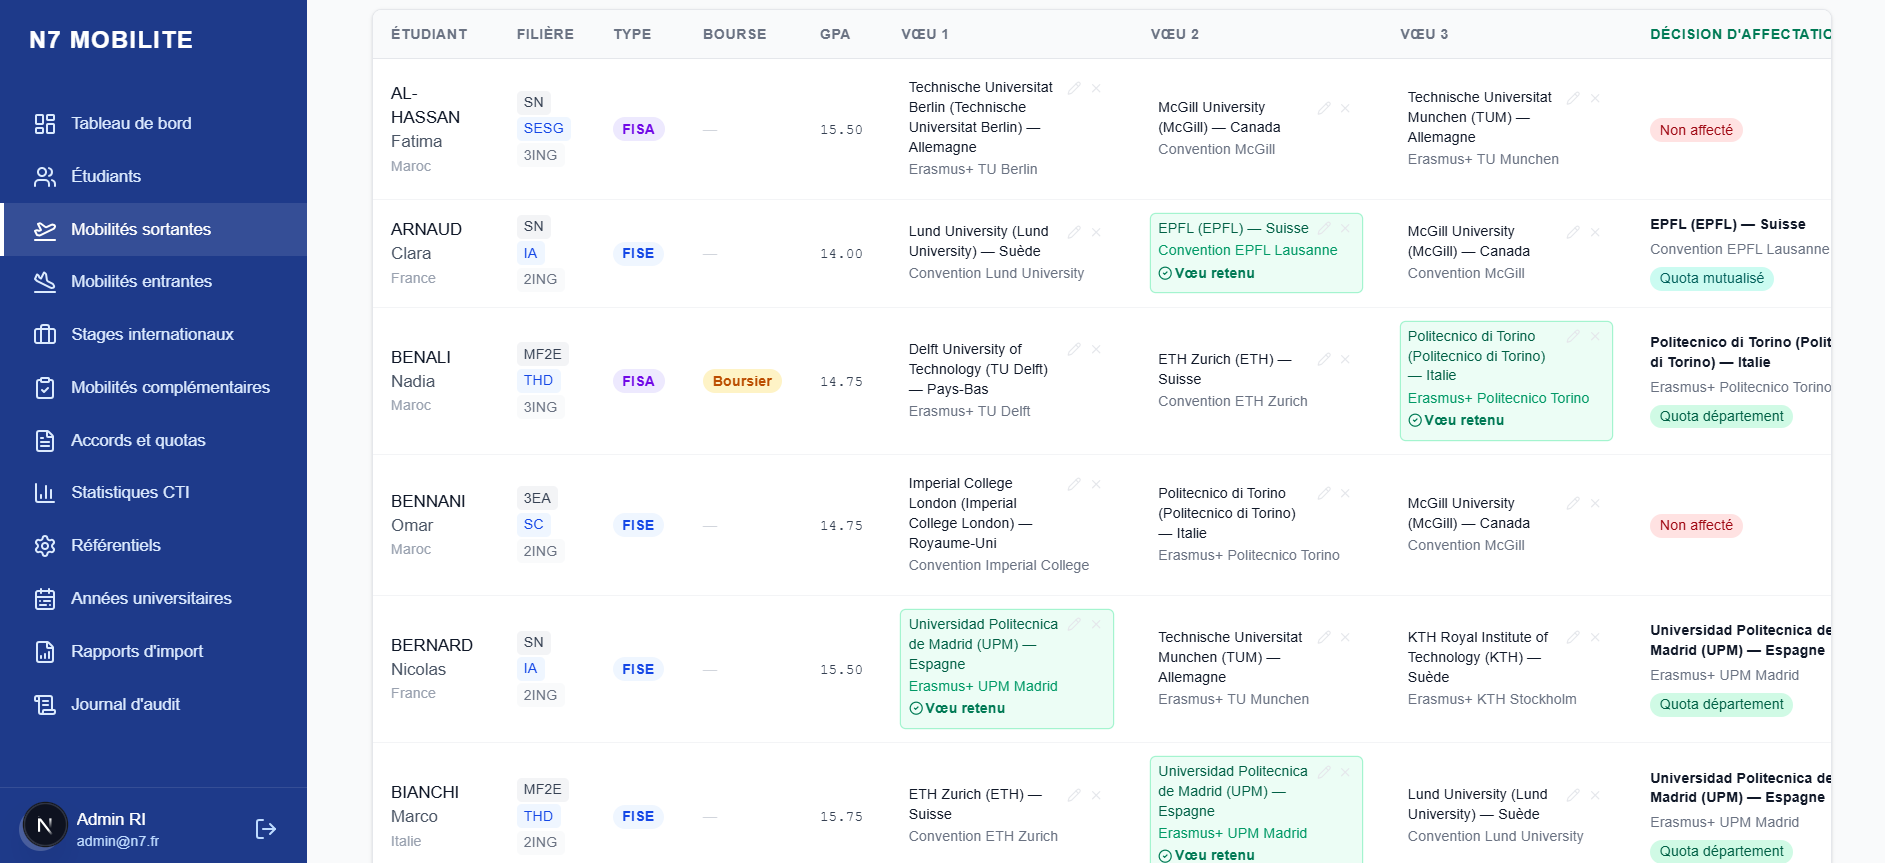
\includegraphics[width=\linewidth]{figures/captures/sprint3/sprint3-supervision.png}
  \caption{Supervision individuelle des propositions d'affectation}
  \label{fig:cap-sprint3-supervision}
\end{figure}

\begin{figure}[H]
  \centering
  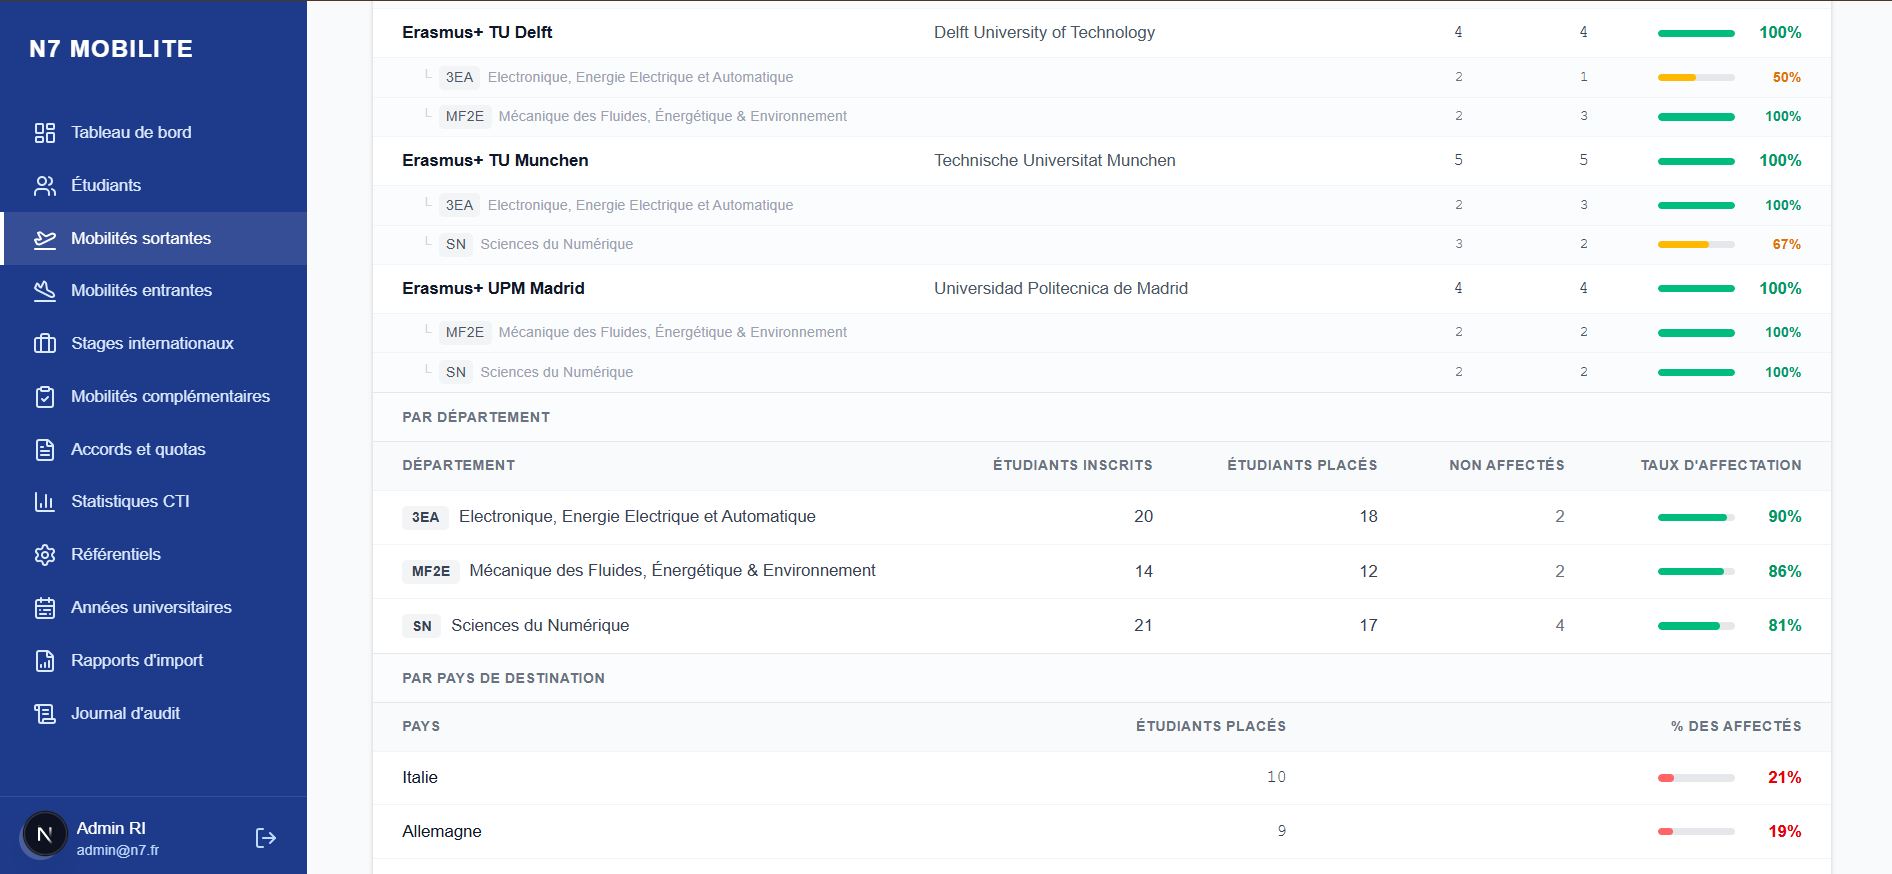
\includegraphics[width=\linewidth]{figures/captures/sprint3/sprint3-statistiques.png}
  \caption{Statistiques détaillées de l'affectation}
  \label{fig:cap-sprint3-statistiques}
\end{figure}

\bigskip
\noindent\textbf{A.2~--- Sprint 4 : consultations et mobilités complémentaires}
\par\smallskip

\begin{figure}[H]
  \centering
  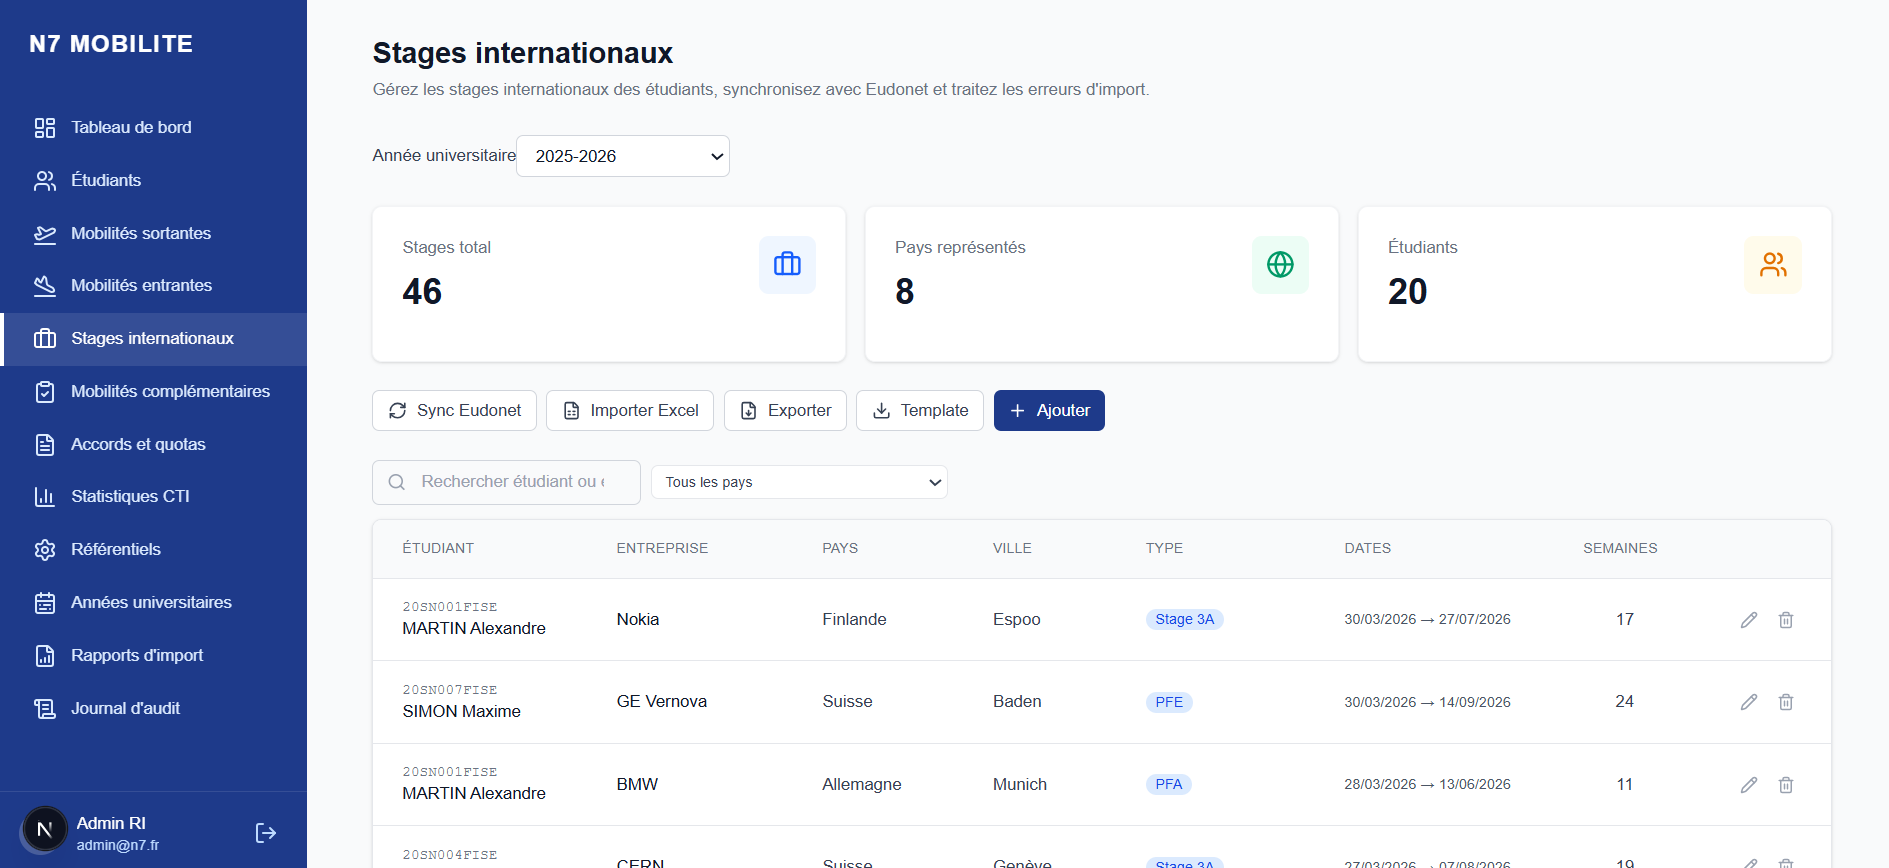
\includegraphics[width=0.85\linewidth]{figures/captures/sprint4/sprint4-stages.png}
  \caption{Consultation des stages internationaux}
  \label{fig:cap-sprint4-stages}
\end{figure}

\begin{figure}[H]
  \centering
  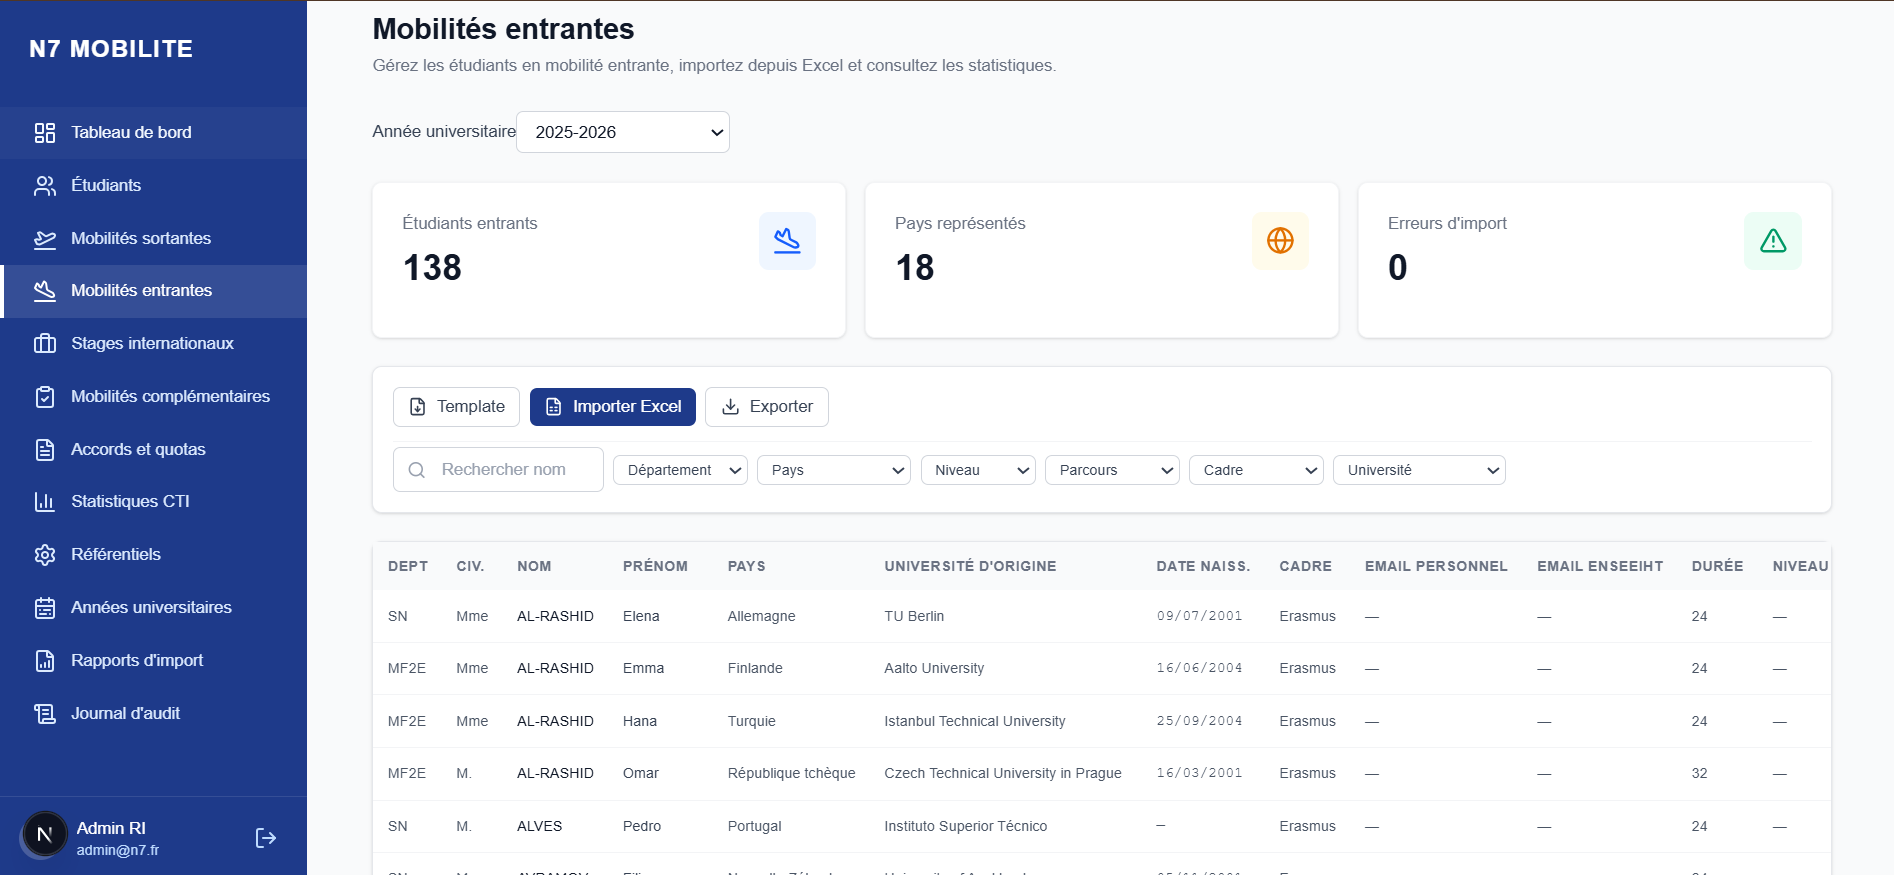
\includegraphics[width=0.85\linewidth]{figures/captures/sprint4/sprint4-entrantes.png}
  \caption{Consultation des mobilités entrantes}
  \label{fig:cap-sprint4-entrantes}
\end{figure}

\begin{figure}[H]
  \centering
  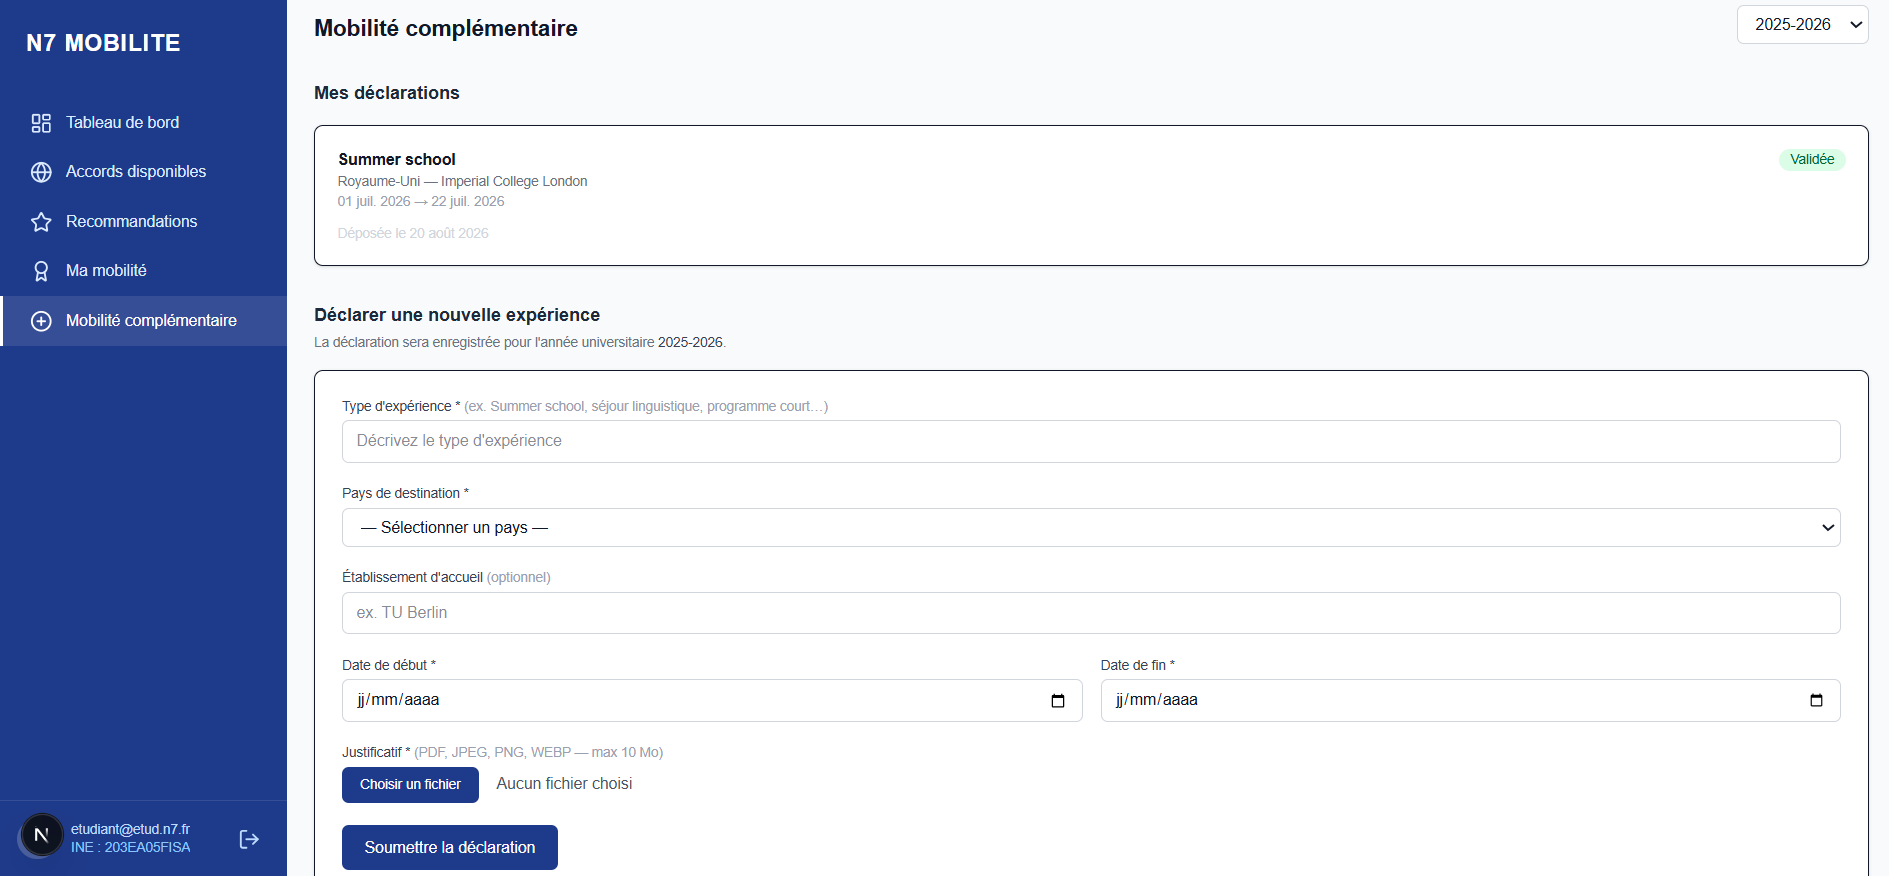
\includegraphics[width=0.85\linewidth]{figures/captures/sprint4/sprint4-declaration-etudiant.png}
  \caption{Déclaration d'une mobilité complémentaire (espace étudiant)}
  \label{fig:cap-sprint4-declaration}
\end{figure}

\begin{figure}[H]
  \centering
  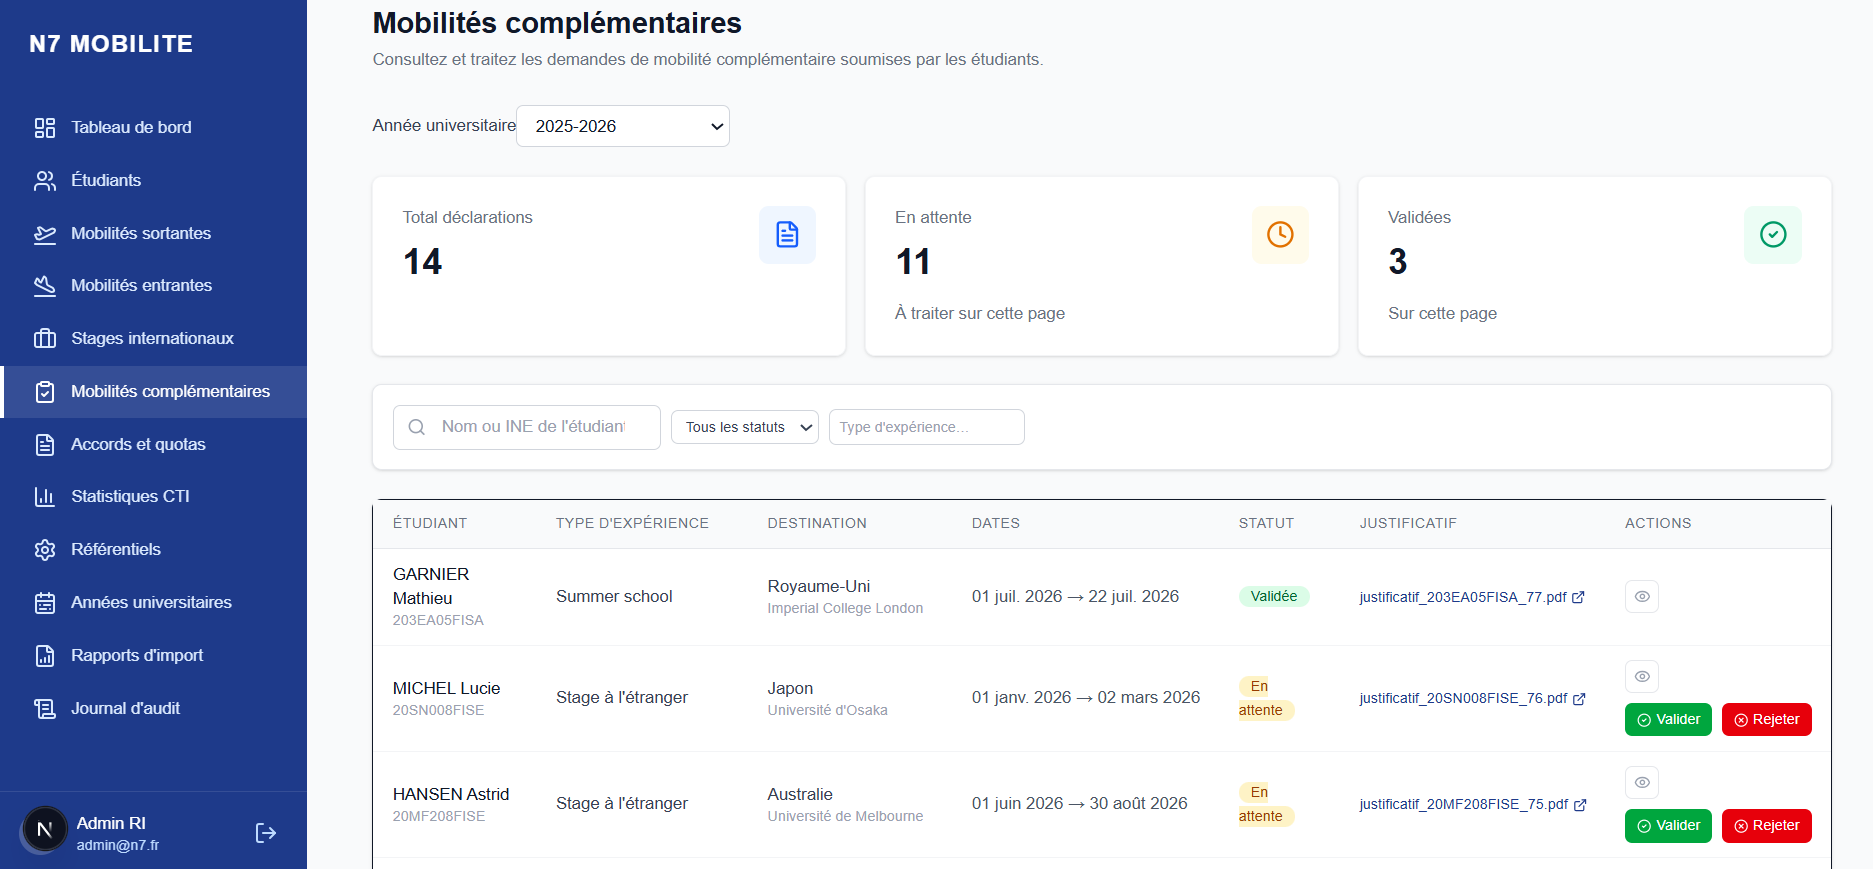
\includegraphics[width=0.85\linewidth]{figures/captures/sprint4/sprint4-mobilite-complementaire.png}
  \caption{Validation d'une mobilité complémentaire}
  \label{fig:cap-sprint4-mobilite-complementaire}
\end{figure}

\bigskip
\noindent\textbf{A.3~--- Sprint 5 : déclinaisons du tableau de bord analytique}
\par\smallskip

\begin{figure}[H]
  \centering
  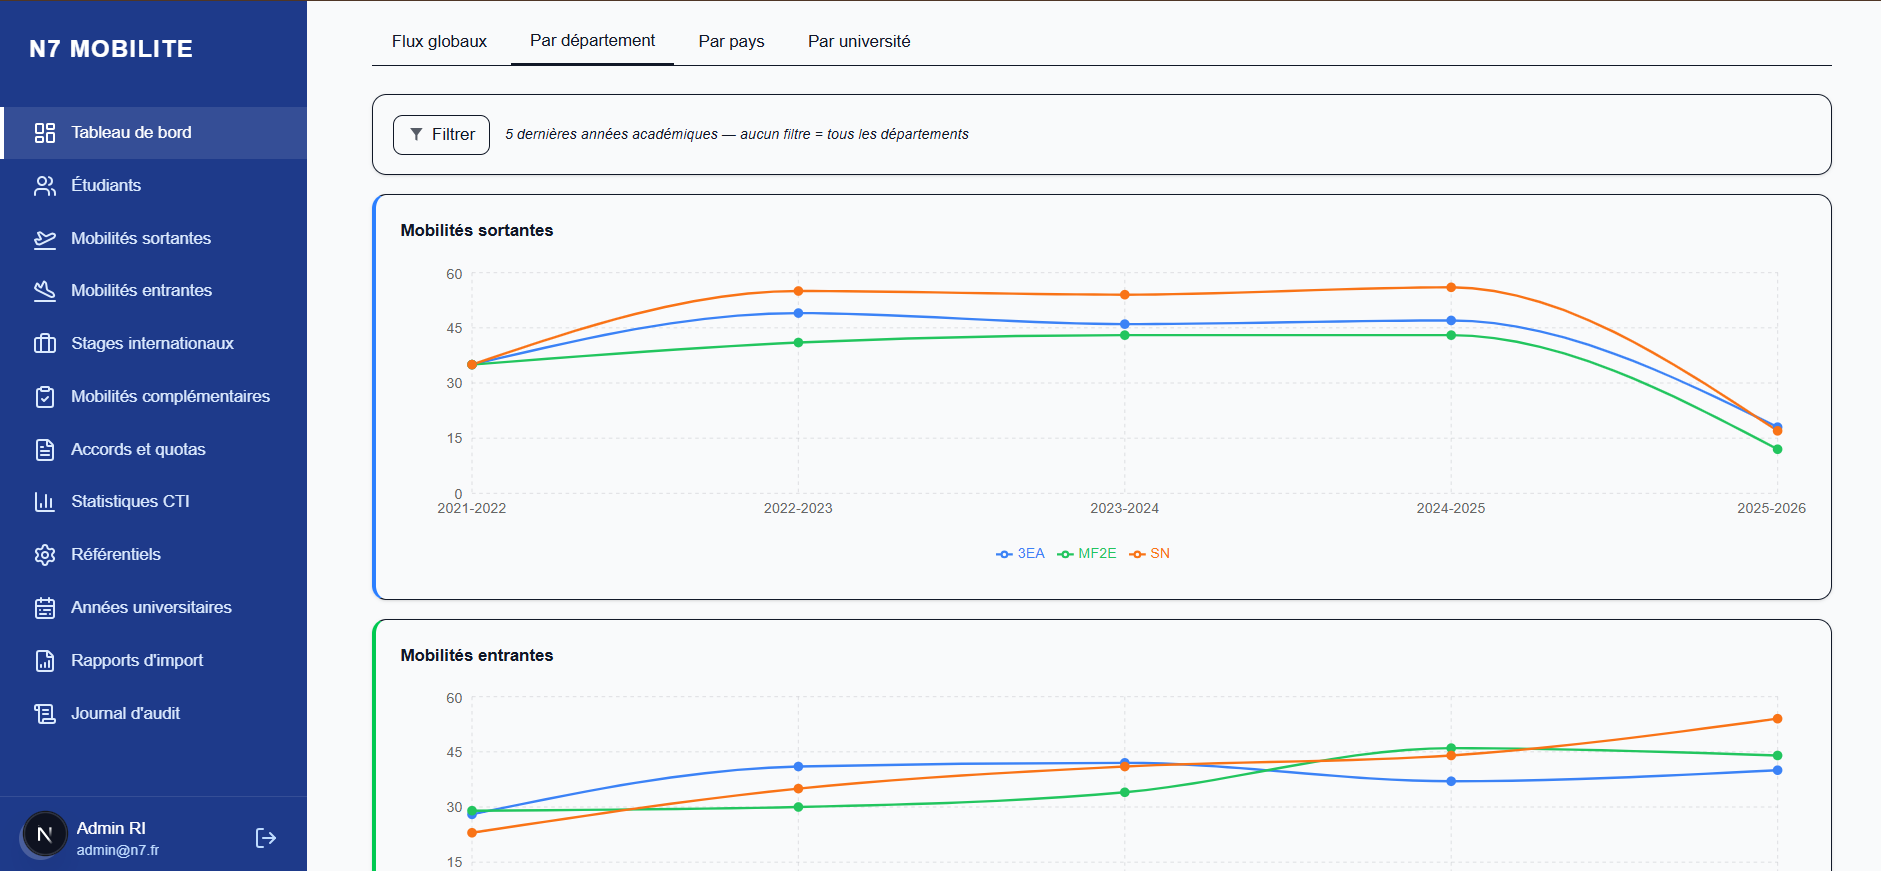
\includegraphics[width=0.85\linewidth]{figures/captures/sprint5/sprint5-dashboard-departement.png}
  \caption{Tableau de bord analytique : répartition par département}
  \label{fig:cap-sprint5-departement}
\end{figure}

\begin{figure}[H]
  \centering
  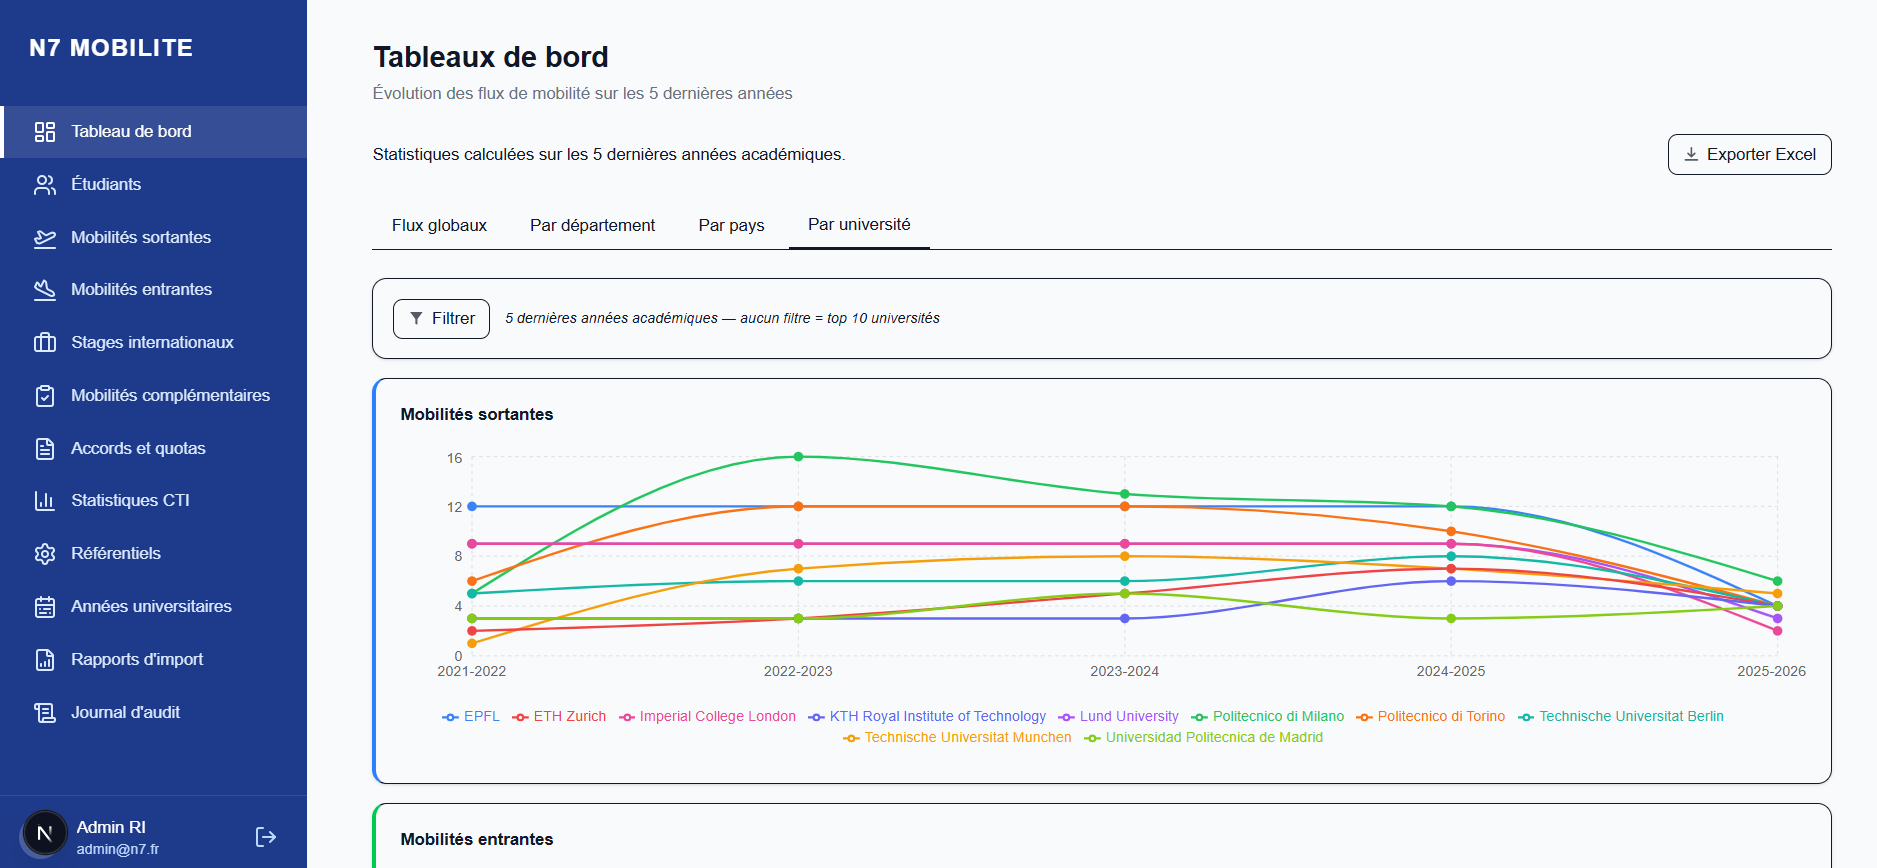
\includegraphics[width=0.85\linewidth]{figures/captures/sprint5/sprint5-dashboard-universite.png}
  \caption{Tableau de bord analytique : répartition par université partenaire}
  \label{fig:cap-sprint5-universite}
\end{figure}

\begin{figure}[H]
  \centering
  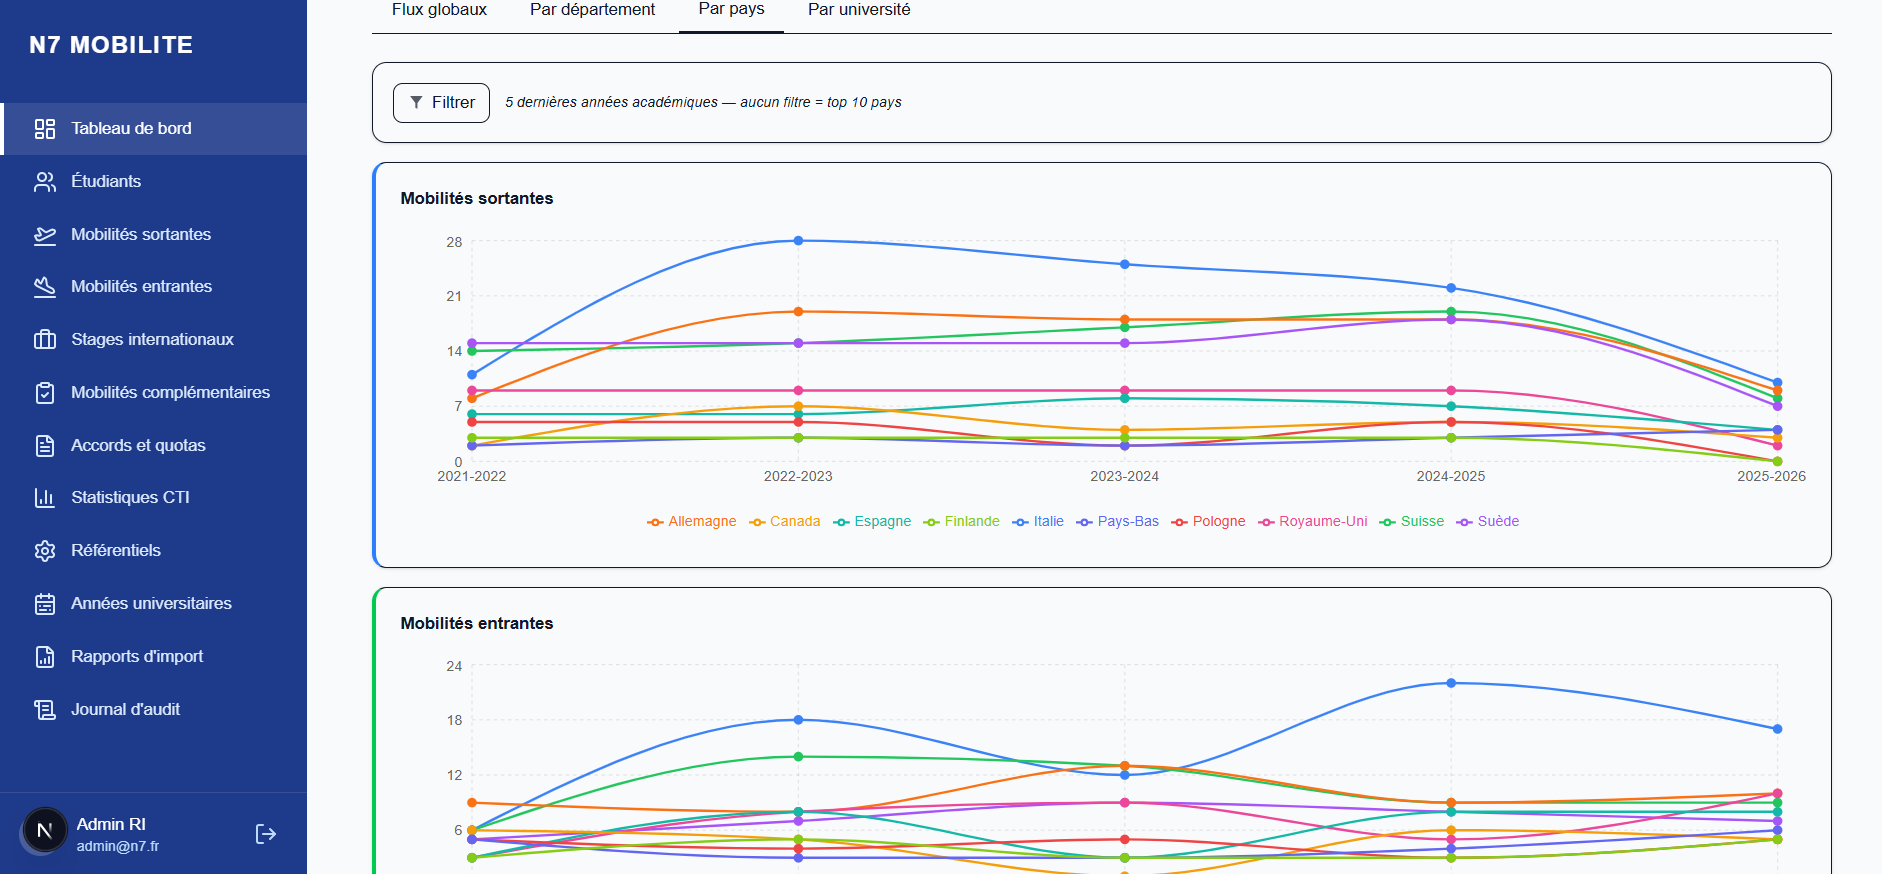
\includegraphics[width=0.85\linewidth]{figures/captures/sprint5/sprint5-dashboard-pays.png}
  \caption{Tableau de bord analytique : répartition par pays}
  \label{fig:cap-sprint5-pays}
\end{figure}

    \clearpage

 \printbibliography[heading=bibintoc,category=scientifique,title={Bibliographie}]
 \printbibliography[heading=bibintoc,notcategory=scientifique,title={Netographie}]
   
\end{document}

